This section contains experimental results from the experiment conducted to find the best possible price predicting solution. The results are divided into 4 experiments. The first experiment finds the best combination of input parameters for the network. These input parameters count meteorological, social and seasonal factors - which we identified in the analysis section~\ref{sec:Price}. The next experiment identifies the need for trimming and reasons to why it is needed in this particular dataset. The third experiment tests how different calculated inputs can include the immediate historical curve behavior in the dataset. This includes scatter, slope calculation, skewness analysis and historical EWMA(Exponentially-Weighted Moving Average). The fourth experiment takes care of the Artificial Neural Network parameters. This includes black-box optimization of epochs and the size of the dataset.

\subsection{Experiment one: Inputs}
\label{sec:priceExperimentOne}
This section is based on the input parameters that we identified in section~\ref{sec:Price}. We did a cross comparison of all the inputs and possible combinations. The last known price and the predicted demand are basic measures when you define a price in any markets and that is why we include them in every prediction. We did not make a cross comparison of the Month of Year and the Seasons of Year since they denote the same but with different granularity. We did a cross comparison both with and without matrix inputs and with a mix of non-matrix and matrix inputs. This is done to determine whether an input makes better sense on matrix form or just as a simple normalized value. 

\subsubsection{Variables}
Experiment one is based on a dataset consisting of the last 3 months averaging to 2189 hours. We use 200 epochs for each training iteration.

The parameters being examined in this test are the following:
\begin{enumerate}
	\item Last Hours Price (P)
	\item The Demand (D)
	\item Wind Speed(WS)
	\item Temperature(T)
	\item The Hourly Time of Day (ToD)
	\item The Day of the Week(DoW)
	\item The Month of the Year(MoY)
	\item The Season of the Year(SoY)
\end{enumerate}

The (M) is for Matrix input and states if the input in the time-related rows(ToD, WoD, MoY, SoY) are represented as a matrix.

The table~\ref{table:Top20Prices} contains the following information as well:
\begin{enumerate}
	\item Number in table (\#)
	\item First hidden layer neuron count (H1)
	\item Second hidden layer neuron count (H2)
	\item \% ranking from first entry (Dev)
	\item Mean Average Error (MAE)
	\item The Day of the Week(DoW)
	\item The Month of the Year(MoY)
	\item The Season of the Year(SoY)
\end{enumerate}

\subsubsection{Hypothesis}
This is the first and most comprehensive of the tests conducted for price prediction. In this experiment we want to test all the different combinations of the parameters. We expect to see a better curve-fit as we include more variables and more complex variables. In regard to the dataset analysis in section~\ref{sec:ElectricityPriceAnalysis} we see the connection between the aforementioned variables and the price (that we are trying to predict). We have the following expectations based on the dataset analysis:
\begin{enumerate}
	\item The Wind Speed will show a positive impact on the price because of the correlation between the two. Also the wind speed impacts the production of green energy which impacts the overall price of energy. Since the wind power production accounts for about 25\%(see data analysis in section ~\ref{sec:Price}) of the complete power production in western Denmark we also expect to see that this parameter will increase accuracy.
	\item The Temperature might have a small impact on the price but there is nearly no correlation between the price and the temperature. If it should have an impact it is probably because of the correlation between the temperature and the demand thus indirect influencing the price.
	\item The Hourly Time of Day is going to have an effect on the hourly predicted price. The reason being the correlation between the price and what time of day it is and because we are predicting the hourly price; which logically indicates that this parameter is important for such a prediction. 
	\item The Day of the Week, The Month of the Year and The Seasons of the Year is expected to have a positive impact on the prediction. The impact are expected to get smaller as the inputs become more general e.g season of year; since our training dataset is based on 1/4 of a year. 
	\item Matrix representation will be better than single node representation of the seasonality. This is due to the fact that matrix is a more granulated input format than single node. This has also been discussed in section~\ref{sec:Matrix}.
\end{enumerate}

\subsubsection{Results}
We present the results from this experiment in table~\ref{table:Top20Prices}. The input parameters will be analyzed one by one in the next subsections. After that we will talk about some of the problems with some of these input parameters.

\begin{table}[H]
\centering  % used for centering table
\resizebox{\textwidth}{!}{
\begin{tabular}{|c|c|c|c|c|c|c|c|c|c|c|c|c|} % centered columns (7 columns)
\hline
{\#} & P & D & WS & T & ToD & DoW & MoY & SoY & H1 & H2 & MAE & {\%} ranking\\ [0.5ex] % inserts table 
%heading
\hline                  % inserts single horizontal line
1  &  \x    & \x    & \x    & \x    & \x\m  & \x\m  &       & \x\m  & 7  & 8  & 57.12 &  - \\ \hline
2  &  \x    & \x    & \x    & \x    & \x\m  & \x    &       & \x\m  & 5  & 9  & 58.09 & 1.7\% \\ \hline
3  &  \x    & \x    & \x    & \x    & \x\m  &       & \x\m  &       & 6  & 11 & 58.79 & 2.92\% \\ \hline
4  &  \x    & \x    & \x    &       & \x\m  & \x\m  & \x\m  &       & 9  & 3  & 60.14 & 5.29\% \\ \hline
5  &  \x    & \x    & \x    & \x    & \x\m  & \x    &       &       & 16 & 8  & 62.19 & 8.88\% \\ \hline
6  &  \x    & \x    & \x    & \x    & \x\m  &       &       & \x\m  & 6  & 5  & 62.26 & 9.0\% \\ \hline
7  &  \x    & \x    & \x    & \x    & \x\m  & \x    & \x\m  &       & 5  & 8  & 62.84 & 10.01\% \\ \hline
8  &  \x    & \x    & \x    & \x    & \x    & \x    &       & \x\m  & 5  & 0  & 63.94 & 11.94\% \\ \hline
9  &  \x    & \x    & \x    & \x    & \x    & \x\m  & \x\m  &       & 5  & 4  & 64.19 & 12.38\% \\ \hline
10 &  \x    & \x    & \x    &       & \x\m  & \x    & \x\m  &       & 6  & 8  & 64.72 & 13.31\% \\ \hline
11 &  \x    & \x    & \x    &       & \x    & \x    & \x\m  &       & 5  & 5  & 65.07 & 13.92\% \\ \hline
12 &  \x    & \x    & \x    & \x    & \x\m  & \x\m  &       &       & 6  & 6  & 65.95 & 15.46\% \\ \hline
13 &  \x    & \x    & \x    & \x    & \x\m  & \x\m  & \x\m  &       & 7  & 12 & 66.55 & 16.51\% \\ \hline
14 &  \x    & \x    & \x    &       & \x    &       &       & \x\m  & 7  & 0  & 67.21 & 17.66\% \\ \hline
15 &  \x    & \x    & \x    & \x    & \x    & \x    &       &       & 5  & 0  & 67.88 & 18.84\% \\ \hline
16 &  \x    & \x    & \x    &       & \x    & \x    &       & \x    & 6  & 0  & 68.21 & 19.42\% \\ \hline
17 &  \x    & \x    & \x    &       & \x\m  & \x\m  &       &       & 8  & 6  & 68.34 & 19.64\% \\ \hline
18 &  \x    & \x    & \x    &       & \x\m  &       &       & \x\m  & 7  & 4  & 68.35 & 19.66\% \\ \hline
19 &  \x    & \x    & \x    & \x    & \x    & \x    & \x    &       & 6  & 0  & 68.43 & 19.8\% \\ \hline
20 &  \x    & \x    & \x    & \x    & \x    &       &       & \x\m  & 5  & 0  & 68.45 & 19.84\% \\ \hline
\end{tabular}
}
\caption{The top 20 results on training set 3 last months} % title of Table
\label{table:Top20Prices} % is used to refer this table in the text
\end{table}

\subsubsection{Wind speed}
If we take a look at the top 20 best input combinations (shown in table~\ref{table:Top20Prices}) we see some clear trends. We will start analyzing the data from left to right. The price and demand are static as mentioned earlier since they are fundamental market forces and thus not a changing factor in this analysis. The next input parameter is the Wind Speed. We see that every input combination in the top 20 includes the wind production and it is therefore a must for the prediction of the energy prices. The 72 first inputs(the 50\% best results) contains only two combinations that does not have wind speed in them. Also we saw in section~\ref{sec:windPowerAnalysis}(table~\ref{table:pearsonCoeficientWindProduction}) that the Wind Speed heavily influences the green energy production and thus influencing the energy prices. If we remove wind speed from the \#1 combination it ends up at place \#70 which are 37.55\% worse than the best result. In graph~\ref{fig:Windspeed_no_windspeed} we see that the prediction without wind speed has a tendency to overshoot more than the one with wind speed does which over a whole year sums up to a significant difference. \todo{Vis hele grafen i bilaget?}

\begin{figure}[H]
\centering
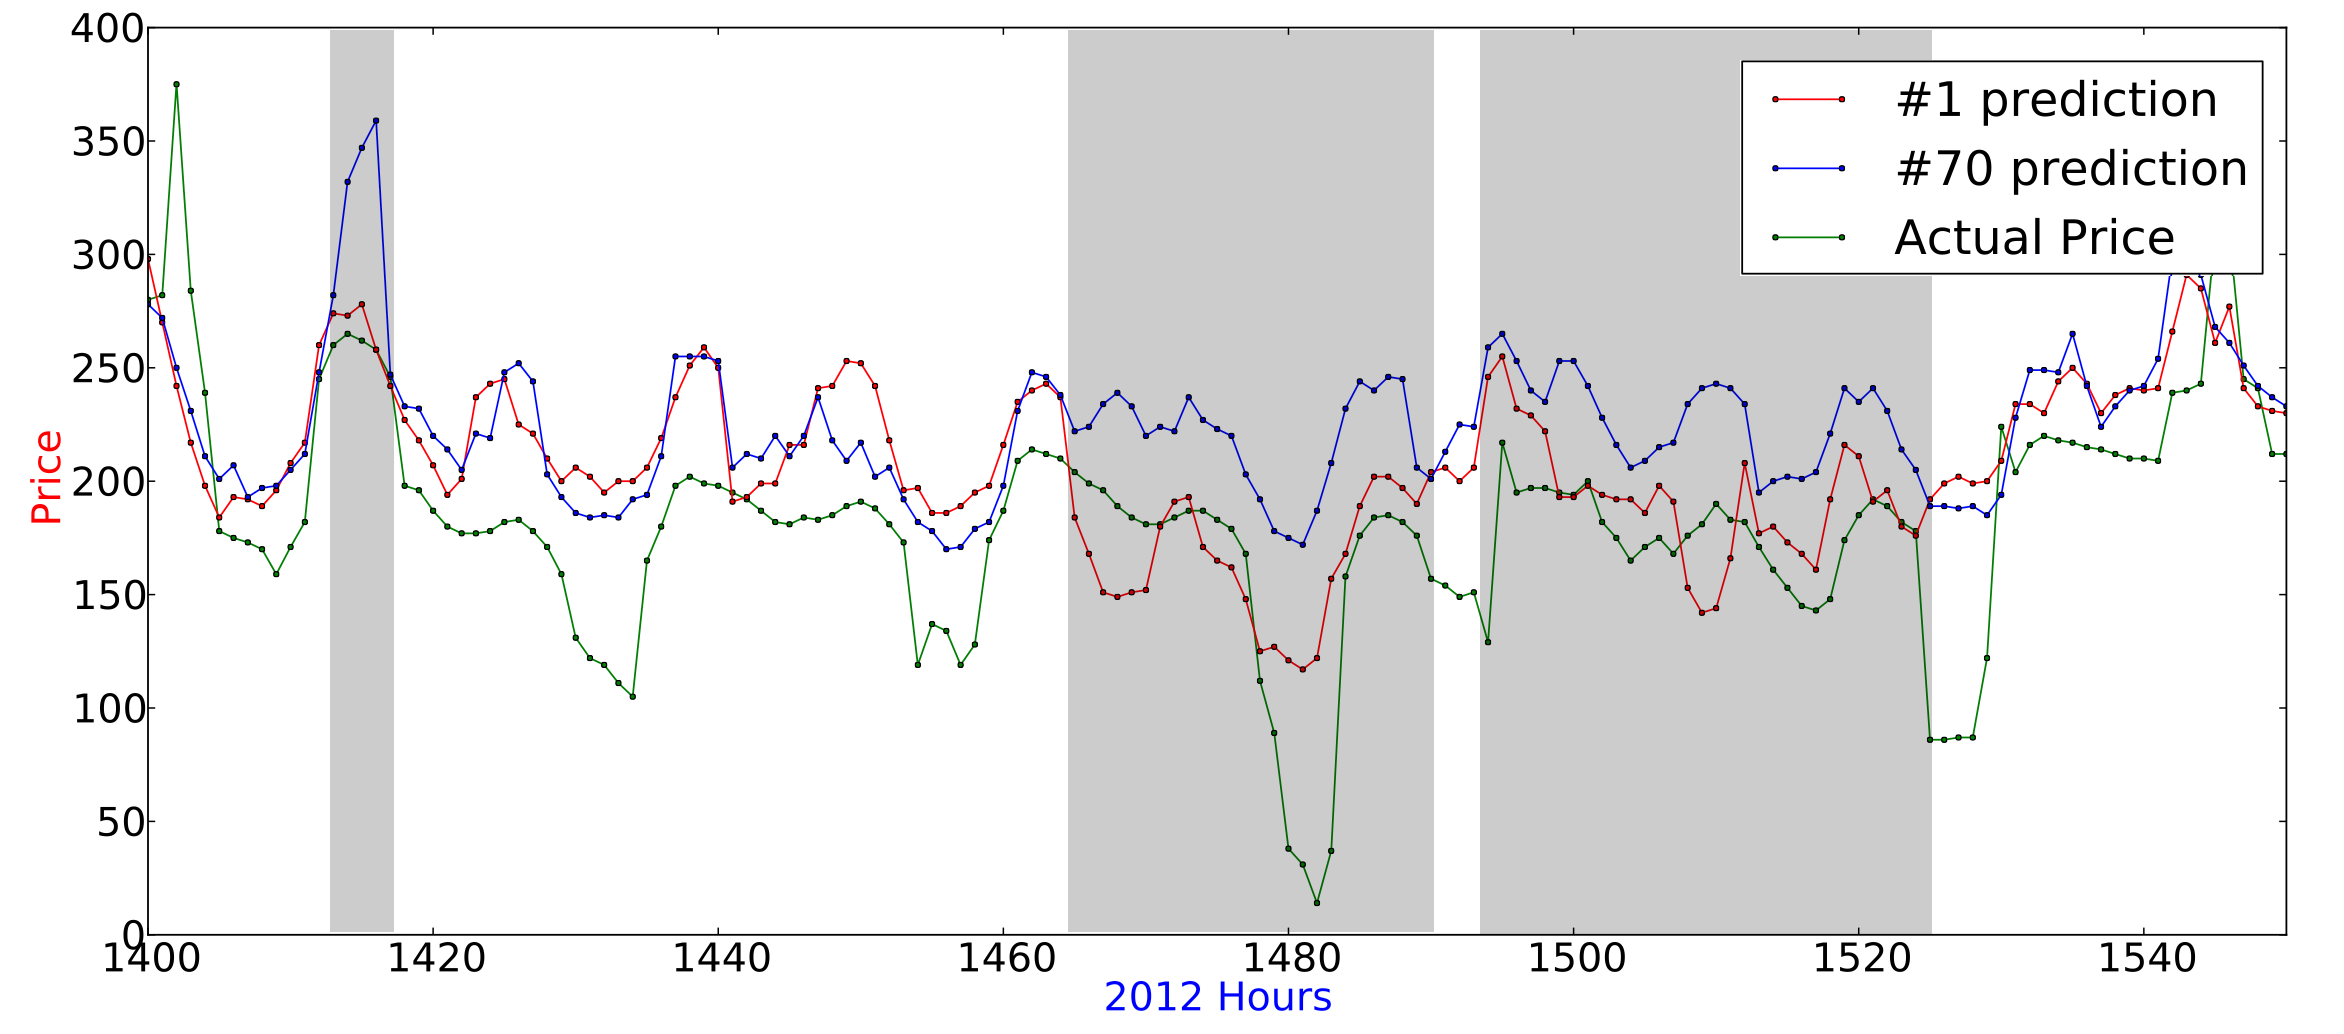
\includegraphics[width=\linewidth]{billeder/PriceExperimentalAnalysis/X1_windspeed_vs_no_windspeed.png}
\caption{\#1 forecast from table~\ref{table:Top20Prices} with and without wind speed}
\label{fig:Windspeed_no_windspeed}
\end{figure}

\subsubsection{Temperature}
The temperature is a less obvious candidate for the prediction of price since the Pearson's correlation between the two only are 0.17. Nevertheless it is showing up in 8/10 top combinations in table~\ref{table:Top20Prices} and this might be because of the correlation between temperature/demand which is -0.59. The temperature is scattered all over the 144 combinations and thus it is hard to say something concrete about this input variable. The best result without temperature is at place 4 in table~\ref{table:Top20Prices} and the same one with temperature is at place 13 with a difference between the two of 10.66\%. Graph~\ref{fig:temperature_comparison} shows that there is no significant difference between the two combinations. In both of them the ANN is overshooting the targetat different spots.

\begin{figure}[H]
\centering
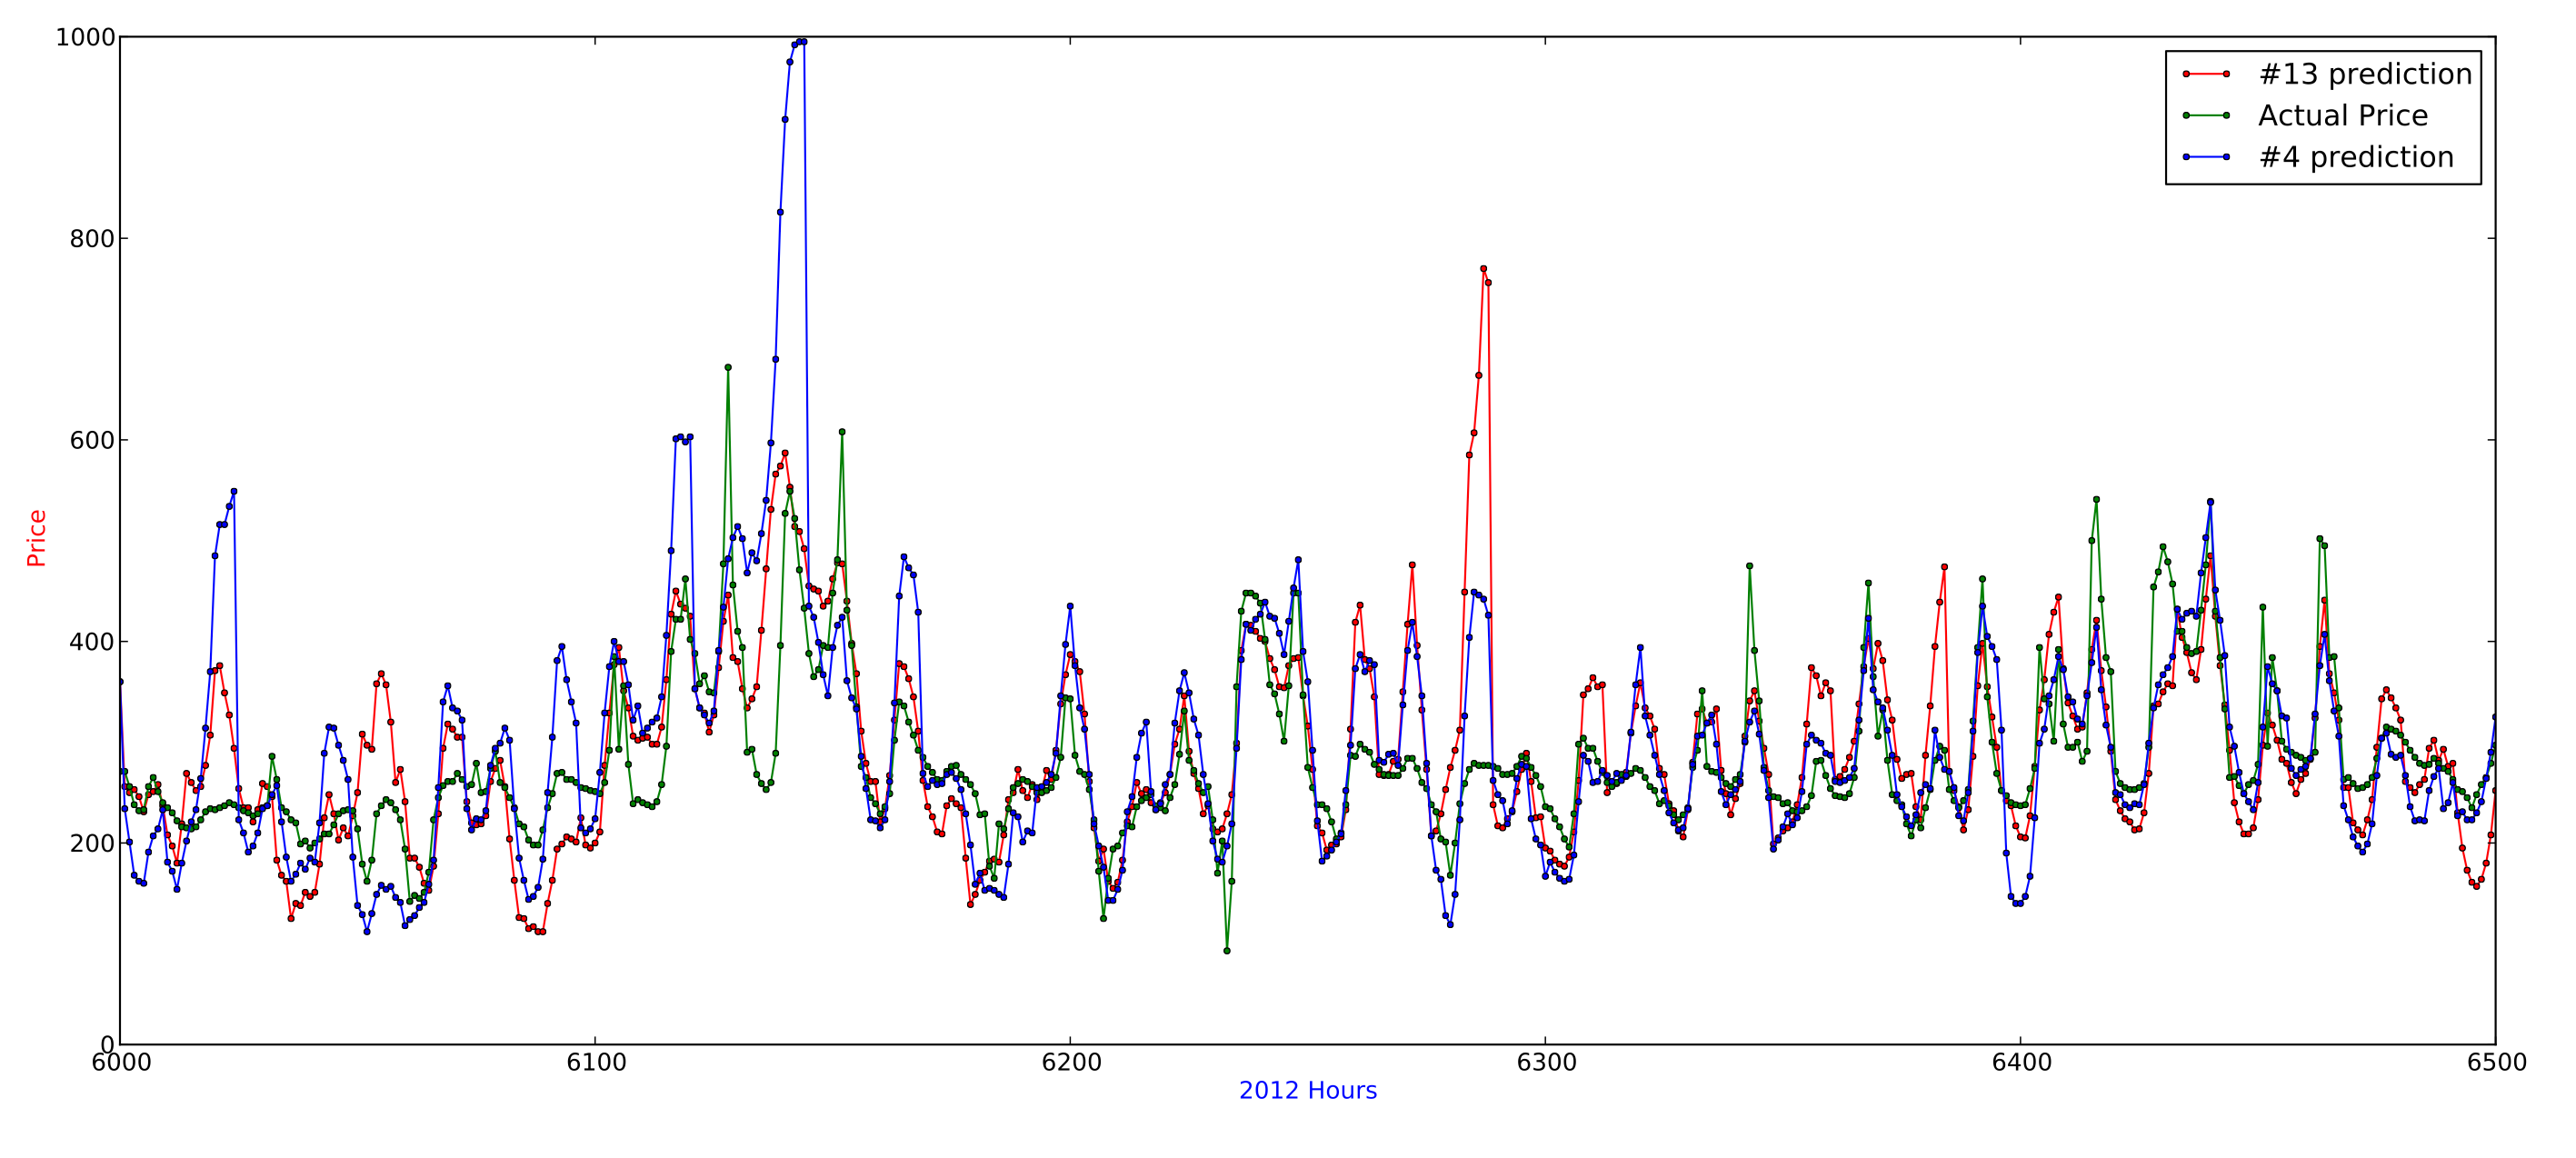
\includegraphics[width=\linewidth]{billeder/PriceExperimentalAnalysis/temperatureComparison.png}
\caption{\#4 forecast from table~\ref{table:Top20Prices} with and without temperature}
\label{fig:temperature_comparison}
\end{figure}

\subsubsection{The Hourly Time of the Day}
The Hourly Time of Day (ToD) is included in every single combination in the top 20. This clearly shows that this input parameter is important for the prediction of the price. This is kind of obvious since what we are predicting is the hourly price. In section~\ref{sec:seasonality}(figure~\ref{fig:price_per_hour}) we saw that the price varied from 190 to 335 which strengthens the importance of the relationship between time of day and the price. Also the top 7 all have the ToD on matrix form which indicates that this is the best way of representing the ToD. The comparison between \#1 prediction with Time of Day and the one without \#55 we see a difference of 31.85\% and we did a graph comparison of the two shown in figure~\ref{fig:dowComparison}. Here we see that the one with ToD (\#1) are better at following the curve compared to the prediction without Time of Day. The prediction without Time of Day seems to follow an average between the high and low spikes instead of following the curve up and down. This makes sense since the ToD interprets into what hours have high prices and which that have low prices.

\begin{figure}[H]
\centering
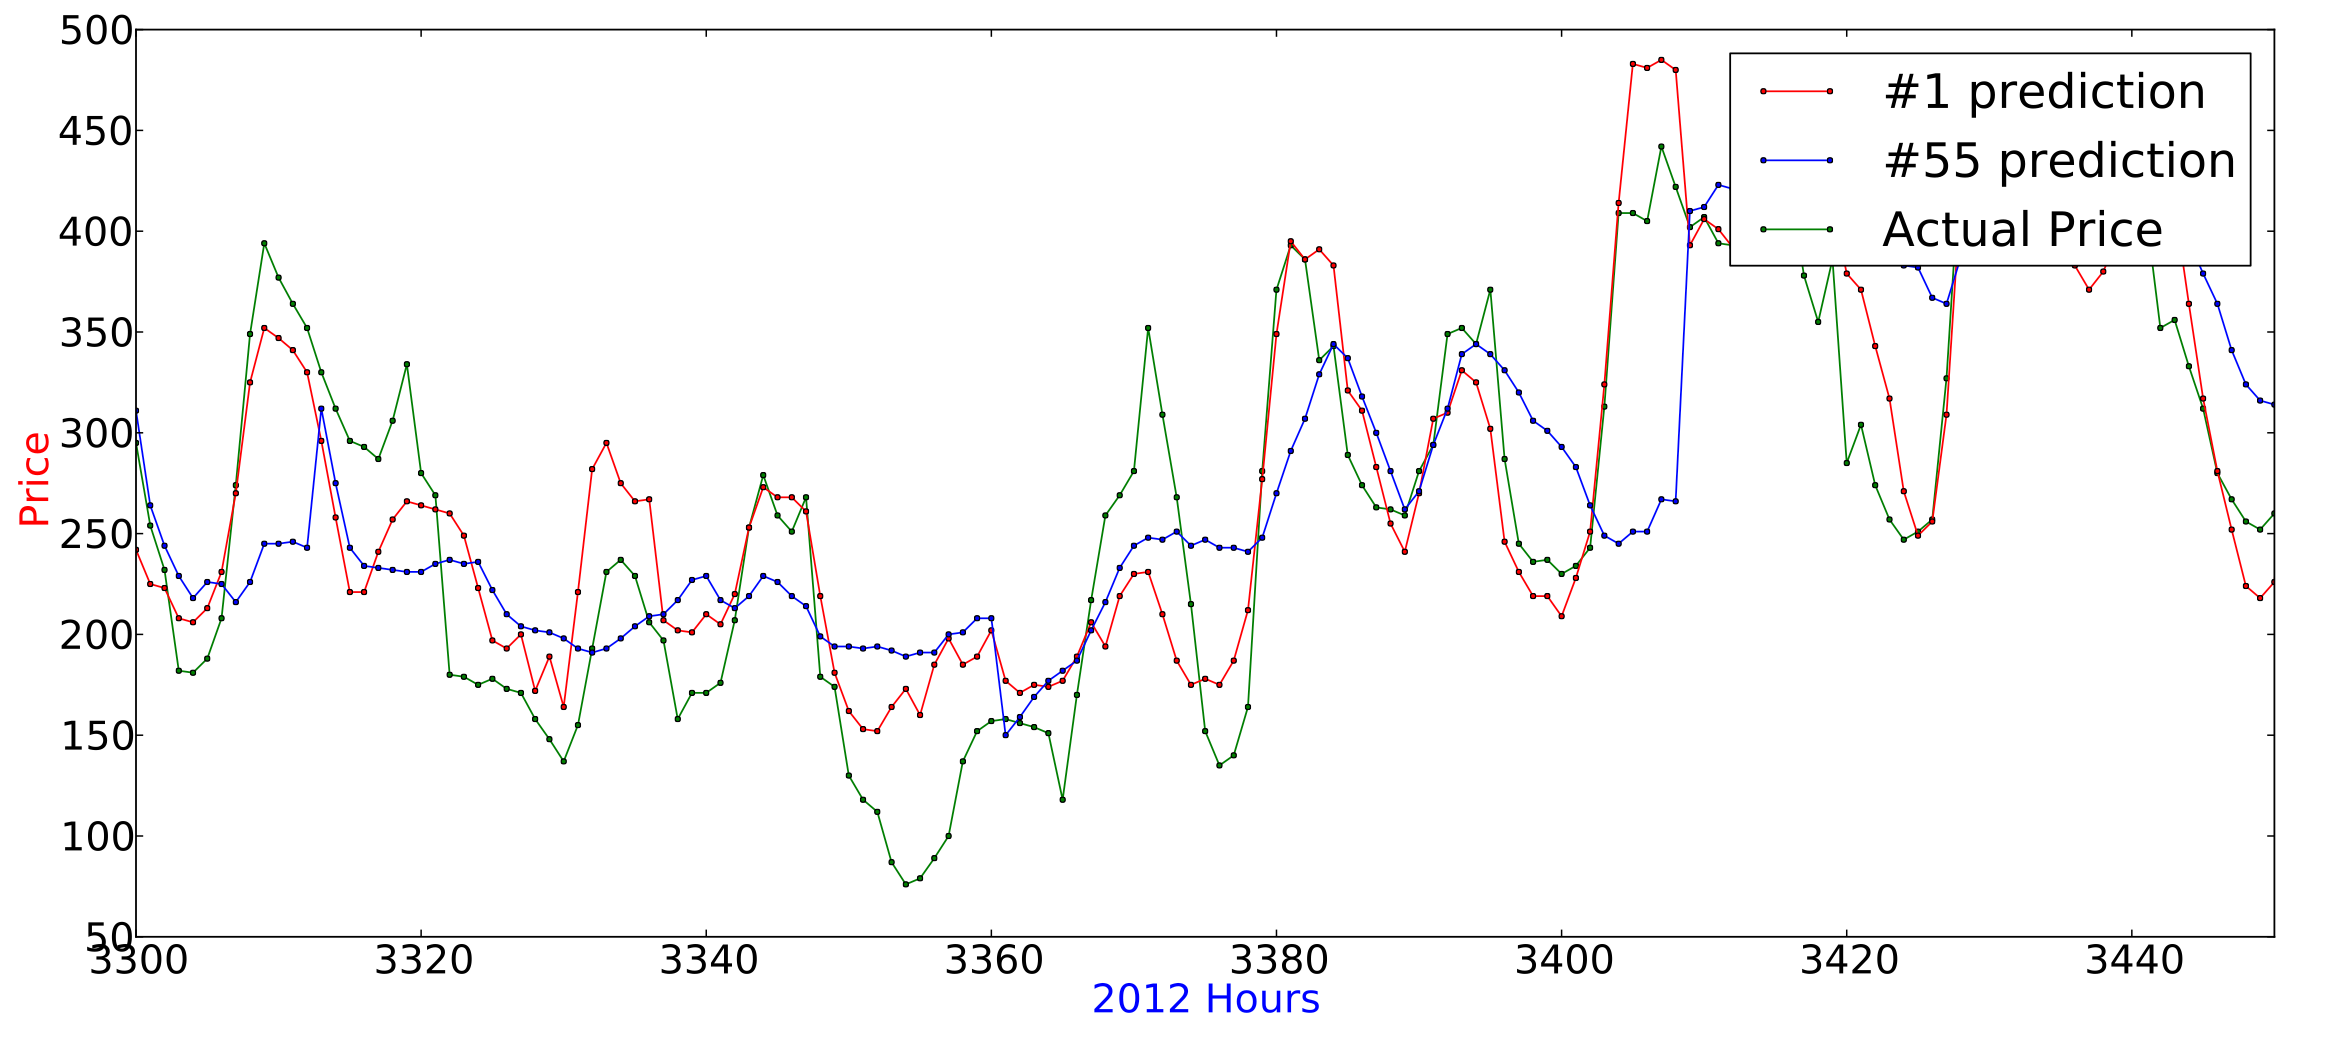
\includegraphics[width=\linewidth]{billeder/PriceExperimentalAnalysis/dowComparison.png}
\caption{\#1 forecast from table~\ref{table:Top20Prices} with and without Time of Day}
\label{fig:dowComparison}
\end{figure}

\subsubsection{The Day of the Week}
Next we have the Day of the Week (DoW) parameter. This parameter are present in 75\% of the 20 best results (8/10 and in 15/20 best combinations). We have to believe that it plays a significant role in the prediction of price. If we look at the analysis of the average price over weekdays in section~\ref{sec:seasonality}(figure~\ref{fig:price_over_weekdays}) we see that there is a significant difference in price on the different days. This is especially present in the weekdays compared to the weekend. This parameter is mixed between matrix input and standard input. This might be due to the fact that the biggest difference between days are weekend and weekday thus minimizing the effect of a matrix representation. \todo{Maaske lav et forsoeg med weekday/weekend matrix.}

\subsubsection{The Season of Year features}
The last two parameters - Month of Year(MoY) and Season of Year (SoY) - are codependent and will be covered together. As mentioned before they cover the same information and we therefore only need one of them at any time \todo{Lav forsoeg der viser at det ikke giver mening at have baade MoY og SoY paa samme tid.}. The values are present in 9/10 of the best combinations in ~\ref{table:Top20Prices}. This is an indicator that the seasonality in the form of MoY and SoY plays a role in predicting the electricity price. Also we saw in the analysis in section~\ref{sec:seasonality}(figure~\ref{fig:monthlyAveragePrice} and ~\ref{fig:seasons}) that the price changes with seasonality and that it especially was more expensive in the winther than the rest of the year.

\subsubsection{Matrix}
The matrix representation in the top 20 is the most common representation of the seasonal inputs (ToD, DoW, MoY and SoY) - with only 3/20 containing no matrix at all. The matrix format was expected to give a better result based on what we discussed in the matrix section~\ref{sec:Matrix}. The 3 combinations that does not contain a matrix representation are already present in the top 20 as pure matrix form. This might be the combination of inputs variables that are a good since both the matrix form and the non-matrix form are represented in the top 20 best combinations.

In the Wind Production Experiments section~\ref{sec:windProductionExperiments} we conducted a separate experiment for the matrix analysis. We did a combined experiment in this section because we had 4 different parameters that can be represented as a matrix thus giving us a lot of different combinations. We also wanted to test all of the different combinations of matrix and non-matrix inputs because a mixed combination might render a better solution e.g. the season of year shifts so rarely it might be a better representation (together with the other parameters) on non-matrix form. Also there might be combinations with the rest of the inputs that work better with the matrix-format than others.

\todo{Referer til Brians. Han har allrede skrevet om Matrix i forhold til at hans ikke virker specielt overbevisende, men at det i mit virker meget bedre. Diskuter.}

\begin{table}[H]
\centering  % used for centering table
\resizebox{\textwidth}{!}{
\begin{tabular}{|c|c|c|c|c|c|c|c|c|c|c|} % centered columns (7 columns)
\hline
P & D & WS & T & ToD & DoW & MoY & SoY & MAE & \% ranking\\ [0.5ex] % inserts table 
%heading
\hline                  % inserts single horizontal line
 \x    & \x    & \x    &       &       & \x\m  & \x\m  &       & 105.70 & \#134 \\ \hline
 \x    & \x    &       &       &       & \x\m  &       & \x\m  & 107.85 & \#135 \\ \hline
 \x    & \x    &       & \x    & \x    &       & \x    &       & 108.37 & \#136 \\ \hline
 \x    & \x    &       & \x    &       &       & \x    &       & 111.14 & \#137 \\ \hline
 \x    & \x    &       & \x    &       &       & \x\m  &       & 111.65 & \#138 \\ \hline
 \x    & \x    &       & \x    &       & \x\m  & \x\m  &       & 113.56 & \#139 \\ \hline
 \x    & \x    &       & \x    &       &       &       & \x    & 115.29 & \#140 \\ \hline
 \x    & \x    &       &       &       &       & \x\m  &       & 115.81 & \#141 \\ \hline
 \x    & \x    &       & \x    &       & \x\m  &       & \x\m  & 115.83 & \#142 \\ \hline
 \x    & \x    &       & \x    &       & \x    & \x    &       & 117.17 & \#143 \\ \hline
 \x    & \x    &       &       &       & \x\m  & \x\m  &       & 117.34 & \#144 \\ \hline
\end{tabular}
}
\caption{The bottom 10 input combinations for price prediction} % title of Table
\label{table:Bottom10Prices} % is used to refer this table in the text
\end{table}

If we take a look at the bottom 10 input combinations in terms of MAE we see some tendencies as well. We see that Wind Speed only appears in one of the combinations and so does the Time of Day(And not in the same combination). This further strengthens that these two variables are very important for the price prediction. We talked about matrix form earlier and its impact on the combinations. In the bottom 20 table we see that there is a lot of the combinations that contains variables on matrix form. This is because the Wind Speed and the Time of Day are the most influential parameters thus sending the combinations with these absent to the bottom of the chart. As these combinations also include matrix forms they will occur in the bottom top 20 thus not indicating that matrix form has no effect on the dataset.

\begin{table}[H]
\centering  % used for centering table
\resizebox{0.4\textwidth}{!}{
\begin{tabular}{|c|c|c|} % centered columns (7 columns)
	\hline
	{\#} & 3 Months & 4 Months \\ [0.5ex] % inserts table 
	%heading
	\hline  
	 1  & 57.12 & 61.70  \\ \hline
	 2  & 58.09 & 68.23  \\ \hline
	 3  & 58.79 & 63.80  \\ \hline
	 4  & 60.14 & 67.82  \\ \hline
	 5  & 62.19 & 74.89  \\ \hline
	 6  & 62.26 & 61.86  \\ \hline
	 7  & 62.84 & 62.62  \\ \hline
	 8  & 63.94 & 72.37  \\ \hline
	 9  & 64.19 & 84.12  \\ \hline
	 10 & 64.72 & 72.29  \\ \hline

	 11 & 65.07 & 79.71  \\ \hline
	 12 & 65.95 & 58.19  \\ \hline
	 13 & 66.55 & 67.31  \\ \hline
	 14 & 67.21 & 74.67  \\ \hline
	 15 & 67.88 & 77.29  \\ \hline
	 16 & 68.21 & 72.45  \\ \hline
	 17 & 68.34 & 72.31  \\ \hline
	 18 & 68.35 & 76.25  \\ \hline
	 19 & 68.43 & 75.10  \\ \hline
	 20 & 68.45 & 75.97  \\ \hline 
\end{tabular}
}
\caption{Top20(3 months) compared to 4 months run.} % title of Table
\label{table:top20comparedTo4months} % is used to refer this table in the text
\end{table}

As we saw in the wind production experiments(WPE) section~\ref{sec:windPowerAnalysis} there was a problem regarding the way we conducted tests for the seasonality; specifically for the MoY and the SoY. We only use the last 3 months to train the network and that sort of eliminates the obvious purpose of the MoY and SoY. As we saw in the results for the first experiment in WPE if we include the same month as we are in from last year and reintroduce the purpose of the SoY and MoY it gave us a worse result than leaving it out. To make sure the same thing applies on the price prediction experiments we conducted to runs of all the combinations of inputs. First we ran it with the last 3 months including the same month that we are in from last year and after that we ran the experiment with only the last 3 months.
\todo{Er det blevet skrevet?}

Table~\ref{table:top20comparedTo4months} shows us the top 20 MAE from the experiment with a training set containing the last 3 months(3 Months). We have compared this to the experiment with a training set containing the last 3 months and the same month from last year(4 Months). As we see in table~\ref{table:top20comparedTo4months} the difference between the two datasets are not that big. This also shows in the appendix~\ref{sec:priceResultAppendix} where the distribution of the MAE over the two datasets are quite similar. From this we can conclude that the effect of using last years month in our dataset does not make a significant difference and can be left out. This raises the question if the MoY and the SoY can be left out as well, since the obvious use for it is eliminated by never having a full month or a full season in the training set - that is equal to the one we predict. Even though it might be questionable what the impact really is it seems to be enhancing the performance of the ANN since these parameters are apparent in most of the best results. This can be due to the fact that it actually works as a slope analysis tool instead of the original seasonality indicator. Now it might work to differentiate the past months/seasons from the month we are predicting thus not directly affecting it but indirectly by allowing the ANN to give the past months some weight which are not applied to the current. Also it gives us some knowledge of the current month if we are in the middle of it which can be translated into slope behavior.

First we conducted an experiment containing a training set with a full year (to test the effect of seasonality on a full year) we included the rest of the parameters equal to rank \#1 in table~\ref{table:Top20Prices} and shifted the seasonality. The results can be seen in table~\ref{table:1YearTrain} where we can see the full effect of seasonality over a year. The table clearly shows that the MoY combination is the best of the three. If we compare the results to the results from table~\ref{table:Top20Prices} it shows us that with monthly seasonality the neural network will be able to do the same predictions as the predictions that only have a training set of 3 months. With the possibility of over training in too large datasets(see paper~\cite{1}) and that the neural network takes longer time training on a larger dataset. We can conclude that the smaller dataset of 3 months are better to use than the full year (We will elaborate on this in experiment X)\todo{Saet rigtigt experiment}. Further more we have to test if seasonality being an input parameter makes sense when our dataset is only 3 months big.

\begin{table}[H]
\centering  % used for centering table
\begin{tabular}{|c|c|c|c|c|c|c|c|c|c|c|} % centered columns (7 columns)
\hline
P & D & WS & T & ToD & DoW & MoY & SoY & MAE & \% ranking\\ [0.5ex] % inserts table 
\hline
\x    & \x    & \x    & \x    & \x\m  & \x\m  & \x\m  &       & 63.74 & \#1 \\ \hline
\x    & \x    & \x    & \x    & \x\m  & \x\m  &       &       & 90.79 & \#2 \\ \hline
\x    & \x    & \x    & \x    & \x\m  & \x\m  &       & \x\m  & 94.75 & \#3 \\ \hline
\end{tabular}
\caption{The top 20 results on training set 3 last months} % title of Table
\label{table:1YearTrain} % is used to refer this table in the text
\end{table}

%\begin{table}[H]
%\centering  % used for centering table
%\resizebox{\textwidth}{!}{
%	\begin{tabular}{|c|c|c|c|c|c| c c c c c} % centered columns (7 columns)
%	P & D & WS & T & ToD & WoD & MoY & SoY & MAE & Rank\\ [0.5ex] % inserts table 
%	\hline                  % inserts single horizontal line
%	x & x & x & x & x    & x(M) & x(M) &      & 61,95 & \#1 \\ \hline %newPredictions/TEN__MIXEDPrice_Consump_windSpeed_temperatureRow_timeOfDay_weekdaysMATRIX_monthOfYearMATRIX
%	x & x & x & x & x(M) & x    &      & x(M) & 62,76 & \#2 \\ \hline %newPredictions/TEN__MIXEDPrice_Consump_windSpeed_temperatureRow_timeOfDayMATRIX_weekdays",%
%	x & x & x & x & x(M) & x(M) &      & x(M) & 62,87 & \#3 \\ \hline %newPredictions/TEN__MIXEDPrice_Consump_windSpeed_temperatureRow_timeOfDayMATRIX_weekdays_monthOfYearMATRIX",
%	x & x & x &   & x(M) & x    & x(M) &      & 62,99 & \#4 \\ \hline %newPredictions/TEN__MIXEDPrice_Consump_windSpeed_timeOfDayMATRIX_weekdays_monthOfYearMATRIX",
%	x & x & x & x & x(M) & x    & x(M) &      & 64,24 & \#5 \\ \hline %newPredictions/TEN__MATRIX_Price_Consump_windSpeed_temperatureRow_timeOfDay_weekdays_seasonOfYear",
%	x & x & x & x & x(M) & x    &      &      & 65,18 & \#6 \\ \hline %newPredictions/TEN__MIXEDPrice_Consump_windSpeed_temperatureRow_timeOfDayMATRIX_weekdays_seasonOfYearMATRIX",
%	x & x & x & x & x(M) &      & x(M) &      & 65,53 & \#7 \\ \hline %newPredictions/TEN__MIXEDPrice_Consump_windSpeed_temperatureRow_timeOfDayMATRIX_monthOfYearMATRIX",
%	x & x & x & x & x    & x    &      & x(M) & 65,80 & \#8 \\ \hline %newPredictions/TEN__MIXEDPrice_Consump_windSpeed_temperatureRow_timeOfDayMATRIX_seasonOfYearMATRIX",
%	x & x & x & x & x(M) &      &      & x(M) & 67,21 & \#9 \\ \hline %newPredictions/TEN__MIXEDPrice_Consump_windSpeed_temperatureRow_timeOfDay_weekdays_seasonOfYearMATRIX",
%	x & x & x &   & x(M) & x(M) & x(M) &      & 70,25 & \#10 \\ \hline %newPredictions/TEN__MATRIX_Price_Consump_windSpeed_timeOfDay_weekdays_monthOfYear"
%	\hline %inserts single line
%	\end{tabular}
%}
%\caption{Average MAE of ten runs per entry} % title of Table
%\label{table:Top10Average} % is used to refer this table in the text
%\end{table}
%\begin{table}[H]
%\centering  % used for centering table
%\resizebox{\textwidth}{!}{
%\begin{tabular}{|c|c|c|c|c|c|c|c|c|c|c|} % centered columns (7 columns)
%\hline
%P & D & WS & T & ToD & DoW & MoY & SoY & 1 Run MAE & 10 Runs Average & Rank\\ [0.5ex] % inserts table 
%heading
%\hline                  % inserts single horizontal line
% \x    & \x    & \x    & \x    & \x    & \x\m  & \x\m  &       & 64.19 & 61.95 & \#9 \\ \hline
% \x    & \x    & \x    & \x    & \x\m  & \x    &       & \x\m  & 58.09 & 62.76 & \#2 \\ \hline
% \x    & \x    & \x    & \x    & \x\m  & \x\m  &       & \x\m  & 57.12 & 62.87 & \#1 \\ \hline
% \x    & \x    & \x    &       & \x\m  & \x    & \x\m  &       & 64.72 & 62.99 & \#10 \\ \hline
% \x    & \x    & \x    & \x    & \x\m  & \x    & \x\m  &       & 62.84 & 64.23 & \#7 \\ \hline
% \x    & \x    & \x    & \x    & \x\m  & \x    &       &       & 62.19 & 65.17 & \#5 \\ \hline
% \x    & \x    & \x    & \x    & \x\m  &       & \x\m  &       & 58.79 & 65.53 & \#3 \\ \hline
% \x    & \x    & \x    & \x    & \x    & \x    &       & \x\m  & 63.94 & 65.80 & \#8 \\ \hline
% \x    & \x    & \x    & \x    & \x\m  &       &       & \x\m  & 62.26 & 67.21 & \#6 \\ \hline
% \x    & \x    & \x    &       & \x\m  & \x\m  & \x\m  &       & 60.14 & 70.25 & \#4 \\ \hline
%\end{tabular}
%}
%\caption{Top 10 average MAE of 10 runs. Shown with their respective ranks in the single run and with the MAE from the single run.} % title of Table
%\label{table:Bottom10Prices} % is used to refer this table in the text
%\end{table}

\subsubsection{Conclusion}
In this experiment we saw the following:
\begin{itemize}
	\item The wind speed clearly was a factor that influenced how well we were able to predict the price. The wind speed was in the best 70/72 combinations which are the best half of the experiments. We also saw that the wind speed helped the ANN to make less predictions that was higher than the ideal price. The wind speed showed a greater impact on the price prediction than we first thought. With an improvement of 37.55\% it deemed very important for our algorithm to make good predictions.
	\item The temperature showed no real improvement but neither did it deteriorate the result. This was expected since there was nearly no correlation between the two section~\ref{sec:ElectricityPriceAnalysis}.
	\item The Hourly Time of Day shows an improvement on the predictions. In the best half of the results we had 55/72 that included ToD. This result directly reflects what we anticipated. We also saw that the ToD allowed the ANN to make a better curve fit and helped the predictions to follow the curves all the way up and down instead of following an average between the top and bottom of the curve.
	\item The Day of the Week seemed to have a positive effect on the predictions. Here it was not clear whether the matrix form was the best choice or the standard single input was the best. This stems from the fact that the biggest price difference in weekdays are between the regular weekdays and the weekend.
	\item The Month of the Year and The Seasons of the Year seems to either have no effect or a small effect on the predictions. We discussed how the main purpose of these two input parameters was defeated because of the size of our dataset. They do nevertheless show up in most of the top 20 values. This shows us that they have a positive effect or at worst no effect at all. The only downside to this is the time consumption introduced; if they actually do not have any effect on the predictions.
	\item Matrix representation seems to be the best choice in almost all the cases. The only case where it might be better without it is the weekdays; because of the aforementioned price distribution over weekdays.

We also learned that the month of year input variable will have a positive effect on full year datasets as it balanced the error margin between a full year dataset and a quarter year dataset. Even though we saw no improvement from using a full year to train on.
\end{itemize}

\newpage
\subsection{Experiment two: Trimming}
\label{sec:priceExperimentTwo}
As described in section~\ref{sec:Trimming} trimming is a solution to extreme outliers and a way to streamline your data; thus making it easier for neural networks to predict. The art is to get a good balance between the how much of the dataset you remove and how much of an accuracy boost your predictions will get. If you trim parts of the dataset that is actually common data it will get impossible to predict a very high price since the neural network never sees those values.

\subsubsection{Variables}
Experiment two is based on a dataset consisting of the last 3 months averaging to 2189 hours. We use 200 epochs for each training iteration.

In this experiment our variables are the grade of trimming we conduct on the training set. We trim from 1\% to 5\% in the lowest and highest part of the dataset thus totaling to 2\% to 10\% of dataset has been removed.

\subsubsection{Hypothesis}
This experiment is conducted to show the effect of trimming on a dataset. By removing the most extreme outliers we expect the predictions to stabilize since the randomness of the extreme outliers have been removed. This should result in a better overall MAE and a better curve fit.

\subsubsection{Results}

As we can see in figure~\ref{fig:NoTrim} (where no trimming was applied) the predicted values some times goes way out of line and hits the very maximum(about 1500) also when the actual value is nothing near that. This is due to the seldom occurrence of these high prices that the neural network is never able to get a full connection between these prices and the input parameters. Another reason for this to happen is that it is extremely hard to predict such sudden and very high fluctuations in price; thus removing these will not give us a performance hit, since we would not be able to predict them anyways and they just add the possibility of errors in the rest of the predictions.

\begin{figure}[H]
\centering
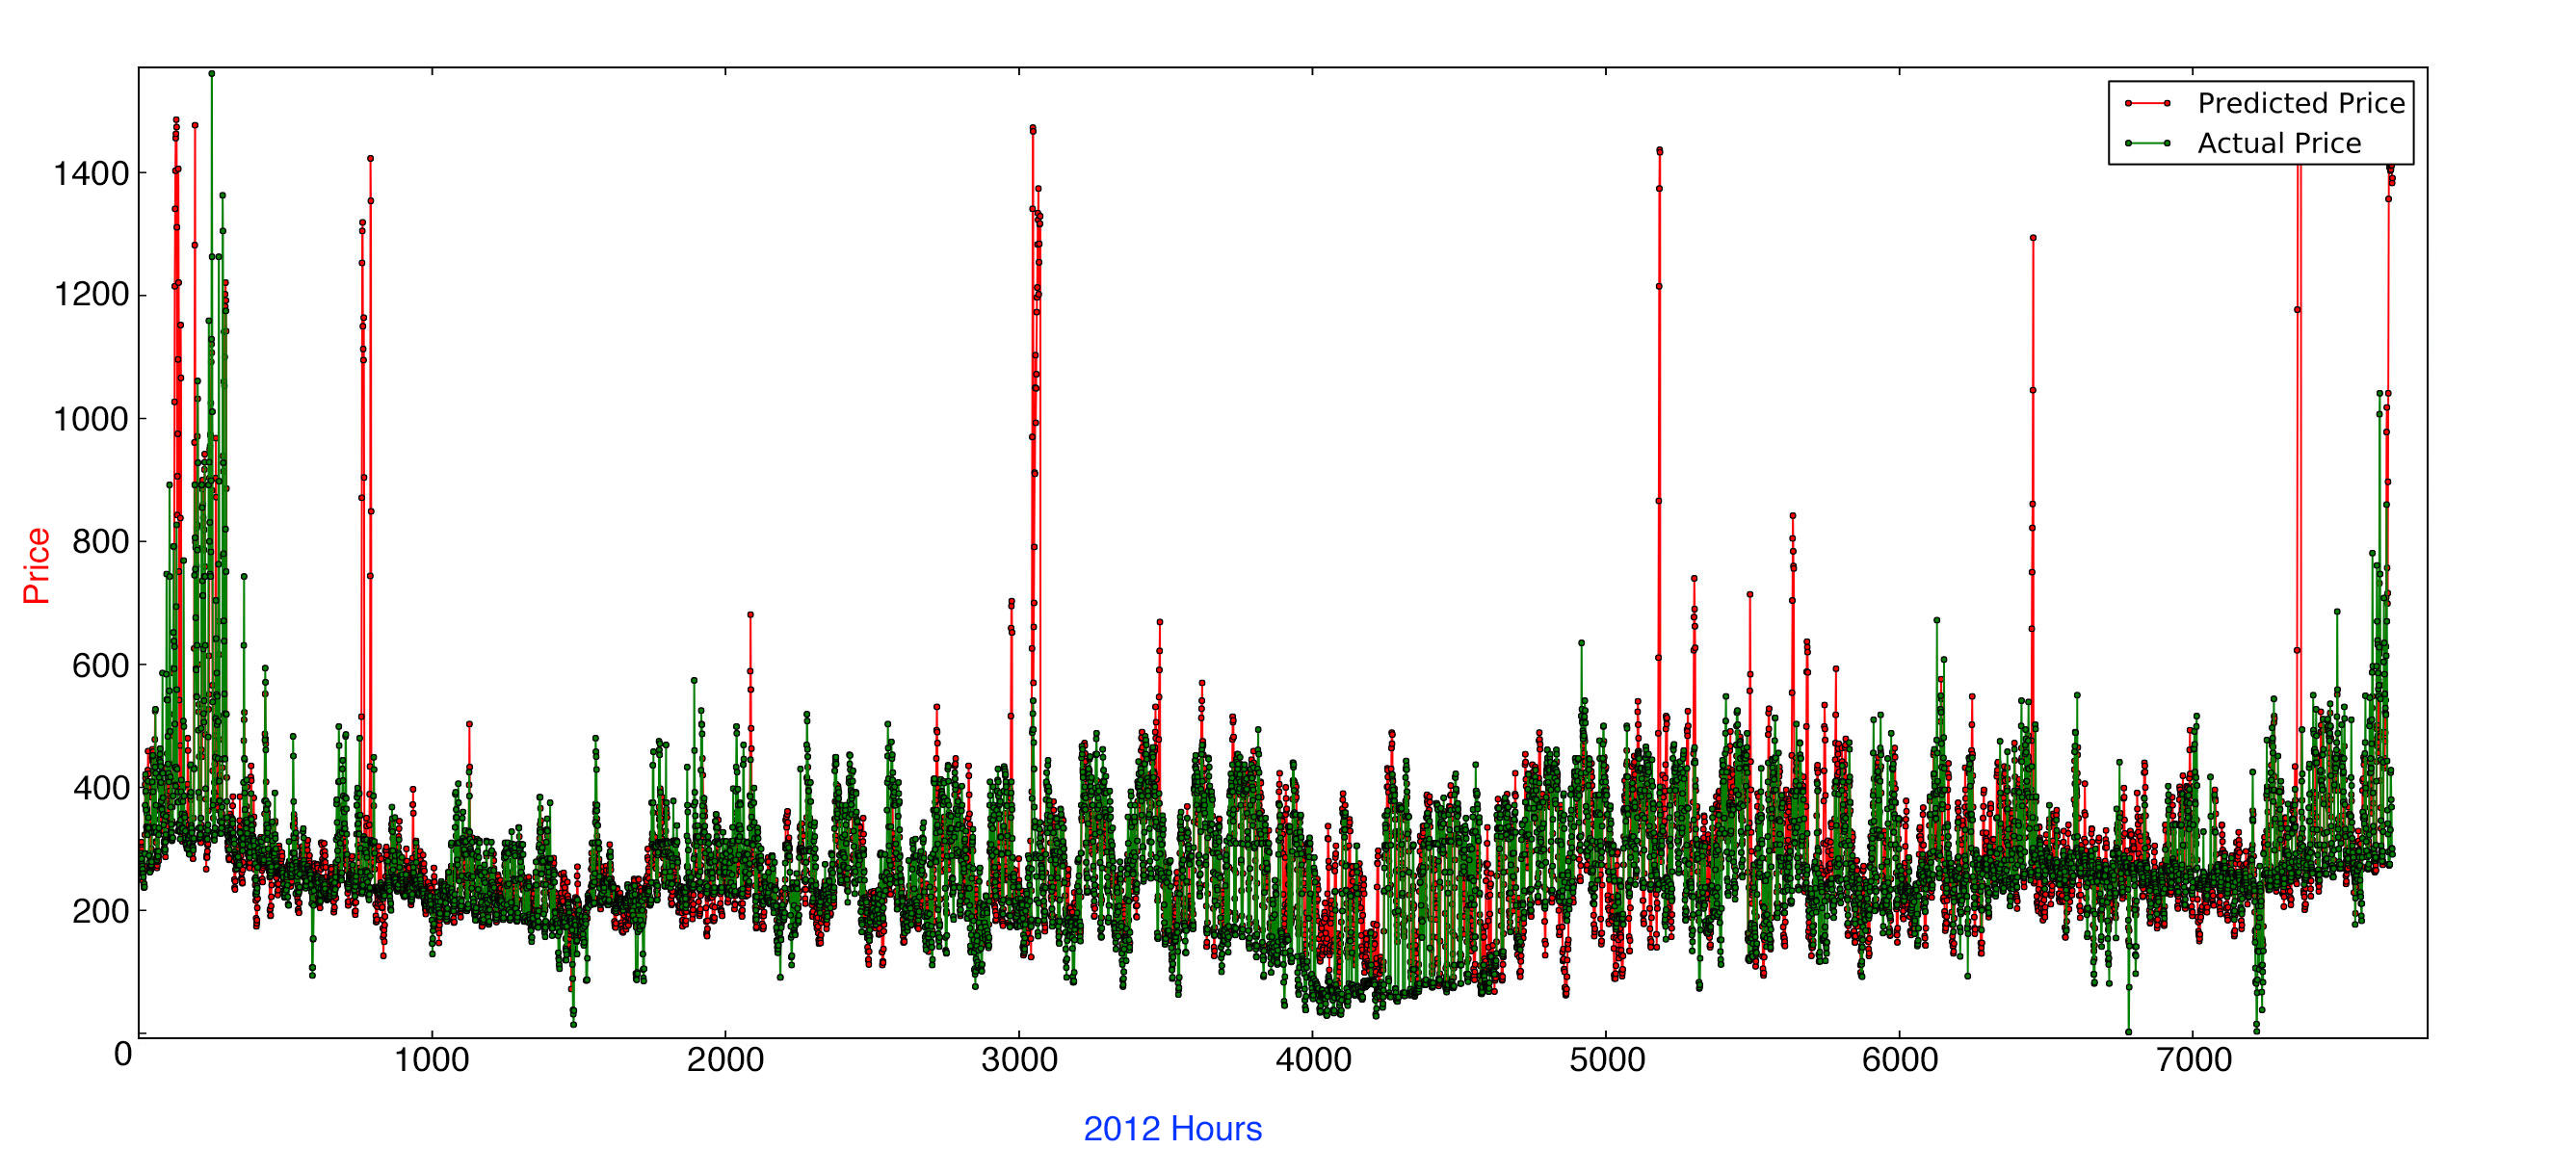
\includegraphics[width=\linewidth]{billeder/PriceExperimentalAnalysis/NoTrimming.png}
\caption{The \#1 forecast with no trimming of the dataset}
\label{fig:NoTrim}
\end{figure}

If we take a look at the same dataset but this time with a 1\% high and low trim (2\% in total) in figure~\ref{fig:1PTrim}; we clearly see that the actual prices in the beginning aren't spiking as heavily as they did in figure~\ref{fig:NoTrim}. This of course prevents us from predicting these high spikes but if we take a look at the rest of the set we see that the 5 faulty spikes have gone as well. This shows the trade off between being able to predict the outliers and the errors they introduce.

\begin{figure}[H]
\centering
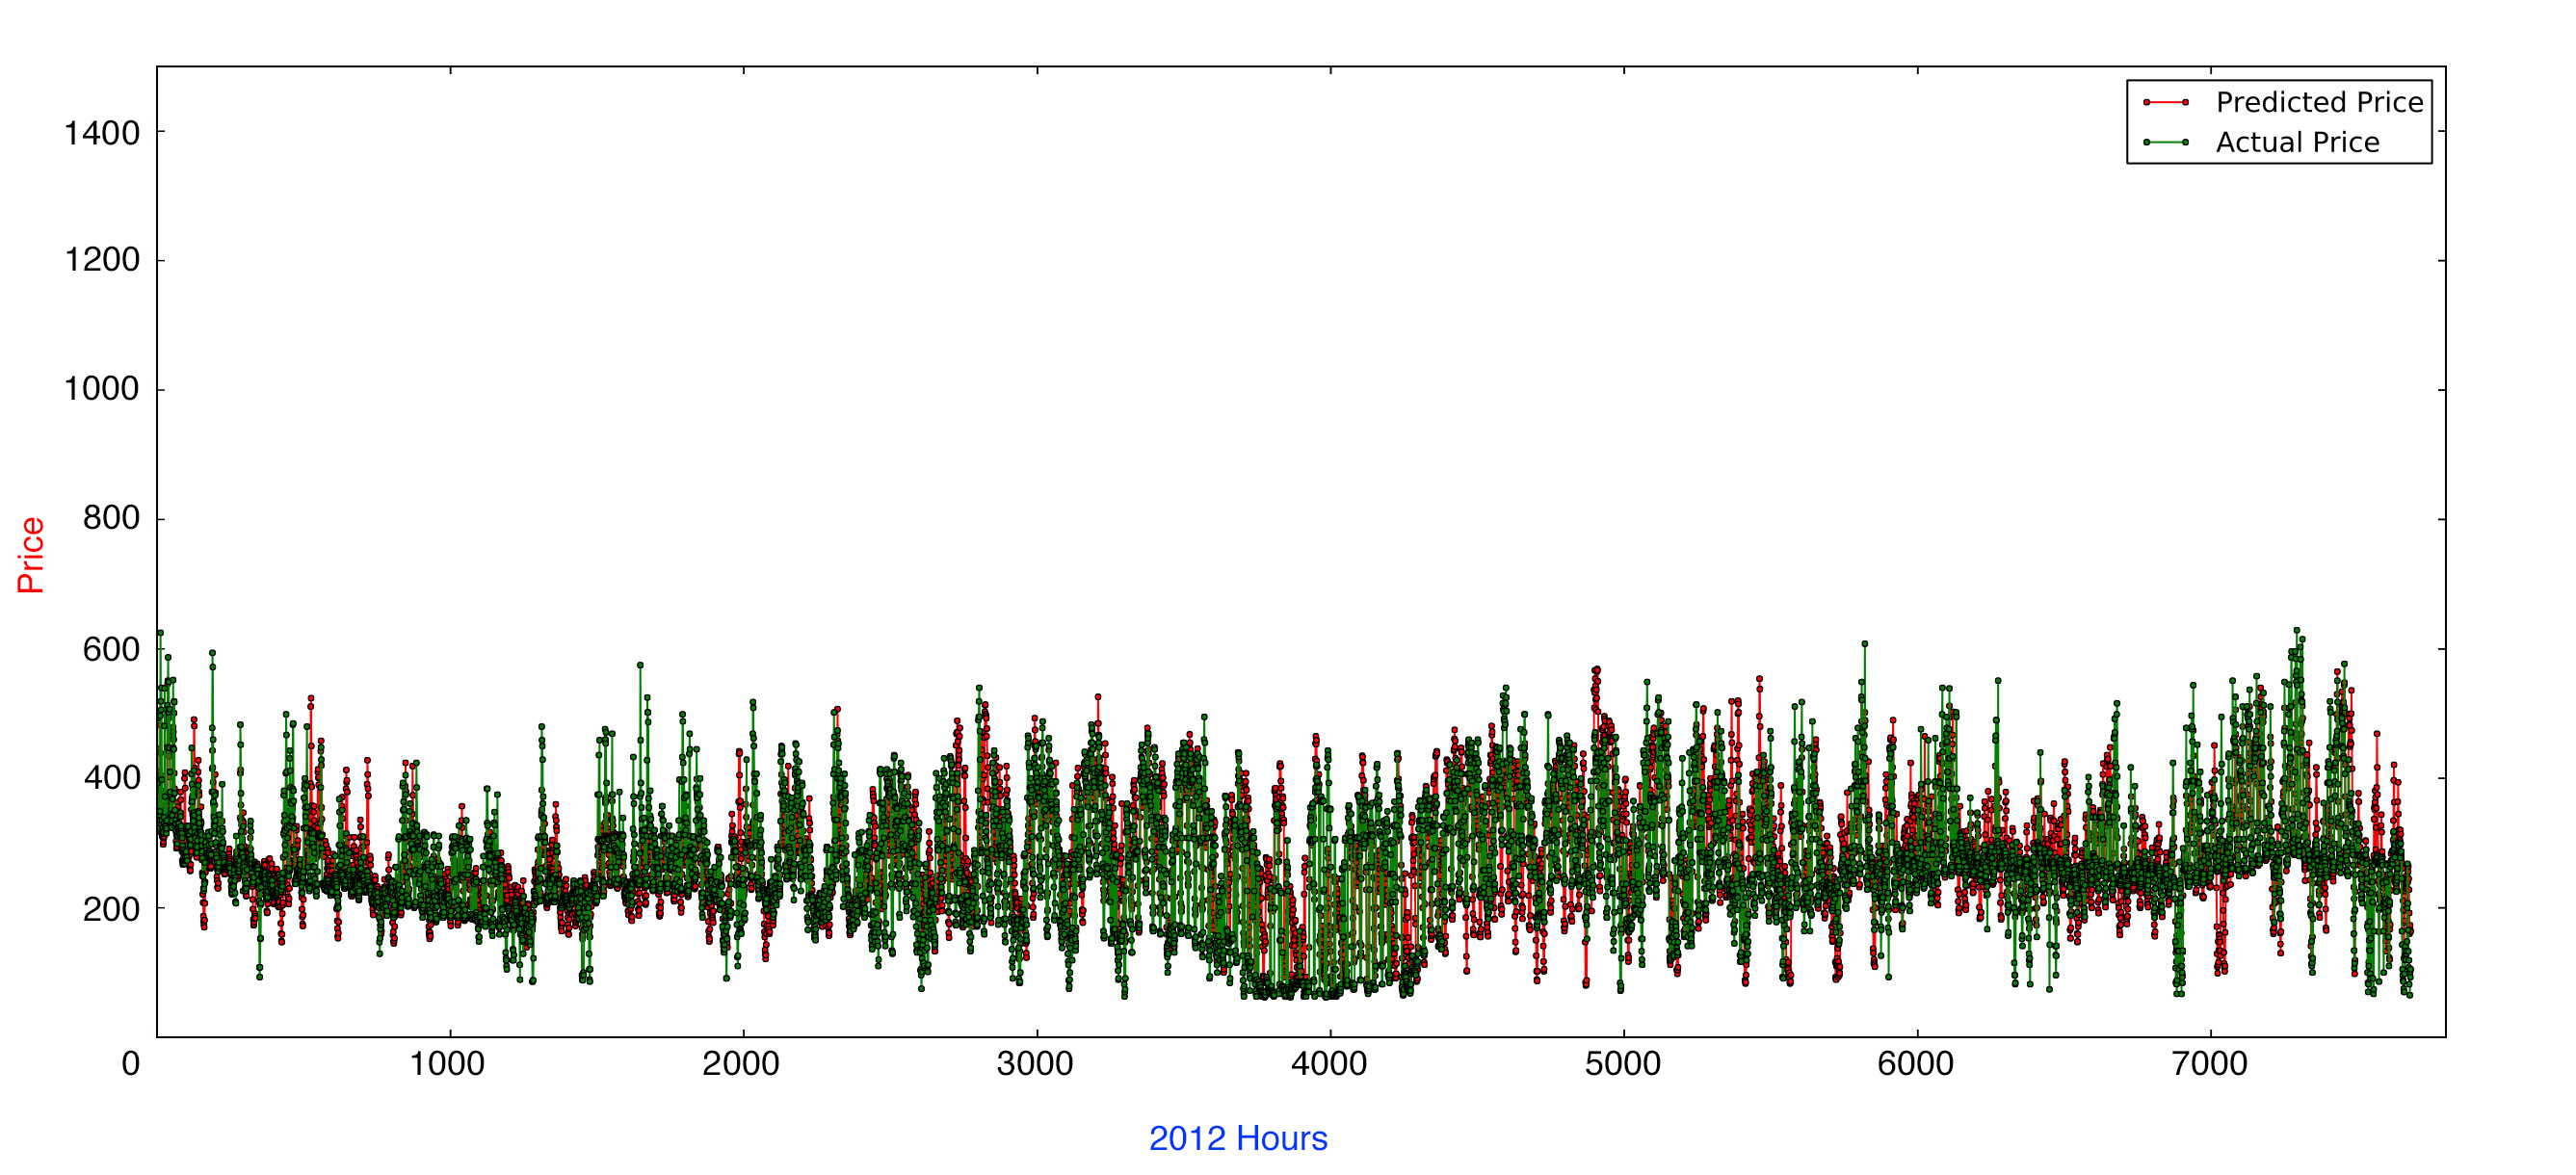
\includegraphics[width=\linewidth]{billeder/PriceExperimentalAnalysis/1PTrim.png}
\caption{The \#1 forecast with 1\% trimming in both ends of the dataset}
\label{fig:1PTrim}
\end{figure}

In figure~\ref{fig:AllTrims} we see the dataset from figure~\ref{fig:1PTrim} with 1\% trim. The lines shows how much would be cut of if we applied 2\%(Purple), 3\%(Red), 4\%(Black) and 5\%(Blue) trimming. Here we clearly see that it is removing data - that is part of the norm - from the set. With every percent we go up we remove 363 entries so at 5\% trim (top and bottom) we will be removing 1815 entries from our dataset. This will result in us never being able to predict values higher or lower than the bars. We are of course not interested in that as most of the values we trim from 2\% and up are part of a more normalized dataset. Also the improvements we see from 1\% trim to 5\% trim is 12.97\% which is pretty insignificant compared to the 1815 cases that we will be unable to predict.

\begin{figure}[H]
\centering
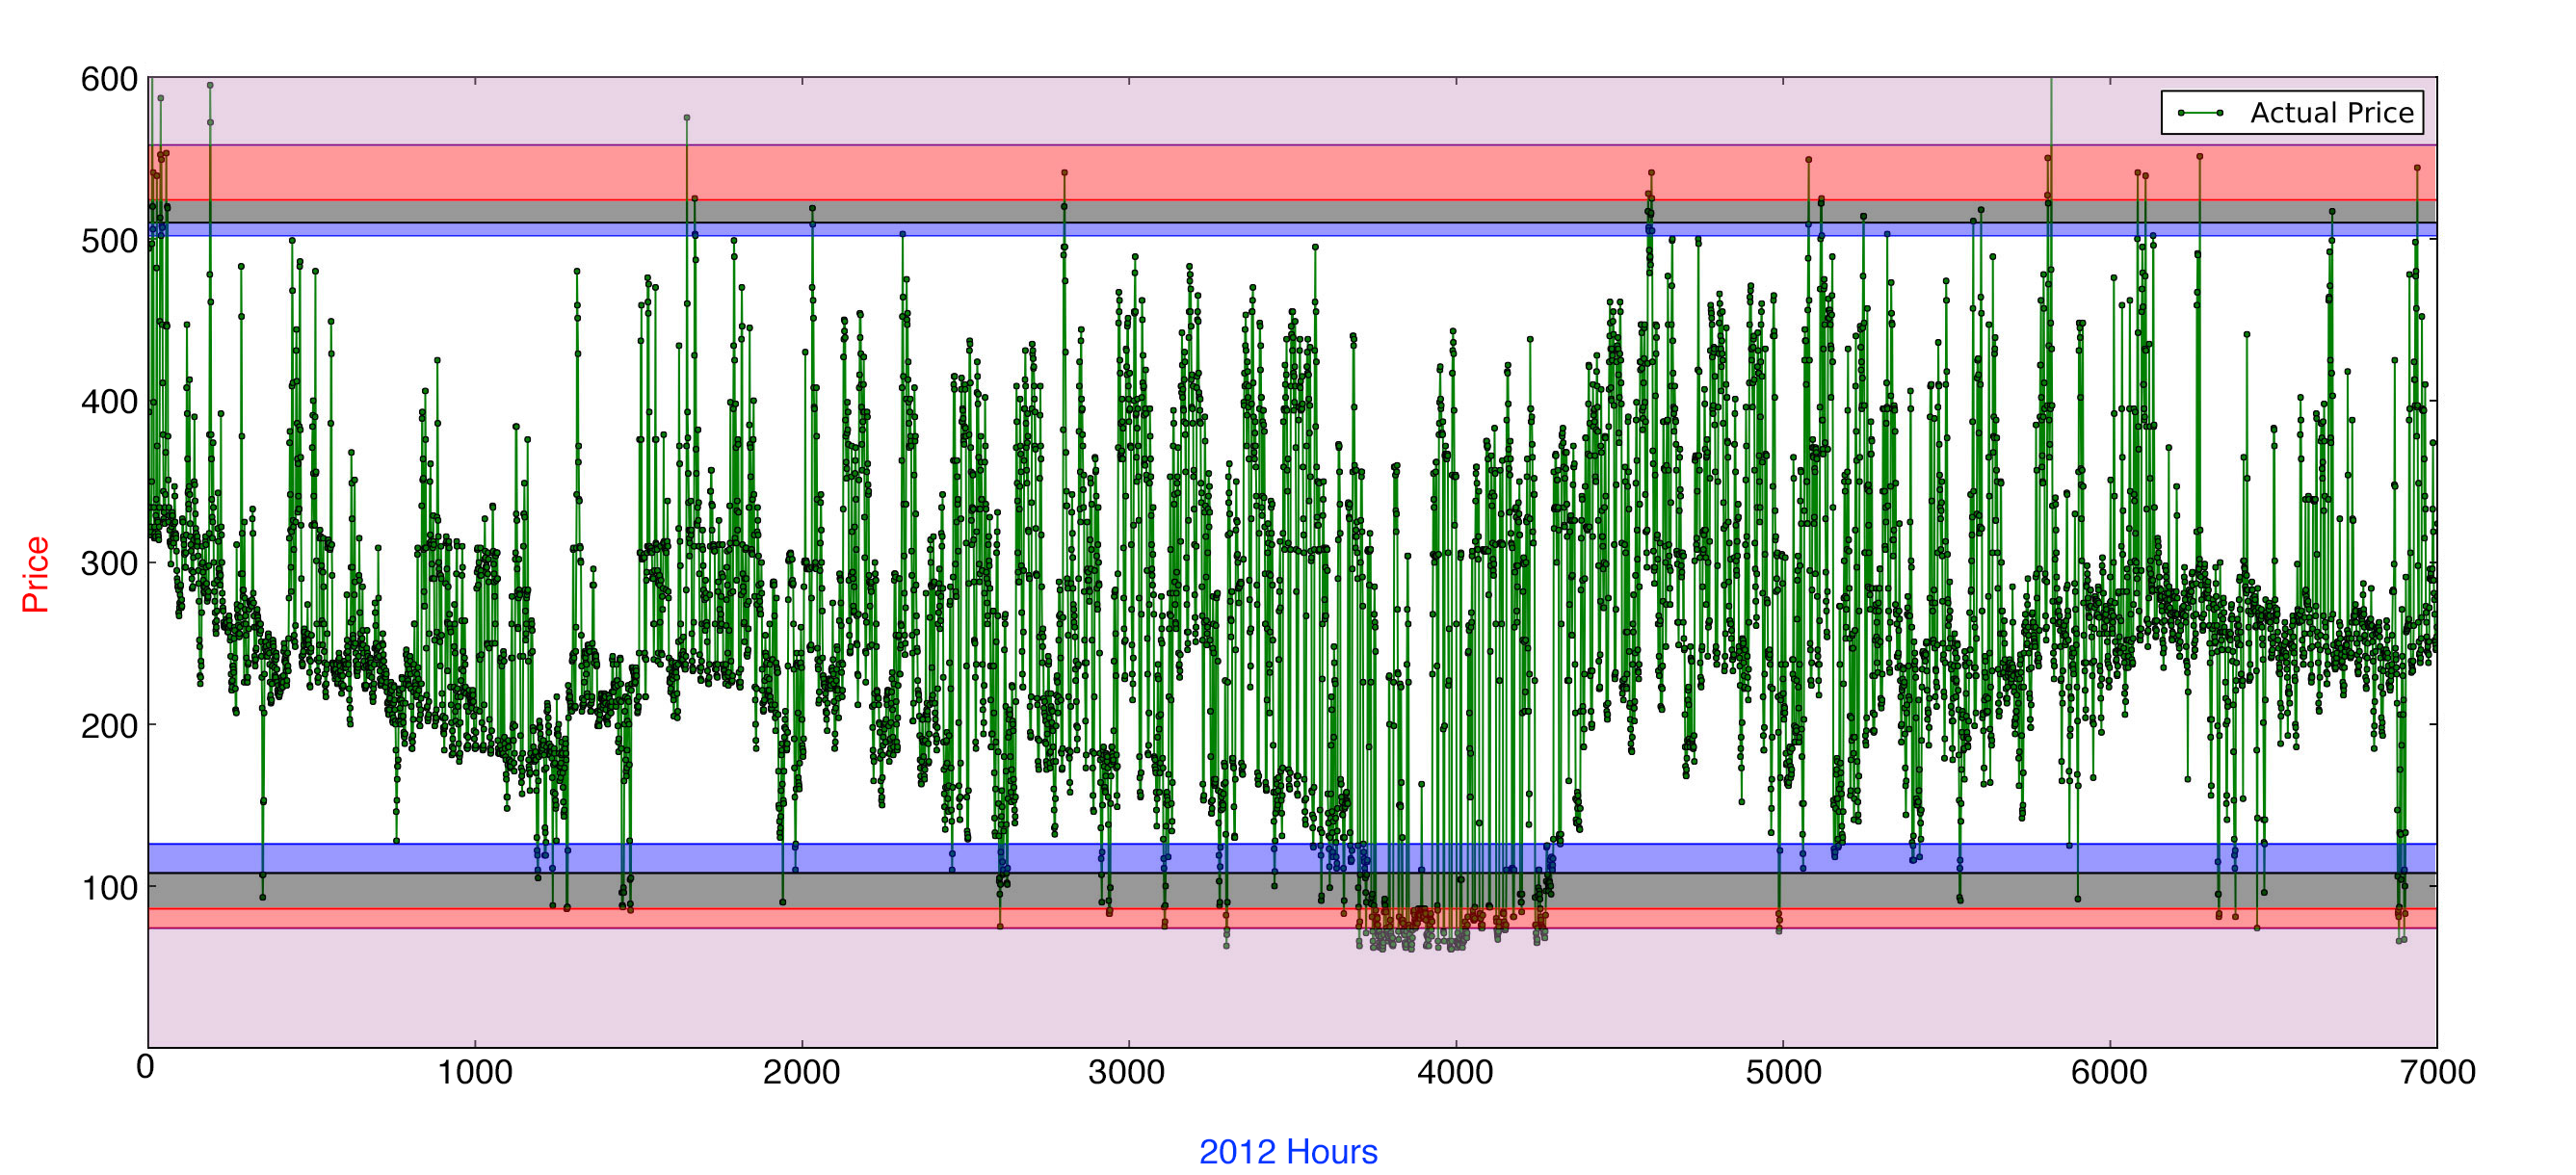
\includegraphics[width=\linewidth]{billeder/PriceExperimentalAnalysis/restOfTrims.png}
\caption{The \#1 forecast with 2\%(Purple), 3\%(Red), 4\%(Black) and 5\%(Blue) trimming in both ends of the dataset}
\label{fig:AllTrims}
\end{figure}

\todo{Skriv om tabellen. Vis sammenhaeng i forhold til 1815 entries vil mistes paa baggrund af en forbedring paa kun 8 MAE i bedste tilfaelde.}


\begin{table}[H]
\centering  % used for centering table
\resizebox{0.6\textwidth}{!}{
	\begin{tabular}{|c|c|c|c|c|c|} % centered columns (7 columns)
	\hline
	1PTrim & 2PTrim & 3PTrim & 4PTrim & 5PTrim & Number\\ [0.5ex] % inserts table 
	\hline                  % inserts single horizontal line
	47,21 & 42,90 & 44,48 & 42,46 & 41,79 & \#1  \\ \hline
	46,15 & 43,67 & 43,07 & 39,16 & 40,28 & \#2  \\ \hline
	47,14 & 45,10 & 43,38 & 40,50 & 39,41 & \#3  \\ \hline
	46,70 & 43,96 & 43,21 & 40,03 & 40,29 & \#4  \\ \hline
	45,96 & 43,25 & 45,51 & 40,74 & 40,42 & \#5  \\ \hline
	47,27 & 45,96 & 44,98 & 41,39 & 39,98 & \#6  \\ \hline
	45,93 & 44,66 & 43,39 & 41,02 & 40,40 & \#7  \\ \hline
	46,64 & 42,69 & 44,48 & 41,69 & 40,61 & \#8  \\ \hline
	45,98 & 44,51 & 43,71 & 40,74 & 41,08 & \#9  \\ \hline
	45,60 & 46,07 & 45,81 & 42,52 & 41,32 & \#10 \\ \hline
	\end{tabular}
}
\caption{Trims} % title of Table
\label{table:Top10Trimming} % is used to refer this table in the text
\end{table}

\subsubsection{Conclusion}
In this experiment we saw how trimming can positively affect the predictions. We also discussed the trade offs in the trimming procedure as we lowered the possible outcomes of our predictions. This is a balance between improvement and the amount of prices we will not be able to predict. The 1\% trim showed us an improvement of 20.99\% and removed some extreme failed predictions where the ANN would overshoot the target by 800+. We also learned that higher trimming rates did not really improve the results very much thus making it easy for us to decide on a trimming rate of 1\%.

\newpage
\subsection{Experiment three: Calculated inputs}
\label{sec:priceExperimentThree}
This experiment was conducted to test the different calculated inputs that we described in section~\ref{sec:stratsForPrediction}. This includes Slope calculation, Skewness, EWMA - Historical Volatility and Scatter. We took the three best results from experiment one and ran every combination of the calculated inputs on the best results. The experiment was conducted on the 1\% trimmed version of the 3 best results from experiment one - due to the improvements seen in experiment two. Also we did a test on the most basic dataset we had available: Price and Consumption with no trimming. This was done to validate the impact of the different strategies before applying any other factors to the prediction.

\subsubsection{Hypothesis}
In this experiment we applied different calculated inputs to the neural network. This was done to give some knowledge about the prior trend when trying to predict the next 24 hours. This experiment is expected to show an improvement in the curve fitting thus giving us a better MAE.

Also we conducted a trial to test the effect of these strategies on a vanilla dataset(Consumption and last know price with no trim) and we expect these predictions to improve a good deal with strategies applied thus making up for some of the other factors not included e.g. Wind Speed, Temperature, Time of Day etc.

\subsubsection{Variables}
In this experiment we had 4 variables that we tested:
\begin{itemize}
	\item Slope calculation (Slope)
	\item Skewness (Skew)
	\item EWMA - Historical Volatility (EWMA)
	\item Scatter (Scatter)
\end{itemize}

The setup of the different strategies have been tested on the best result from experiment one.

\subsubsection{EWMA}
The EWMA is used to calculate the volatility of the curve. The electricity price is highly volatile and therefore we anticipate that knowledge about the historical volatility will help the predictions. In the EWMA we have a smoothing factor which indicates how sensitive the strategy will be towards fluctuations in the curve. A lower smoothing factor will allow for more rapid changes and vice versa. In table ~\ref{table:SmoothingFactorTest} we see that the best result is a smoothing factor of 0.9 and a stack size of 16.
\todo{Skriv i forhold til stack size}

\begin{table}[H]
\centering  % used for centering table
\resizebox{0.5\textwidth}{!}{
	\begin{tabular}{|c|c|c|c|c|} % centered columns (7 columns)
	\hline
	Rank & Stack size & Smoothing factor & MAE & \% ranking \\ [0.5ex] % inserts table 
	\hline                   % inserts single horizontal line
	1 & 16 & 0,9 & 45,96 & - \\ \hline
	2 & 12 & 0,1 & 46,13 & 0,38\% \\ \hline
	3 & 20 & 0,9 & 46,47 & 1,11\% \\ \hline
	4 & 8 & 0,9 & 46,55 & 1,28\% \\ \hline
	5 & 20 & 0,5 & 46,56 & 1,31\% \\ \hline
	6 & 24 & 0,4 & 46,58 & 1,36\% \\ \hline
	7 & 20 & 0,7 & 46,59 & 1,37\% \\ \hline
	8 & 12 & 0,9 & 46,61 & 1,41\% \\ \hline
	9 & 24 & 0,8 & 46,78 & 1,79\% \\ \hline
	10 & 24 & 0,5 & 46,88 & 2,0\% \\ \hline
	\end{tabular}
}
\caption{Smoothing factor test} % title of Table
\label{table:SmoothingFactorTest} % is used to refer this table in the text
\end{table}

\subsubsection{Skewness}
The skewness denotes whether an observation falls to the left or the right of the median as described in section~\ref{sec:skewness}. This is used to determine in what direction the graph is currently moving thus giving us information about the trend. We experimented with how many historical prices we had to include in the calculation of the skewness and ended up with 4 being the best even though they are very close.

\begin{table}[H]
\centering  % used for centering table
\resizebox{0.5\textwidth}{!}{
	\begin{tabular}{|c|c|c|} % centered columns (7 columns)
	\hline
	Skewness stack & MAE & \% ranking \\ [0.5ex] % inserts table 
	\hline                  % inserts single horizontal line
	4  & 45,09 & -\\ \hline
	2  & 45,15 & 0,13\%\\ \hline
	6  & 45,69 & 1,33\%\\ \hline
	20 & 46,05 & 2,12\%\\ \hline
	8  & 46,14 & 2,32\%\\ \hline
	24 & 46,16 & 2,37\%\\ \hline
	16 & 46,47 & 3,06\%\\ \hline
	12 & 46,66 & 3,48\%\\ \hline
	\end{tabular}
}
\caption{Number of historical prices to include in the skewness calculation} % title of Table
\label{table:SkewnessTest} % is used to refer this table in the text
\end{table}

\subsubsection{Slope calculation}
The slope calculation is conducted to tell us something about the gradient of the current curve as described in section~\ref{sec:curveAnalysis}. We examine here how many historical prices should be included in the curve gradient analysis to say something about what direction (up, down or steady) the curve is heading. The test shows us that a stack size of 4 prices is the best but again they are not differing much.

\begin{table}[H]
\centering  % used for centering table
\resizebox{0.5\textwidth}{!}{
	\begin{tabular}{|c|c|c|} % centered columns (7 columns)
	\hline
	Slope stack & MAE & \% ranking \\ [0.5ex] % inserts table 
	\hline                  % inserts single horizontal line
	4  & 45,72 & - \\ \hline
	12 & 46,05 & 0,71\%\\ \hline
	6  & 46,09 & 0,81\%\\ \hline
	2  & 46,31 & 1,29\%\\ \hline
	16 & 46,67 & 2,01\%\\ \hline
	24 & 46,76 & 2,27\%\\ \hline
	20 & 46,87 & 2,52\%\\ \hline
	8  & 47,81 & 4,57\%\\ \hline
	\end{tabular}
}
\caption{Slope calculation stack size} % title of Table
\label{table:CurveTest} % is used to refer this table in the text
\end{table}

\subsubsection{Results}
We ran 3 experiments reflecting the top 3 results from experiment one. Before the results of the experiments we list the input parameters that we use the strategies on. 

Variables: Price, Consumption, Wind Speed, Temperature, Time of Day (Matrix), Day of Week (Matrix) and Season of Year (Matrix)
\begin{table}[H]
\centering  % used for centering table
\resizebox{0.7\textwidth}{!}{
	\begin{tabular}{|c|c|c|c|c|c|c|} 
	\hline
	Rank & Curve & Skew & EWMA & Scatter & MAE & \% ranking\\ [0.5ex] % inserts table 
	\hline                  % inserts single horizontal line
	1  &       & \x    & \x    &       & 45,35 & - \\ \hline
	2  & \x    & \x    & \x    &       & 45,76 & 0,91\% \\ \hline
	3  & \x    &       &       & \x    & 45,83 & 1,06\% \\ \hline
	4  & \x    &       &       &       & 46,10 & 1,66\% \\ \hline
	5  & \x    & \x    &       &       & 46,40 & 2,32\% \\ \hline
	6  & \x    &       & \x    &       & 46,47 & 2,48\% \\ \hline
	7  &       & \x    &       &       & 46,53 & 2,6\% \\ \hline
	8  &       &       & \x    &       & 46,53 & 2,61\% \\ \hline
	9  &       &       & \x    & \x    & 46,72 & 3,03\% \\ \hline
	10 &       &       &       & \x    & 46,88 & 3,38\% \\ \hline
	11 & \x    & \x    & \x    & \x    & 47,40 & 4,54\% \\ \hline
	12 &       & \x    &       & \x    & 47,65 & 5,09\% \\ \hline
	13 & \x    &       & \x    & \x    & 47,82 & 5,46\% \\ \hline
	14 & \x    & \x    &       & \x    & 47,96 & 5,76\% \\ \hline
	15 &       & \x    & \x    & \x    & 48,45 & 6,83\% \\ \hline
	\end{tabular}
}
\caption{Statistical results} % title of Table
\label{table:Statistical1} % is used to refer this table in the text
\end{table}

The first run shown in table~\ref{table:Statistical1} shows no big improvements between the different strategies but neither do they show an improvement compared to the results from experiment two - this combination gave us 47,21 in MAE. Compared to the best result from table~\ref{table:Statistical1} that is only an improvement of 4.10\%.

\begin{figure}[H]
\centering
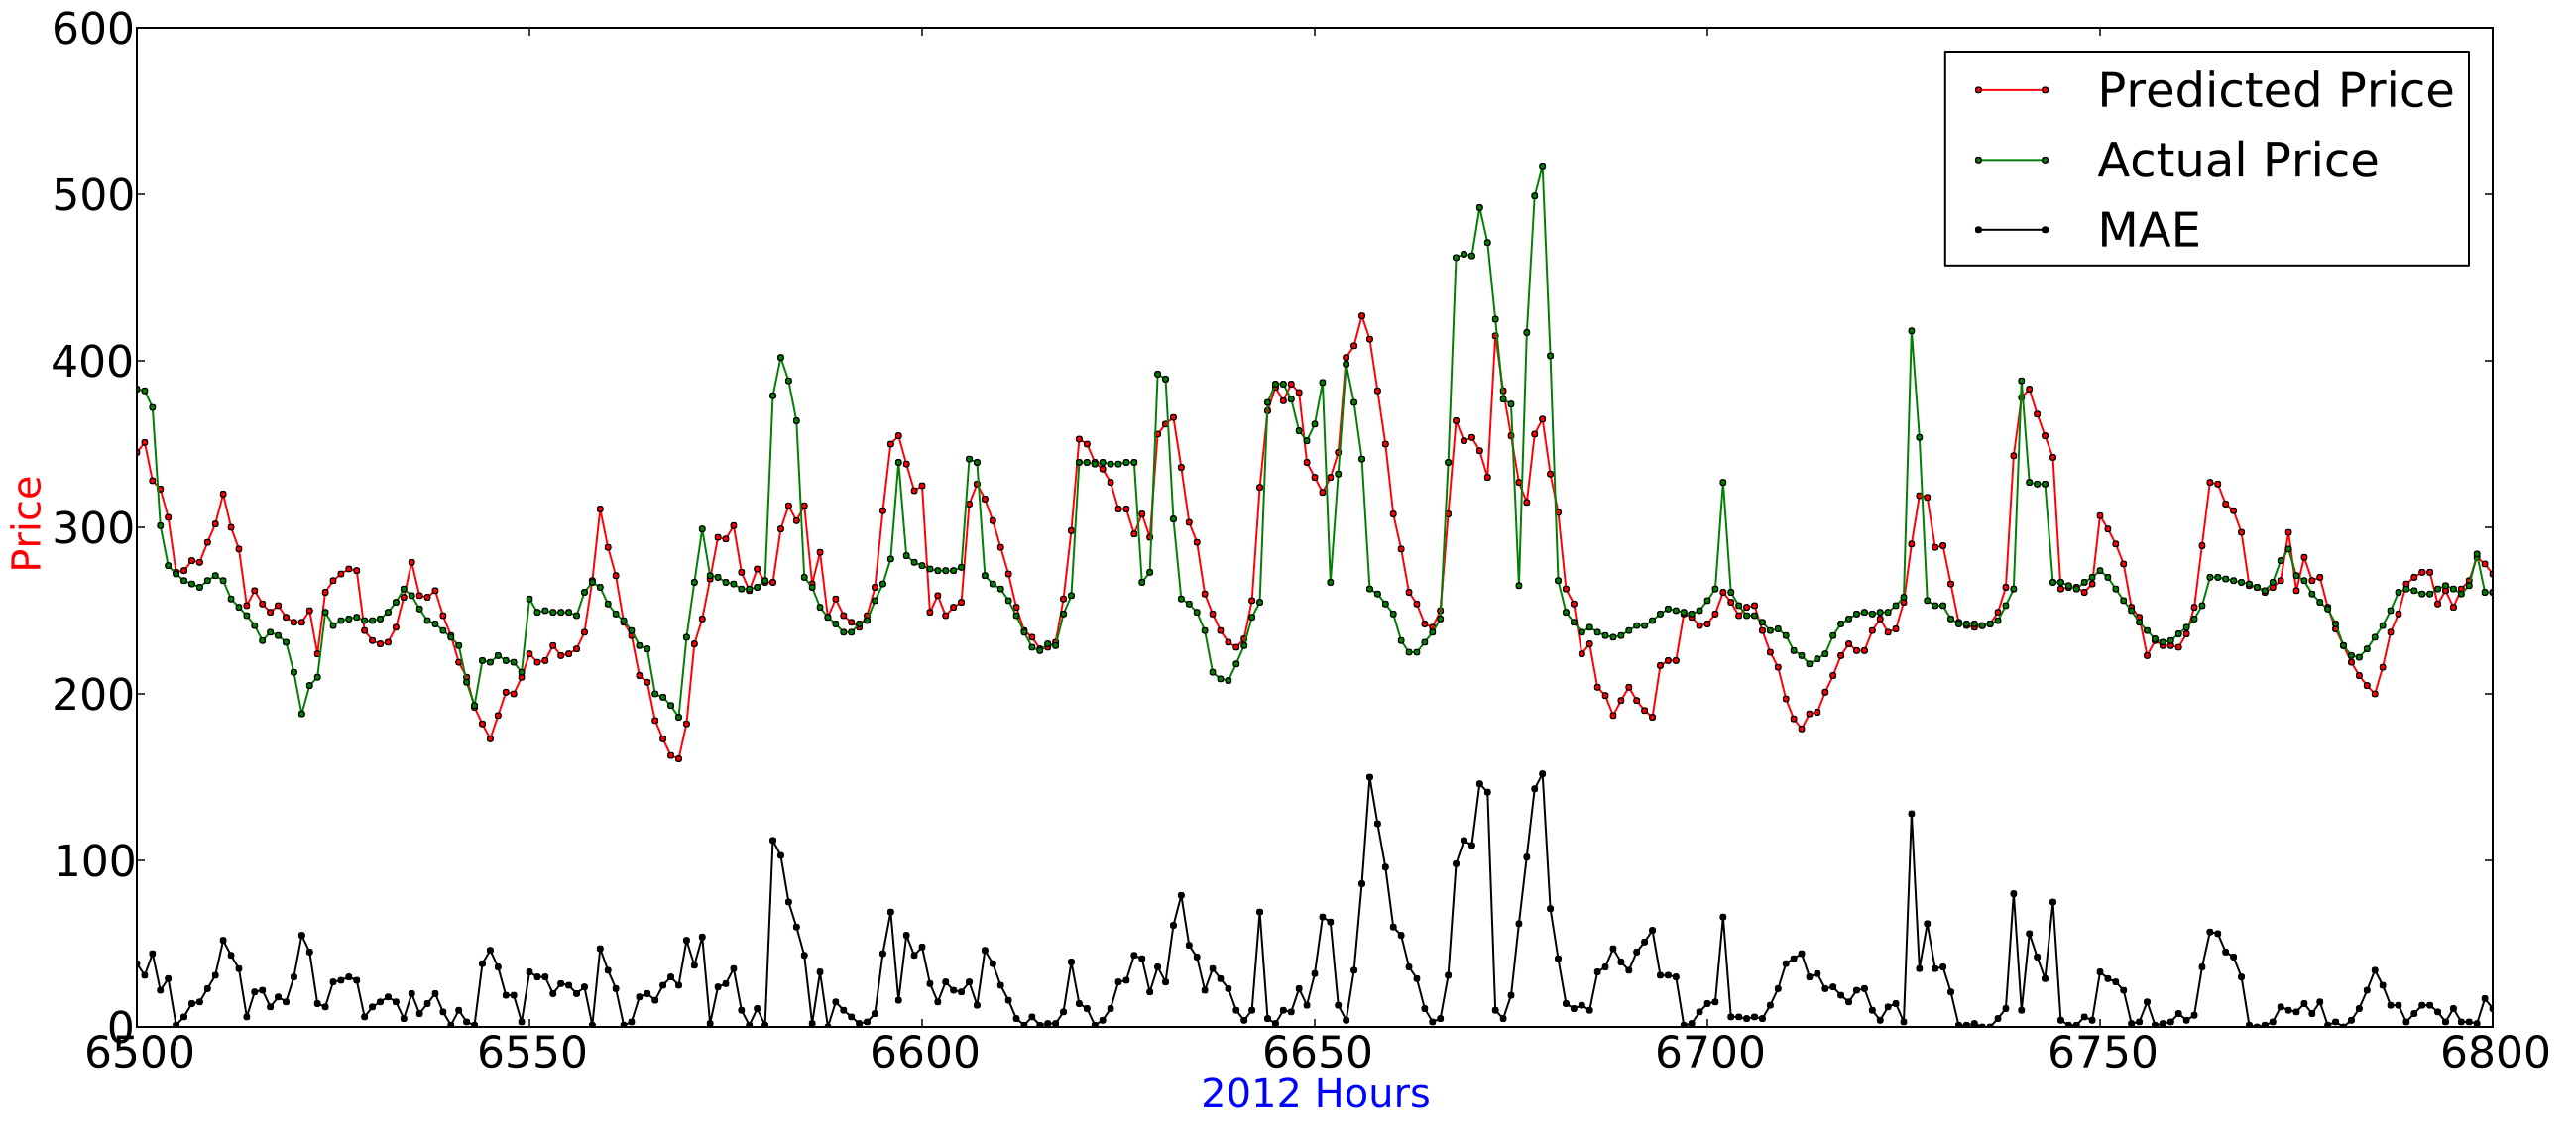
\includegraphics[width=\linewidth]{billeder/PriceExperimentalAnalysis/X3_Nr1_Best_skew_historical.png}
\caption{\#1 forecast from experiment three. Shows how well it follows the curve. The black curve in the bottom is the error for each prediction.}
\label{fig:X3_Best_With_MAE}
\end{figure}

In figure~\ref{fig:X2_X3_3800_4000} we see how the ANN has trouble predicting the unusual low values. This is the same for the experiment two prediction as it is for the experiment three prediction. The case we see in figure~\ref{fig:X2_X3_3800_4000} is what we hoped the calculated inputs would help the ANN to be better at predicting; since it has gained some knowledge about the immediate past. Experiment three also introduces more jagged curves where it fluctuates up and down a lot compared to the prediction from experiment two - which has smoother curves. This is because of the calculated inputs that add values that are interpreted into either a rising or a falling curve. Compared to the prediction from experiment two it does not have this knowledge and only relies on the interaction between the quantifiable parameters from experiment one.

If we apply all of the calculated inputs to the prediction we get figure~\ref{fig:X2_X3_AllParameters_3800_4000}. In this figure we can see that it actually is able to drop to the lowest values in the dataset. On the other hand it has trouble rising from the low values which reintroduces the error but in the top of the dataset. This is due to the fact that with all applied calculated inputs it will follow the curve better but at the same time the historical trend of the curve has to great of an influence on the predictions thus making it unable to rise/fall fast enough to follow the curve.

Another problem with the calculated inputs are that making predictions with an ANN is about generalizing the inputs to reflect a mathematical function. If the ANN does not see enough examples of the calculated inputs throughout the training dataset it will not be able to make this generalization and thus not be able to use it efficiently in the predictions of the next 24 hours. If the first prediction in the next 24 hours is wrong (compared to the ideal prices) the calculated inputs can help elevate/decrease the error since the last known price is added to the calculation of these features(This can be seen in figure~\ref{fig:X2_X3_3816_3840} and in ~\ref{fig:X3_Price_Consump_Worst}). Also the calculated inputs are more or less unique throughout the whole year since the price does not follow a specific pattern that makes it harder to generalize the calculated inputs in the price prediction. \todo{Print alle values omkring calculated inputs. Sammenhold dem med price og andre parametre og se om der er en tendens eller om det er totalt random. Dataset analysis}

\todo{Calculated inputs skal staa i forhold til Scatter. Scatter goer den det selv. Calculated der hjaelper vi den.}

The results in table~\ref{table:Statistical2} and ~\ref{table:Statistical3} are control groups to show that it is not a single combination that has no benefit from the calculated inputs and that other combinations does not benefit from them either.

\begin{figure}[H]
\centering
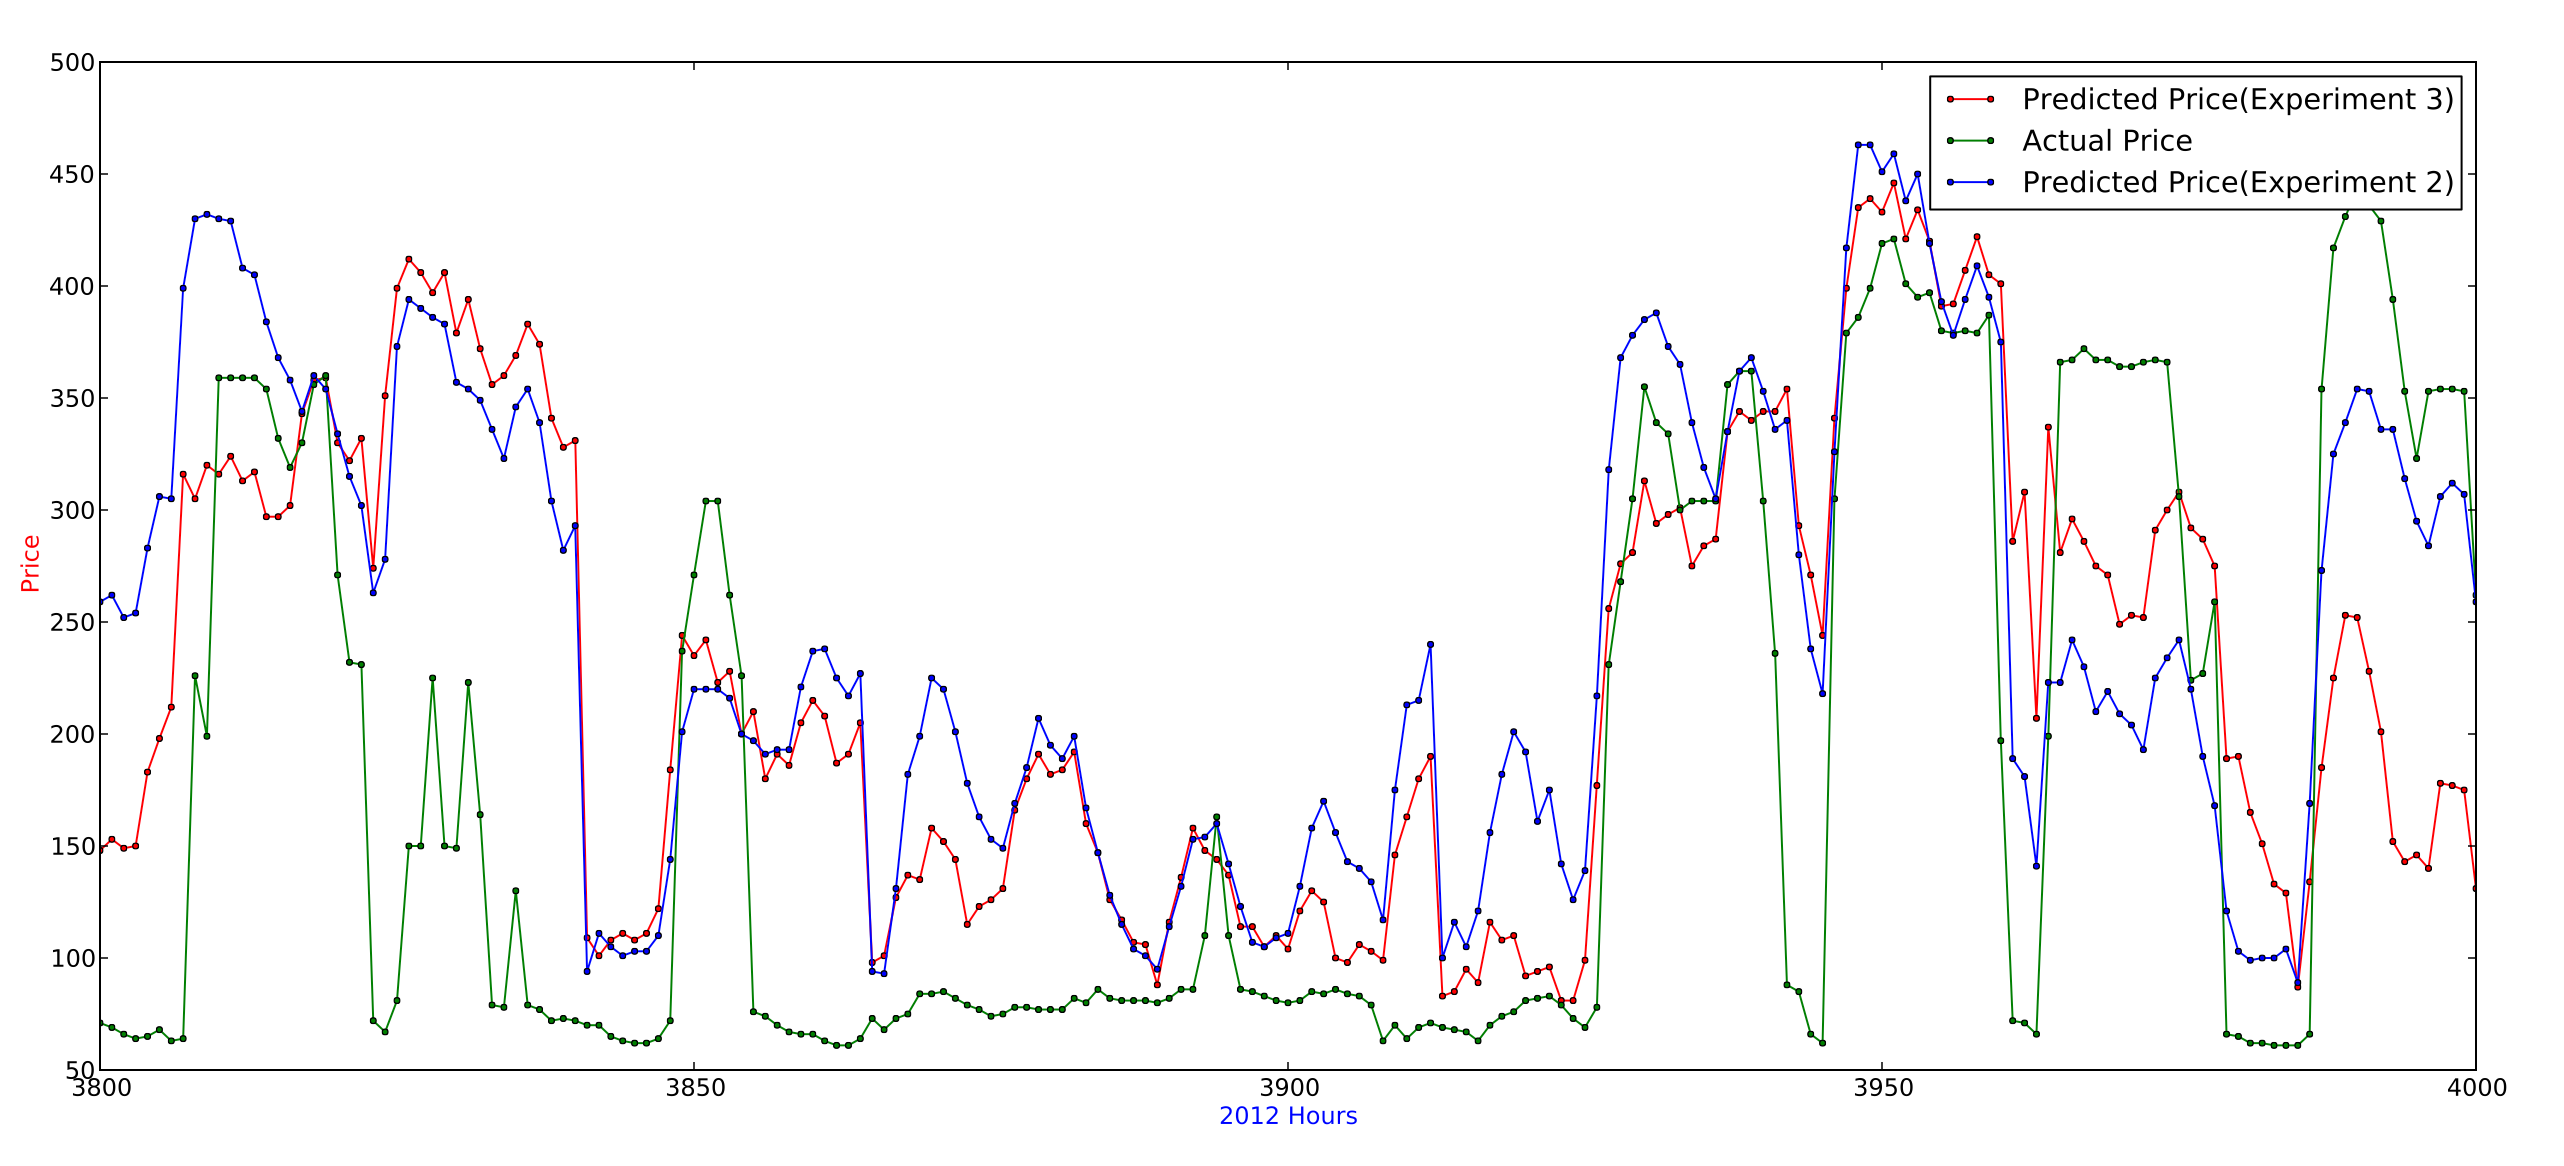
\includegraphics[width=\linewidth]{billeder/PriceExperimentalAnalysis/X2_X3_3800_4000.png}
\caption{A comparison of \#1 forecast from experiment two and three. This segment is from the middle of the year. (Skew, EWMA)}
\label{fig:X2_X3_3800_4000}
\end{figure}

\begin{figure}[H]
\centering
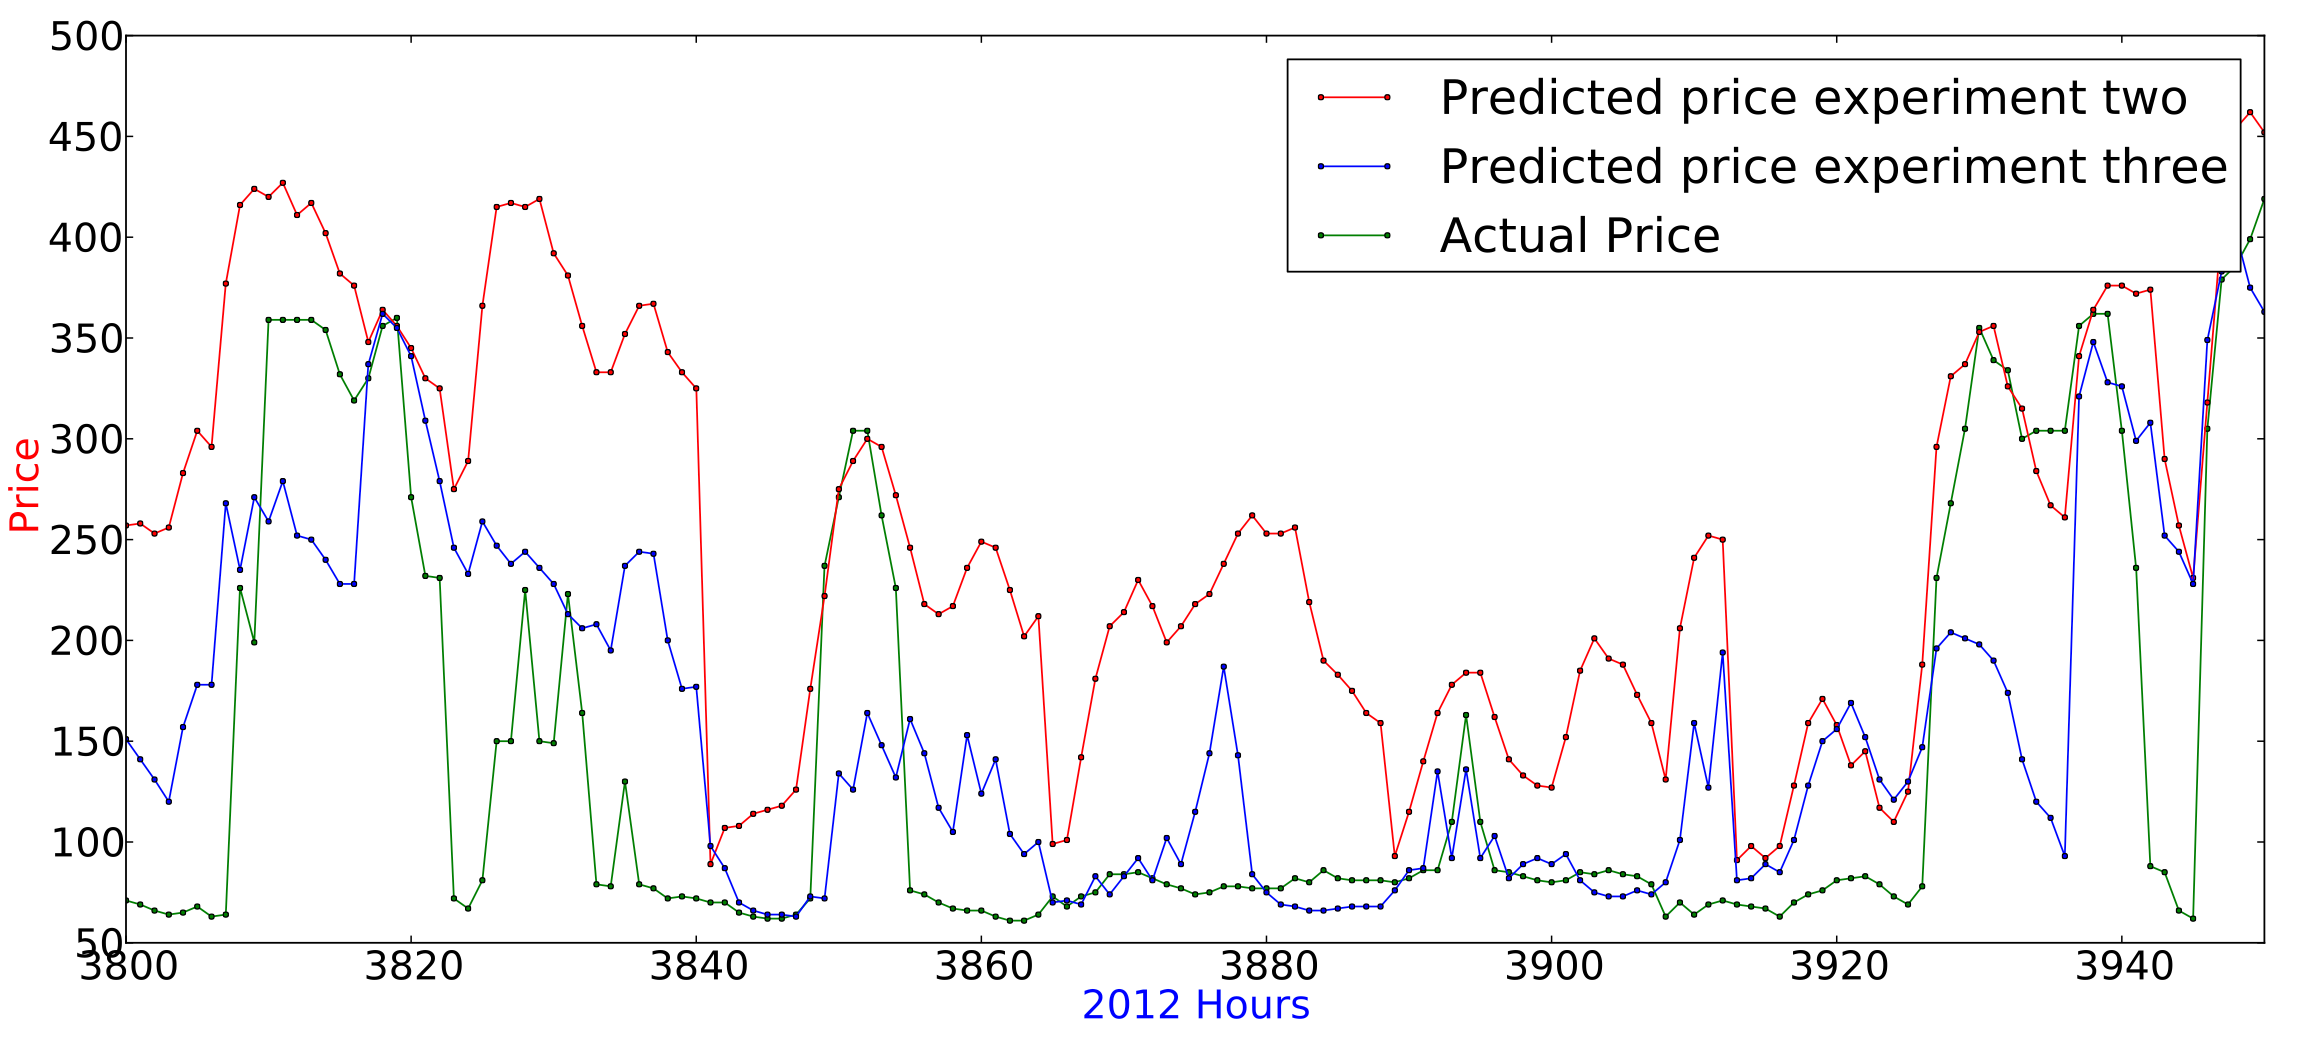
\includegraphics[width=\linewidth]{billeder/PriceExperimentalAnalysis/X2_X3_AllFeatures_3800_4000.png}
\caption{A comparison of \#1 forecast from experiment two and three. This segment is from the middle of the year. All features applied(Skew, Curve, EWMA, Scatter).}
\label{fig:X2_X3_AllParameters_3800_4000}
\end{figure}

\begin{figure}[H]
\centering
\begin{subfigure}{.5\textwidth}
  \centering
	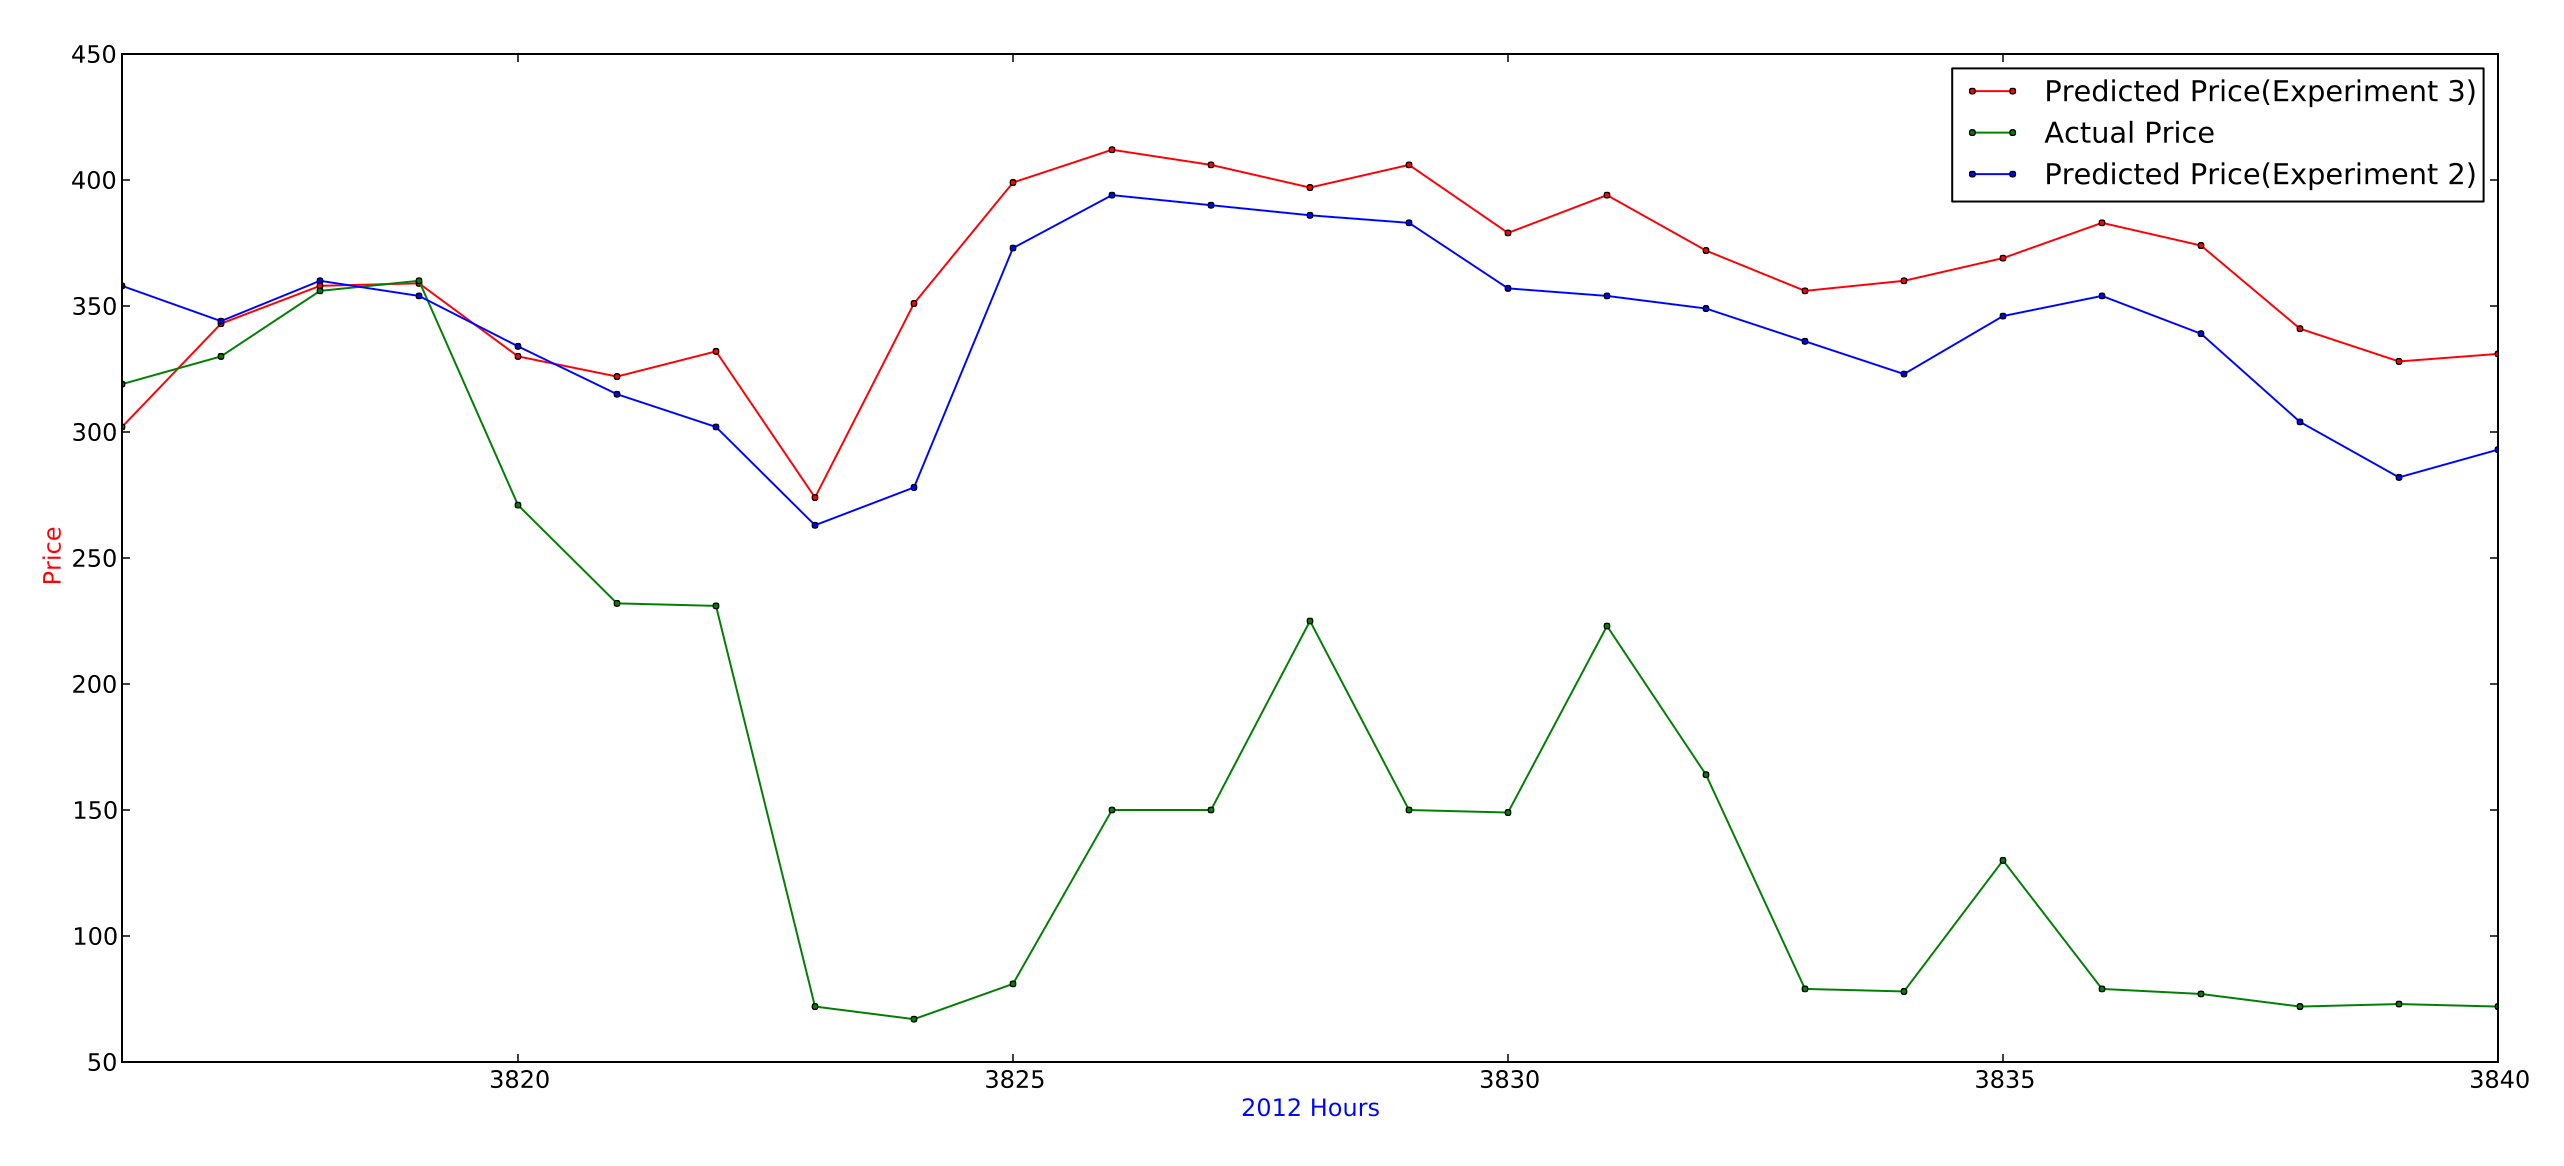
\includegraphics[width=\linewidth]{billeder/PriceExperimentalAnalysis/X2_X3_3816_3840.png}
	\caption{A comparison of \#1 forecast from experiment two and three. This is 24 hours from the middle of the year. (Skew, EWMA)}
	\label{fig:X2_X3_3816_3840}
\end{subfigure}%
\begin{subfigure}{.5\textwidth}
  \centering
	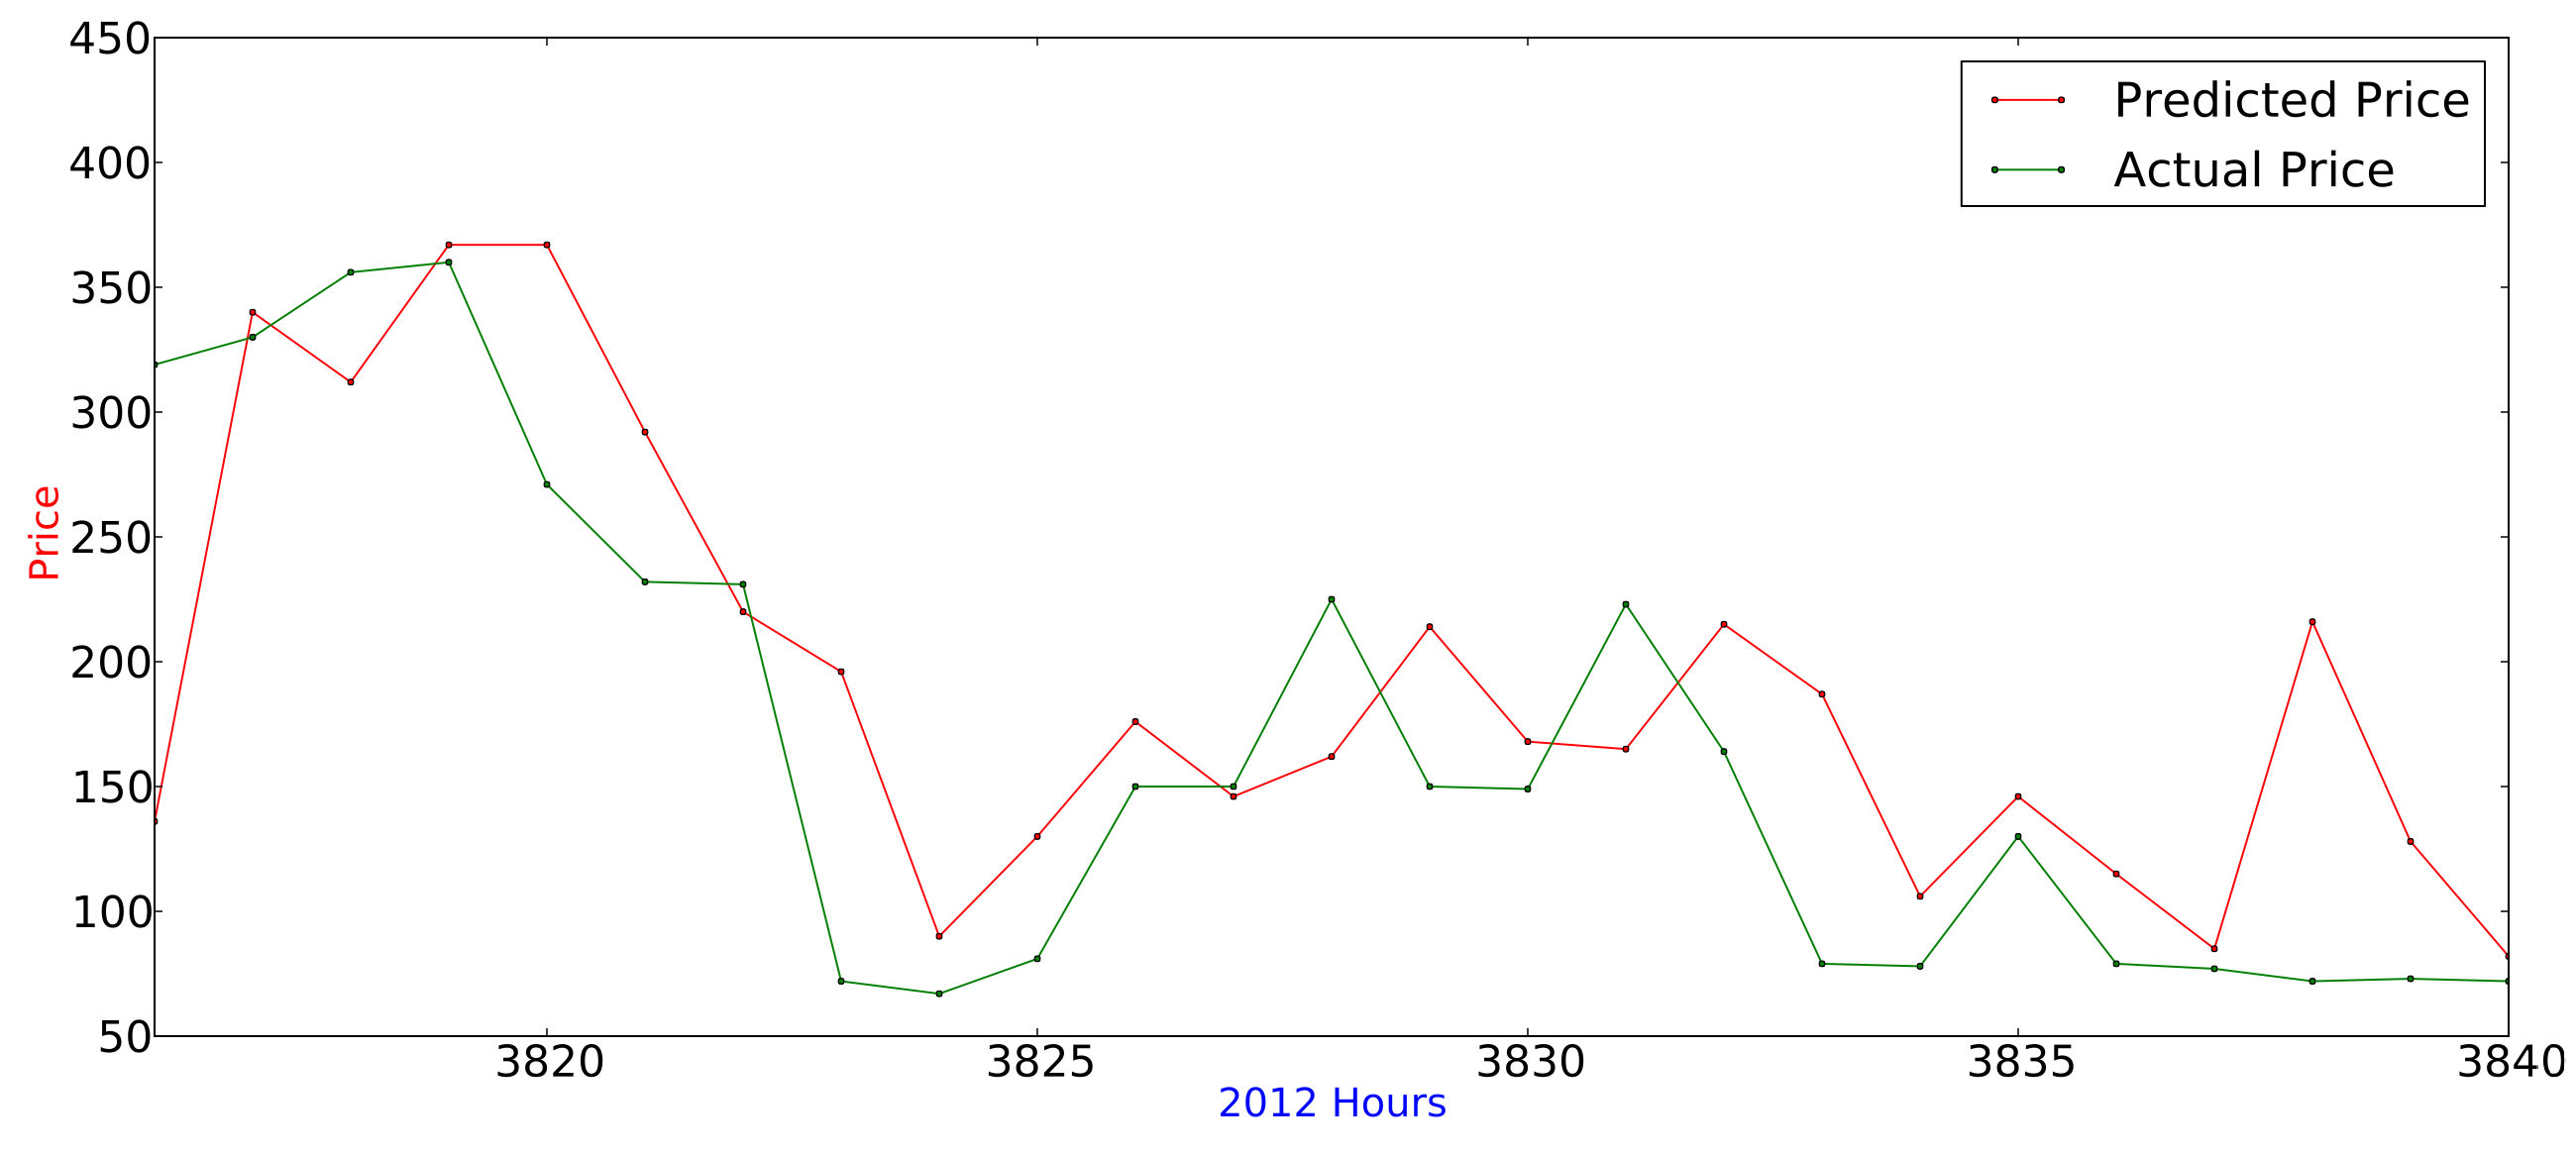
\includegraphics[width=\linewidth]{billeder/PriceExperimentalAnalysis/X2_X3_3816_3840_1hourAhead.png}
	\caption{1 Hour Ahead of \#1 forecast from experiment three. This is 24 hours from the middle of the year. (Skew, EWMA)}
	\label{fig:X2_X3_3816_3840_1hourahead}
\end{subfigure}
\caption{Activation functions}
\label{fig:1hourAhead}
\end{figure}

Variables: Price, Consumption, Wind Speed, Temperature, Time of Day (Matrix), Day of Week and Season of Year (Matrix)
\begin{table}[H]
\centering  % used for centering table
\resizebox{0.7\textwidth}{!}{
	\begin{tabular}{|c|c|c|c|c|c|c|} 
	\hline
	Rank & Curve & Skew & EWMA & Scatter & MAE & \% ranking\\ [0.5ex] % inserts table 
	\hline                  % inserts single horizontal line
	1  &       & \x    & \x    &       & 45,11 & - \\ \hline
	2  &       &       & \x    &       & 45,24 & 0,28\% \\ \hline
	3  & \x    & \x    & \x    &       & 45,43 & 0,7\% \\ \hline
	4  & \x    &       &       &       & 45,53 & 0,92\% \\ \hline
	5  & \x    & \x    &       & \x    & 46,45 & 2,98\% \\ \hline
	6  & \x    & \x    &       &       & 46,56 & 3,2\% \\ \hline
	7  &       &       & \x    & \x    & 46,76 & 3,65\% \\ \hline
	8  & \x    &       & \x    &       & 46,87 & 3,9\% \\ \hline
	9  &       & \x    & \x    & \x    & 47,25 & 4,73\% \\ \hline
	10 &       & \x    &       &       & 47,88 & 6,14\% \\ \hline
	11 &       &       &       & \x    & 47,88 & 6,14\% \\ \hline
	12 & \x    & \x    & \x    & \x    & 48,01 & 6,43\% \\ \hline
	13 & \x    &       & \x    & \x    & 48,13 & 6,68\% \\ \hline
	14 &       & \x    &       & \x    & 48,40 & 7,3\% \\ \hline
	15 & \x    &       &       & \x    & 49,68 & 10,12\% \\ \hline
	\end{tabular}
}
\caption{Calculated inputs effect on result \#2 from experiment 1.} % title of Table
\label{table:Statistical2} % is used to refer this table in the text
\end{table}

Variables: Price, Consumption, Wind Speed, Temperature, Time of Day (Matrix) and Month of Year (Matrix)
\begin{table}[H]
\centering  % used for centering table
\resizebox{0.7\textwidth}{!}{
	\begin{tabular}{|c|c|c|c|c|c|c|}
	\hline
	Rank & Curve & Skew & EWMA & Scatter & MAE & \% ranking\\ [0.5ex] % inserts table 
	\hline                  % inserts single horizontal line
	1  &       &       & \x    & \x    & 45,14 & - \\ \hline
	2  &       &       &       & \x    & 45,55 & 0,9\%  \\ \hline
	3  &       & \x    &       &       & 45,56 & 0,92\% \\ \hline
	4  &       & \x    &       & \x    & 45,60 & 1,02\% \\ \hline
	5  & \x    &       & \x    &       & 45,91 & 1,7\%  \\ \hline
	6  & \x    & \x    & \x    & \x    & 45,95 & 1,79\% \\ \hline
	7  & \x    & \x    &       &       & 45,99 & 1,89\% \\ \hline
	8  & \x    &       &       & \x    & 46,14 & 2,22\% \\ \hline
	9  & \x    &       &       &       & 46,58 & 3,18\% \\ \hline
	10 & \x    & \x    &       & \x    & 46,87 & 3,82\% \\ \hline
	11 &       &       & \x    &       & 46,98 & 4,08\% \\ \hline
	12 &       & \x    & \x    & \x    & 47,02 & 4,16\% \\ \hline
	13 & \x    & \x    & \x    &       & 47,08 & 4,3\%  \\ \hline
	14 & \x    &       & \x    & \x    & 47,94 & 6,2\%  \\ \hline
	15 &       & \x    & \x    &       & 47,98 & 6,29\% \\ \hline
	\end{tabular}
}
\caption{Calculated inputs effect on result \#3 from experiment 1.} % title of Table
\label{table:Statistical3} % is used to refer this table in the text
\end{table}

\subsubsection{Calculated inputs effect on a simple dataset}
To test the benefit of the calculated inputs on a vanilla dataset (that only contains the price and consumption) we conducted two more experiments - one with trimming(1\%) and one without trimming. We also did a simulation of the strategy described in paper \cite{singhal2011electricity} since this is where we got the selection of scatter prices from.

Test \#1 shown in table~\ref{table:price_consumption_x3} shows the calculated inputs applied on a dataset without trimming. The original test from experiment one can be seen in the price results appendix ~\ref{sec:priceResultAppendix} \#106 and gave us an MAE of 89. If we compare it to this test we see and improvement of 21.24\%. The most notable trend in the results in table~\ref{table:price_consumption_x3} is that nearly all of the scatter prices are the top results. That is also the case for the results in table~\ref{table:price_consumption_x3_1pTrim} (Same experiment with 1\% trim).

The most noteworthy are that the two are very similar and the one with trimming is actually worse when the EWMA strategy is applied. When we moved from experiment one to experiment two we saw that the ANN became more accurate when we trimmed away the largest spikes; this does not seem to be the case here. From this we can conclude that trimming has no effect on the dataset if all the other input variables are not included. In figure~\ref{fig:X3_Price_Consump_NoTrim} and ~\ref{fig:X3_Price_Consump_1pTrim} we see the similarities between the 1\% trim and the no-trim predictions. In figure ~\ref{fig:X3_Price_Consump_Worst} we see the same segment of the prediction as the other two but this one is with Curve, Skew, EWMA and 1\% trim. In the table ~\ref{table:price_consumption_x3} clearly see that it is way inferior. This is because the strategies applied accounts for to many of the inputs and it confuses more than it helps.

\begin{figure}[H]
\centering
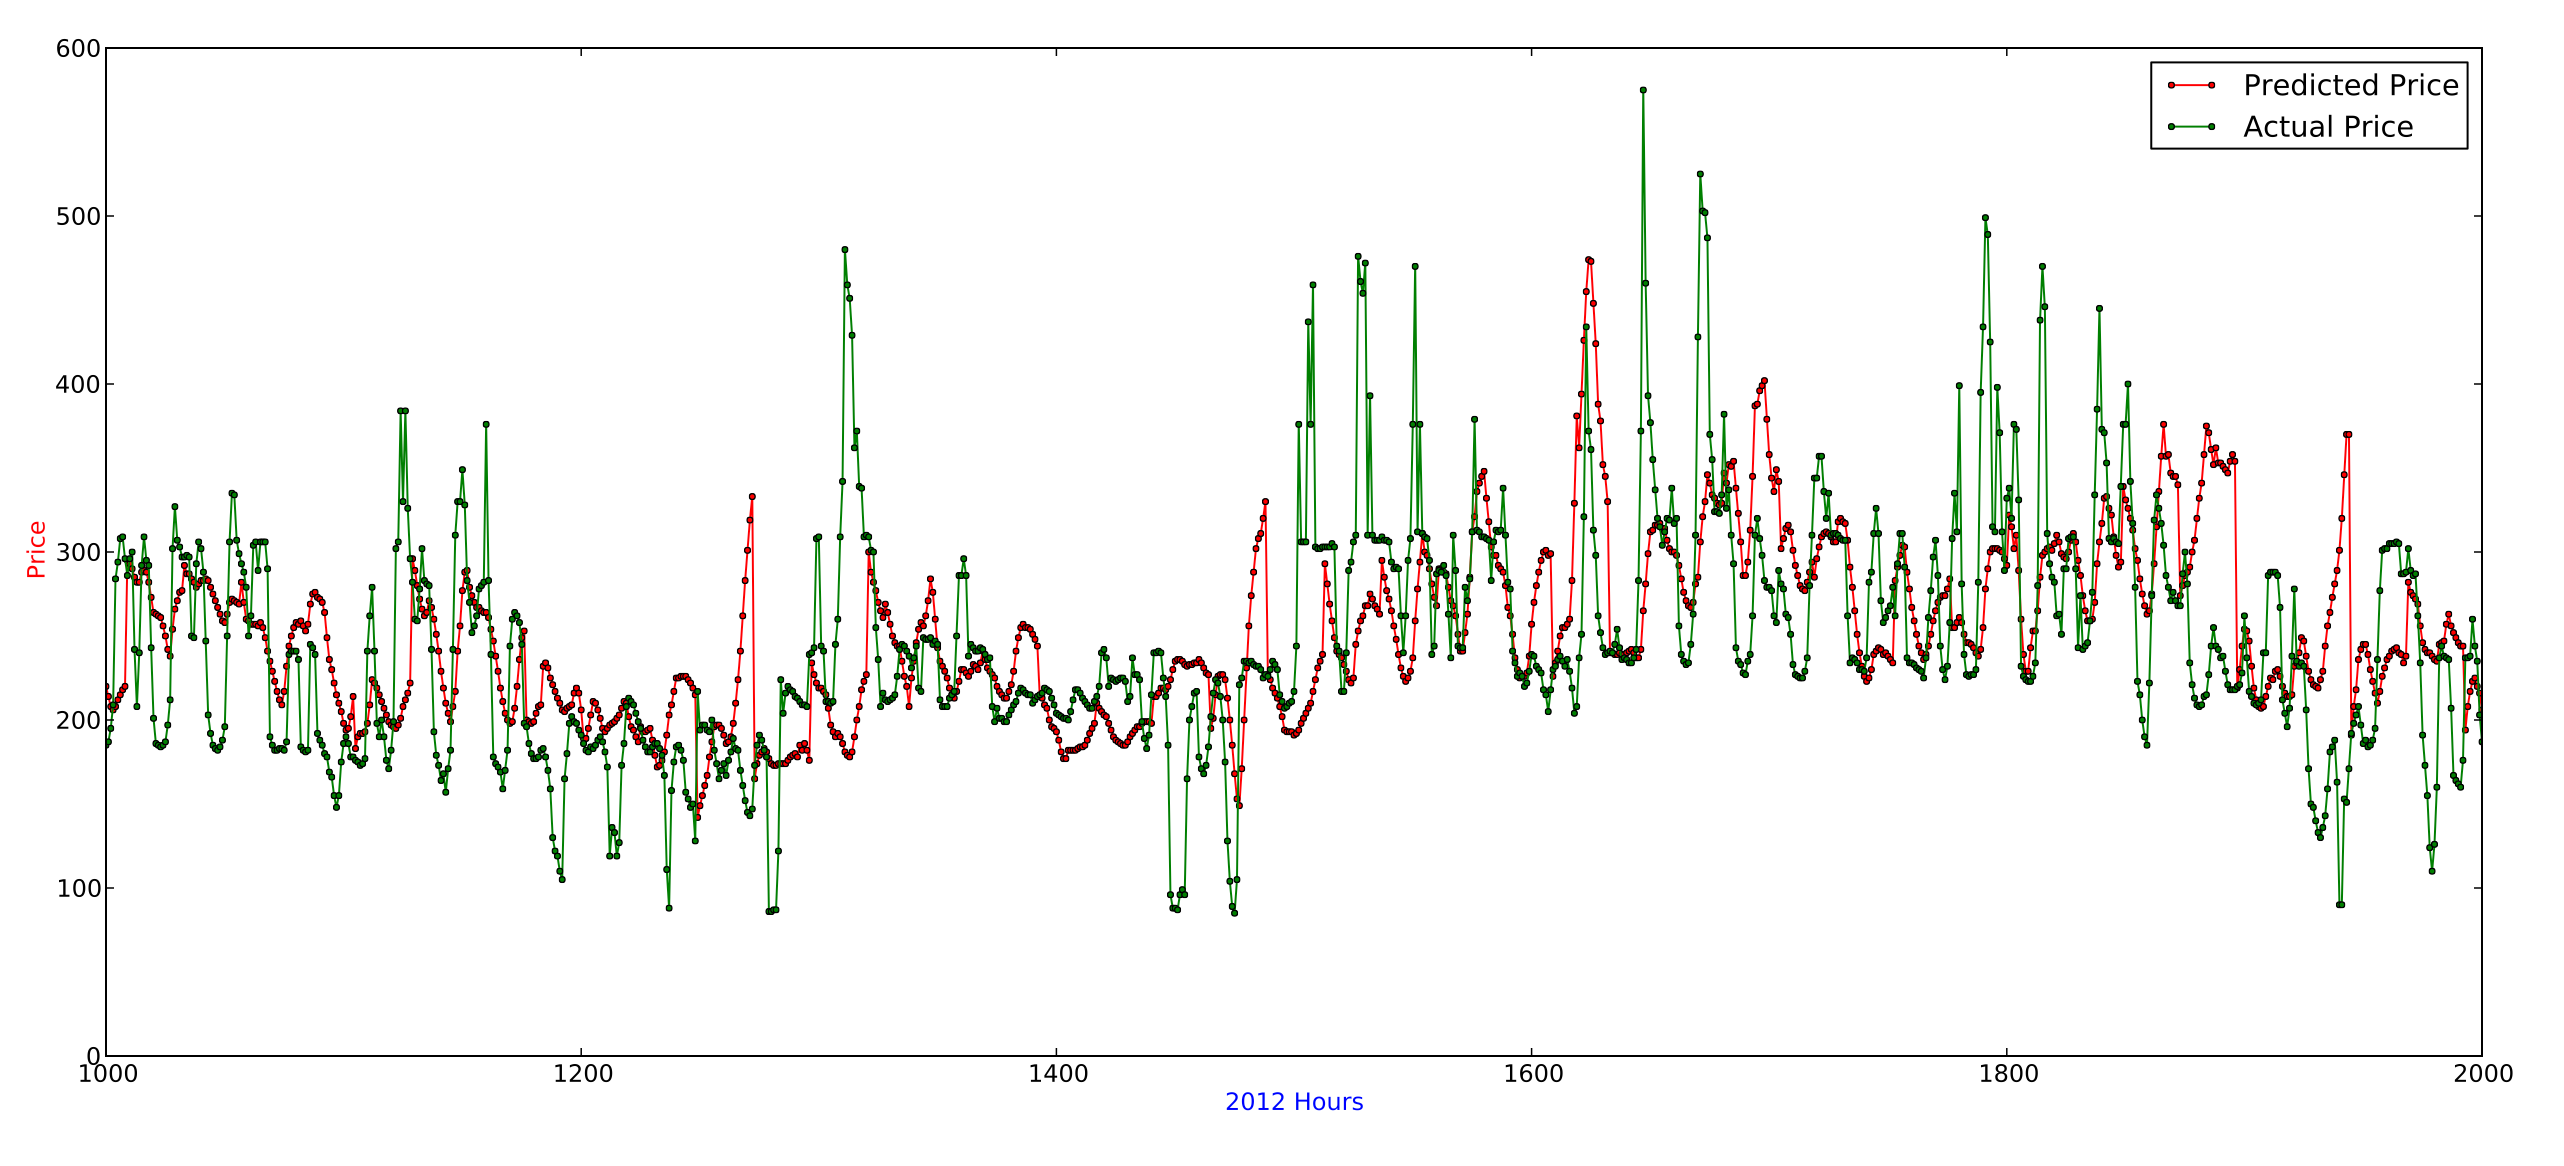
\includegraphics[width=\linewidth]{billeder/PriceExperimentalAnalysis/X3_Price_Consump_1pTrim.png}
\caption{Price and consumption with scatter and 1\% trim.)}
\label{fig:X3_Price_Consump_1pTrim}
\end{figure}

\begin{figure}[H]
\centering
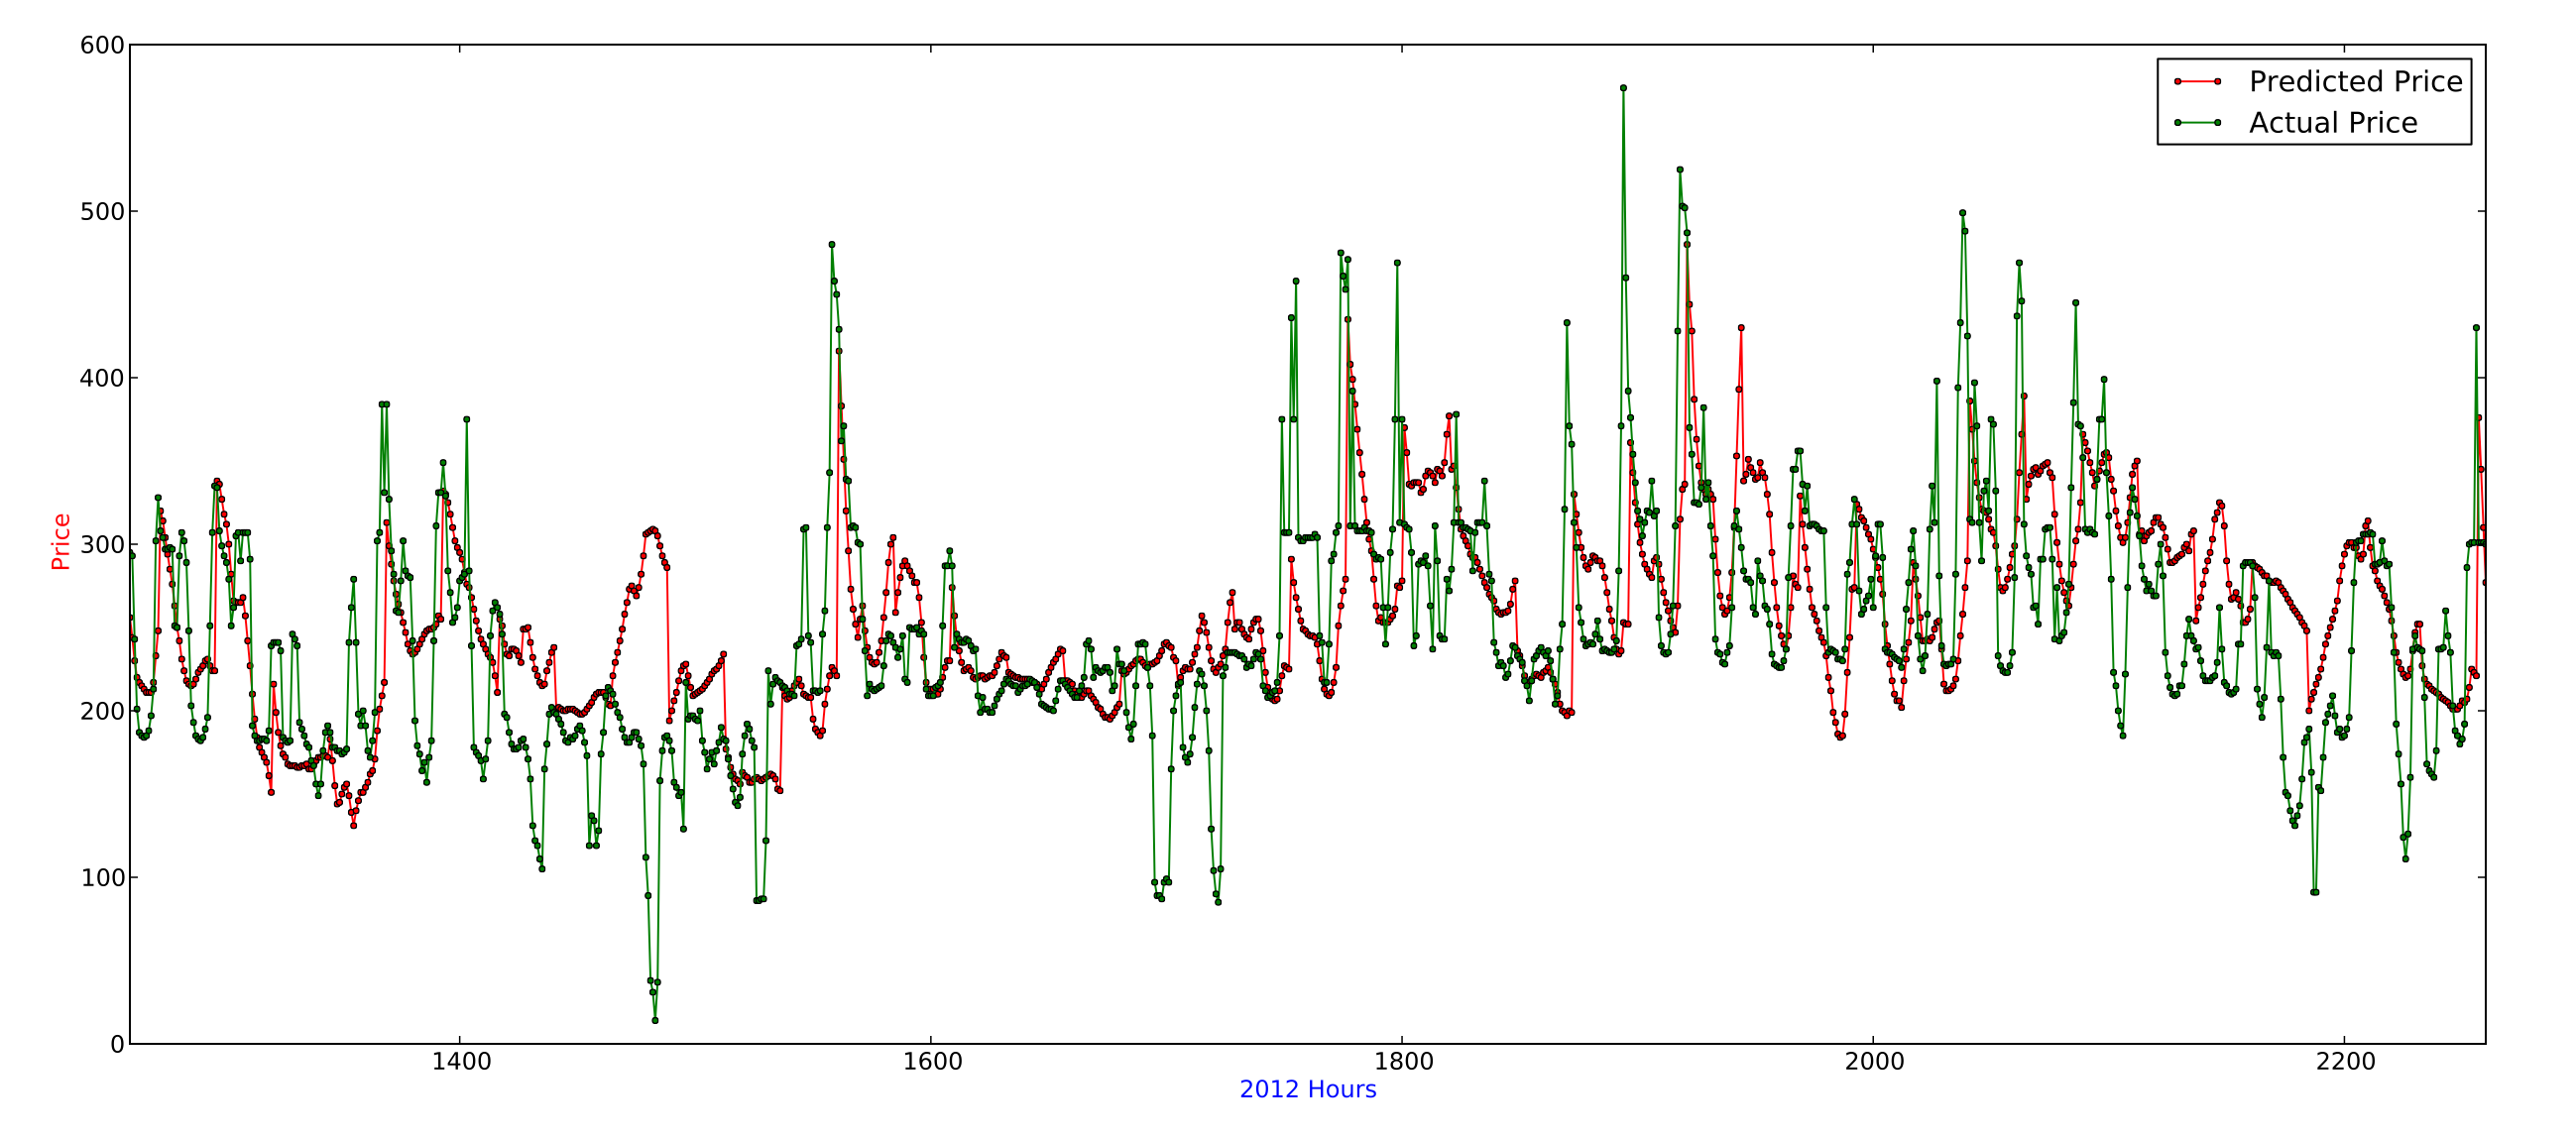
\includegraphics[width=\linewidth]{billeder/PriceExperimentalAnalysis/X3_Price_Consump_NoTrim.png}
\caption{Price and consumption with scatter and no trim.}
\label{fig:X3_Price_Consump_NoTrim}
\end{figure}

\begin{figure}[H]
\centering
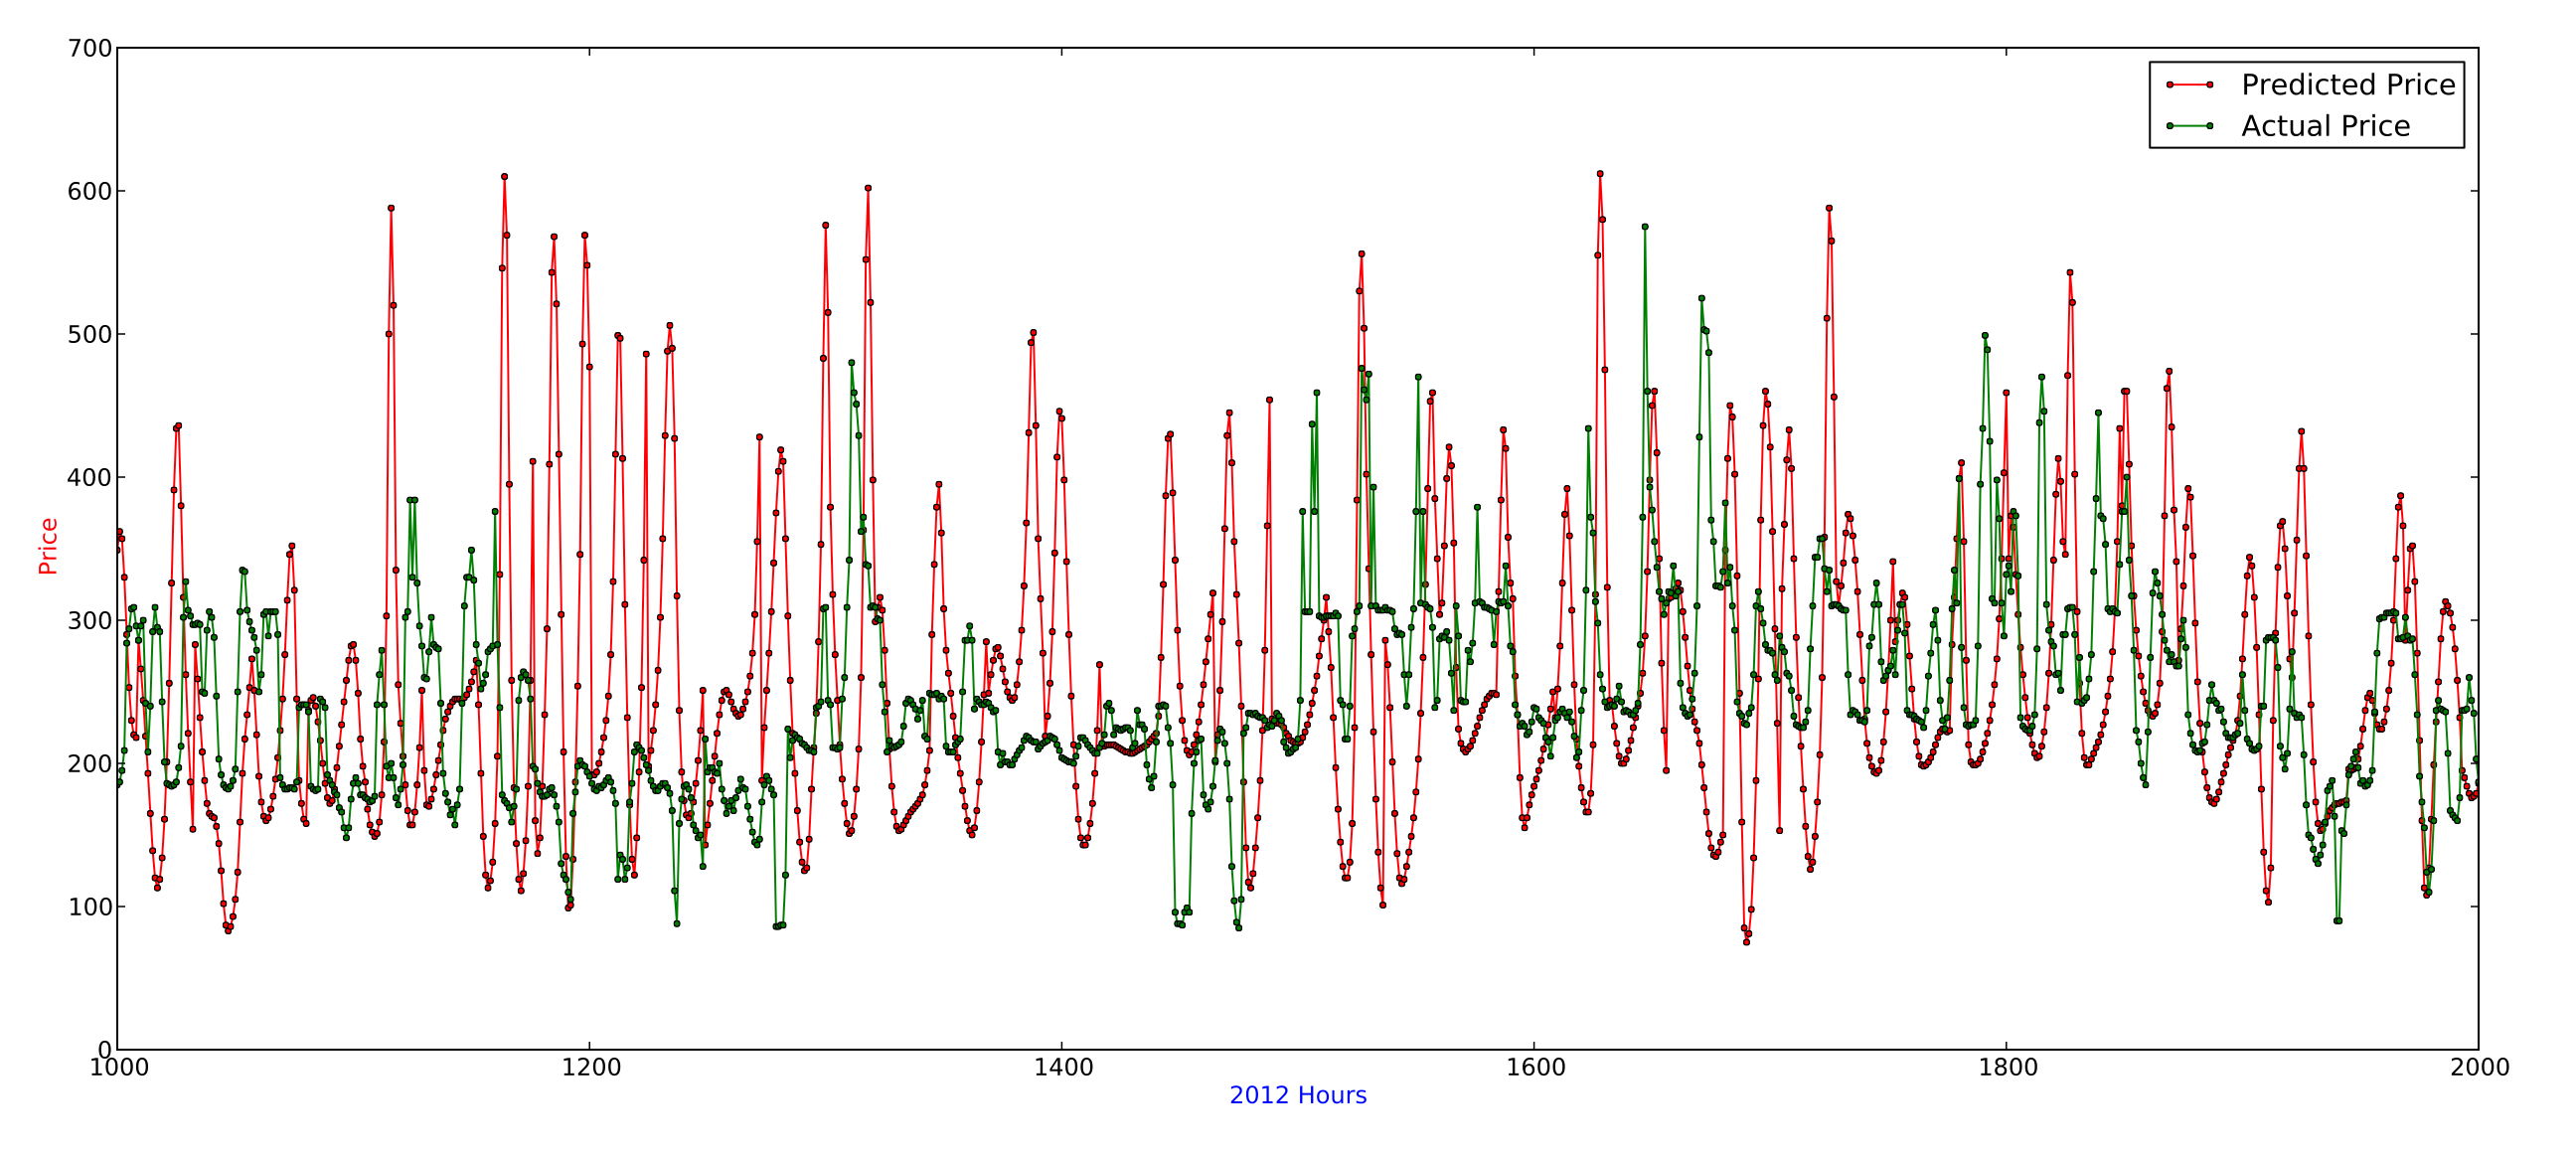
\includegraphics[width=\linewidth]{billeder/PriceExperimentalAnalysis/X3_Price_Consump_Worst.png}
\caption{Price and consumption with Curve, Skew, EWMA and 1\% trim.}
\label{fig:X3_Price_Consump_Worst}
\end{figure}

Variables: Price, Consumption and With no trimming
\begin{table}[H]
\centering  % used for centering table
\resizebox{0.7\textwidth}{!}{
	\begin{tabular}{|c|c|c|c|c|c|c|} % centered columns (7 columns)
	\hline
	Rank & Curve & Skew & EWMA & Scatter & MAE & \% ranking\\ [0.5ex] % inserts table 
	\hline                  % inserts single horizontal line
	1  &        &       &       & \x    & 73,43 & - \\ \hline
	2  &  \x    &       &       & \x    & 76,45 & 4,11\%  \\ \hline
	3  &        &       & \x    &       & 77,50 & 5,54\%  \\ \hline
	4  &  \x    &       & \x    & \x    & 77,54 & 5,6\%   \\ \hline
	5  &        & \x    &       & \x    & 79,17 & 7,82\%  \\ \hline
	6  &        &       & \x    & \x    & 80,67 & 9,86\%  \\ \hline
	7  &        & \x    & \x    & \x    & 80,85 & 10,11\% \\ \hline
	8  &  \x    & \x    & \x    & \x    & 81,97 & 11,63\% \\ \hline
	9  &        & \x    &       &       & 84,37 & 14,9\%  \\ \hline
	10 &  \x    & \x    &       & \x    & 84,86 & 15,57\% \\ \hline
	11 &  \x    & \x    & \x    &       & 86,49 & 17,79\% \\ \hline
	12 &  \x    &       & \x    &       & 86,95 & 18,41\% \\ \hline
	13 &        & \x    & \x    &       & 88,50 & 20,52\% \\ \hline
	14 &  \x    &       &       &       & 89,26 & 21,57\% \\ \hline
	15 &  \x    & \x    &       &       & 96,24 & 31,07\% \\ \hline
	\end{tabular}
}
\caption{calculated inputs on Price \& Consumption with no trim.} % title of Table
\label{table:price_consumption_x3} % is used to refer this table in the text
\end{table}

Variables: Price, Consumption and With 1\% trimming
\begin{table}[H]
\centering  % used for centering table
\resizebox{0.7\textwidth}{!}{
	\begin{tabular}{|c|c|c|c|c|c|c|} % centered columns (7 columns)
	\hline
	Rank & Curve & Skew & EWMA & Scatter & MAE & \% ranking\\ [0.5ex] % inserts table 
	\hline                  % inserts single horizontal line
	1  &        &       &       & \x    & 68,28  & - \\ \hline
	2  &  \x    & \x    &       & \x    & 69,40  & 1,63\%  \\ \hline
	3  &        & \x    &       & \x    & 70,17  & 2,77\%  \\ \hline
	4  &  \x    &       &       & \x    & 70,28  & 2,93\%  \\ \hline
	5  &        & \x    &       &       & 72,16  & 5,68\%  \\ \hline
	6  &  \x    & \x    &       &       & 75,31  & 10,29\% \\ \hline
	7  &  \x    &       &       &       & 77,14  & 12,97\% \\ \hline
	8  &  \x    &       & \x    & \x    & 93,86  & 37,46\% \\ \hline
	9  &  \x    & \x    & \x    & \x    & 94,21  & 37,98\% \\ \hline
	10 &        &       & \x    & \x    & 95,02  & 39,17\% \\ \hline
	11 &        & \x    & \x    & \x    & 97,79  & 43,22\% \\ \hline
	12 &        &       & \x    &       & 111,91 & 63,9\%  \\ \hline
	13 &        & \x    & \x    &       & 115,91 & 69,76\% \\ \hline
	14 &  \x    &       & \x    &       & 116,83 & 71,11\% \\ \hline
	15 &  \x    & \x    & \x    &       & 118,82 & 74,03\% \\ \hline
	\end{tabular}
}
\caption{calculated inputs on Price \& Consumption with 1\% trim.} % title of Table
\label{table:price_consumption_x3_1pTrim} % is used to refer this table in the text
\end{table}

\subsubsection{Clone experiment from literature}
The last iterations we did was a clone of the experiments conducted in~\cite{singhal2011electricity}. This setup includes price, consumption, time of day, day of week and scatter. We did the prediction both with 1\% and no trim as they did in the text (no spikes, small spikes and large spikes). The results can be seen in table ~\ref{table:scatter_text_no_trim} and ~\ref{table:scatter_text_1p_trim}. The results with trimming and the best strategies gives us a result of 52.04 MAE which is 14.75\% worse than the best result from table~\ref{table:Statistical1} and the results without trimming is 71.51 MAE which is 25.19\% worse than the best result from table~\ref{table:Top20Prices} in experiment one. We cannot compare the results directly to the ones they present in the paper because they only present a prediction of 48 hours and they do not tell us whether this is on unseen data or it is on the same dataset as they trained on. Neither do we know whether they simulate the full 48 hour prediction or they do it 1-hour at a time.

Variables: Price, Consumption, Time of Day, Day of Week and With no trimming
\begin{table}[H]
\centering  % used for centering table
\resizebox{0.7\textwidth}{!}{
	\begin{tabular}{|c|c|c|c|c|c|c|} % centered columns (7 columns)
	\hline
	Rank & Curve & Skew & EWMA & Scatter & MAE & \% ranking\\ [0.5ex] % inserts table 
	\hline                  % inserts single horizontal line
	1 &        & \x    &       & \x    & 71,51 & -       \\ \hline
	2 &        &       & \x    & \x    & 73,17 & 2,33\%  \\ \hline
	3 &        & \x    & \x    & \x    & 79,31 & 10,92\% \\ \hline
	4 &        &       &       & \x    & 80,20 & 12,16\% \\ \hline
	5 &  \x    & \x    & \x    & \x    & 82,03 & 14,73\% \\ \hline
	6 &  \x    &       & \x    & \x    & 89,82 & 25,61\% \\ \hline
	7 &  \x    &       &       & \x    & 94,26 & 31,83\% \\ \hline
	8 &  \x    & \x    &       & \x    & 94,90 & 32,72\% \\ \hline

	\end{tabular}
}
\caption{Scatter text~\cite{singhal2011electricity} with other calculated inputs and no trim} % title of Table
\label{table:scatter_text_no_trim} % is used to refer this table in the text
\end{table}

Variables: Price, Consumption, Time of Day, Day of Week and	With no trimming
\begin{table}[H]
\centering  % used for centering table
\resizebox{0.7\textwidth}{!}{
	\begin{tabular}{|c|c|c|c|c|c|c|} % centered columns (7 columns)
	\hline
	Rank & Curve & Skew & EWMA & Scatter & MAE & \% ranking\\ [0.5ex] % inserts table 
	\hline                  % inserts single horizontal line
	1 &  \x    & \x    &       & \x    & 52,04 & - \\ \hline
	2 &  \x    &       & \x    & \x    & 52,12 & 0,15\% \\ \hline
	3 &        & \x    & \x    & \x    & 53,22 & 2,27\% \\ \hline
	4 &        & \x    &       & \x    & 54,02 & 3,8\% \\ \hline
	5 &  \x    &       &       & \x    & 54,55 & 4,83\% \\ \hline
	6 &        &       & \x    & \x    & 55,80 & 7,23\% \\ \hline
	7 &        &       &       & \x    & 56,33 & 8,24\% \\ \hline
	8 &  \x    & \x    & \x    & \x    & 61,92 & 18,99\% \\ \hline

	\end{tabular}
}
\caption{Scatter text~\cite{singhal2011electricity} with other calculated inputs and 1\% trim} % title of Table
\label{table:scatter_text_1p_trim} % is used to refer this table in the text
\end{table}

\subsubsection{Conclusion}
The calculated inputs that we applied in this experiment did help the curve analysis but only slightly. The best improvement gave a result that was 4.10\% better than the same combination in experiment 2. The results also show that the calculated inputs will at worst just be the same as before. So if we apply them and they do not work then the result and MAE will not suffer from this.

The results from the simple dataset (last known price and consumption) showed us that if we apply calculated inputs to this dataset it will improve quite a bit. The improvement makes it as good as the best combination from experiment one. The downside with this is that we are not able to improve it further. So it gets stuck with that error margin. We conducted the same trial with a 1 \% trimmed dataset and here we saw no improvement. It shows that our calculated inputs actually can improve some datasets but it does not improve our best combination.

The last part was a comparison with the paper~\cite{singhal2011electricity} where they have a setup which we copied in this experiment. Their setup did a good job of predicting the price but our setup gave a better result. We cannot compare the results directly due to a lack of information on how they conducted their trials. We did try on both a dataset with and without trimming applied. In this case the trimmed dataset gave a better result.

\newpage
\subsection{Experiment four: Black box optimization}
\label{sec:priceExperimentFour}
We here show the impacts of epochs used to train the network and the size of the training dataset. We also show how the time dimension of doing these tests are affected by these parameters. Black box optimization also covers the number of hidden layers and the neuron count in these. We chose not to do these experiments since we used a pruning algorithm to find the most optimal combination of neurons and layers for each input combination as described in section~\ref{sec:testProcedure} and in section~\ref{sec:pruning}.

\subsubsection{Variables}
All of these tests were conducted using the best combination seen in table ~\ref{table:Statistical1}. Giving us the following combination:
\begin{itemize}
	\item Price
	\item Consumption
	\item Wind Speed
	\item Temperature
	\item Time of Day (Matrix)
	\item Day of Week (Matrix)
	\item Season of Year (Matrix)
	\item Skewness
	\item EWMA
\end{itemize}

The following parameters were tested:

\begin{itemize}
	\item Epochs from 1 to 3000
	\item Dataset sizes equivalent to 1/4, 1/2, 3/4 and a 1/1 year
\end{itemize}

\subsubsection{Hypothesis}
We expect the results from these tests to show that the time used to make a years prediction will increase with the numbers of epochs and it will increase with the size of the dataset. We expect the best epochs to be in the lower end of the scale presented above. The best results from the dataset test is expected to be 1/4 year or 1/2 year sizes. These assumptions are based on what we described in the Forecasting Model chapter~\ref{ch:forecastingModel}.

\todo{Soerg for at det giver mening i forhold til hvad vi har skrevet i det kapitel.}

\subsubsection{Results}
The results from table~\ref{table:Dataset_size} shows the impact of increasing the size of the training dataset. The influence of increasing the size shows a deviation of 7,19\%. It shows that the best result are the size equivalent to half a year. The second best are the 1 year prediction which might be because we included the seasonal parameters as we showed in experiment one; where the addition of the Month of Year(MoY) parameter increased the performance of a one year training set. The one we have used throughout the preceding results are the third best and gave a result that was 6,46\% worse than the best thus we might be able to increase some of the scores from earlier experiments if we use a dataset consisting of data from half a year. Another interesting point here is how the time to a prediction increases linearly with the amount of entries in the dataset - from 232 seconds(3.9 minutes) to 844 seconds(14.1 minutes). The increase in time are worth mentioning since we are doing hourly based calculations. If a fast prediction is needed a trader might chose a faster method with a loss in performance.

\todo{Write something about under- and overtraining. Does not seem to be the case here.}

\begin{table}[H]
\centering  % used for centering table
\resizebox{0.8\textwidth}{!}{
	\begin{tabular}{|c|c|c|c|c|c|} % centered columns (7 columns)
	\hline
	Entries & Time(seconds) & H1 & H2 & MAE & \% ranking\\ [0.5ex] % inserts table 
	\hline                  % inserts single horizontal line
	4378 & 397,28 & 6  & 11 & 46,34 & - \\ \hline
	8756 & 844,68 & 12 & 5  & 47,82 & 3,19\% \\ \hline
	2189 & 232,87 & 6  & 18 & 49,33 & 6,46\% \\ \hline
	6567 & 677,33 & 14 & 6  & 49,67 & 7,19\% \\ \hline
	\end{tabular}
}
\caption{The results from the dataset size test.} % title of Table
\label{table:Dataset_size} % is used to refer this table in the text
\end{table}

In table~\ref{table:Epochs} we see the effects of epochs used when training the network. We see a tendency that values between 100 and 1000 are the best number of epochs to use in this network. 40 epochs also perform very well which are a bit surprising since the number of epochs used to train the network reflects how many iterations the network undergoes to find the best match between the weights. The under fitting of the weights can be seen in 1 epoch training(\#27 in ~\ref{table:Epochs}) where the network gets one attempt to correct the weights and find a generalization of the parameters (which would be a lucky guess if that happened). The 1 epoch run can be seen in figure~\ref{fig:1epoch}. We also see over fitting of the dataset when running more than 1800 epochs the performance drops at least 10.26\% and gets worse with more epochs. Another thing to notice here are the time used to run the pruning algorithm and predict the next years data. We can see how the time rises when the number of epochs rises. Also the number of neurons in each layer have an influence on the time used to do the predictions (more neurons equals more time used).

\todo{Time perspective not that relevant when we are talking 24 hours ahead because we are not predicting a full year every time we run it thus making the difference in time very insignificant.}

\begin{figure}[H]
\centering
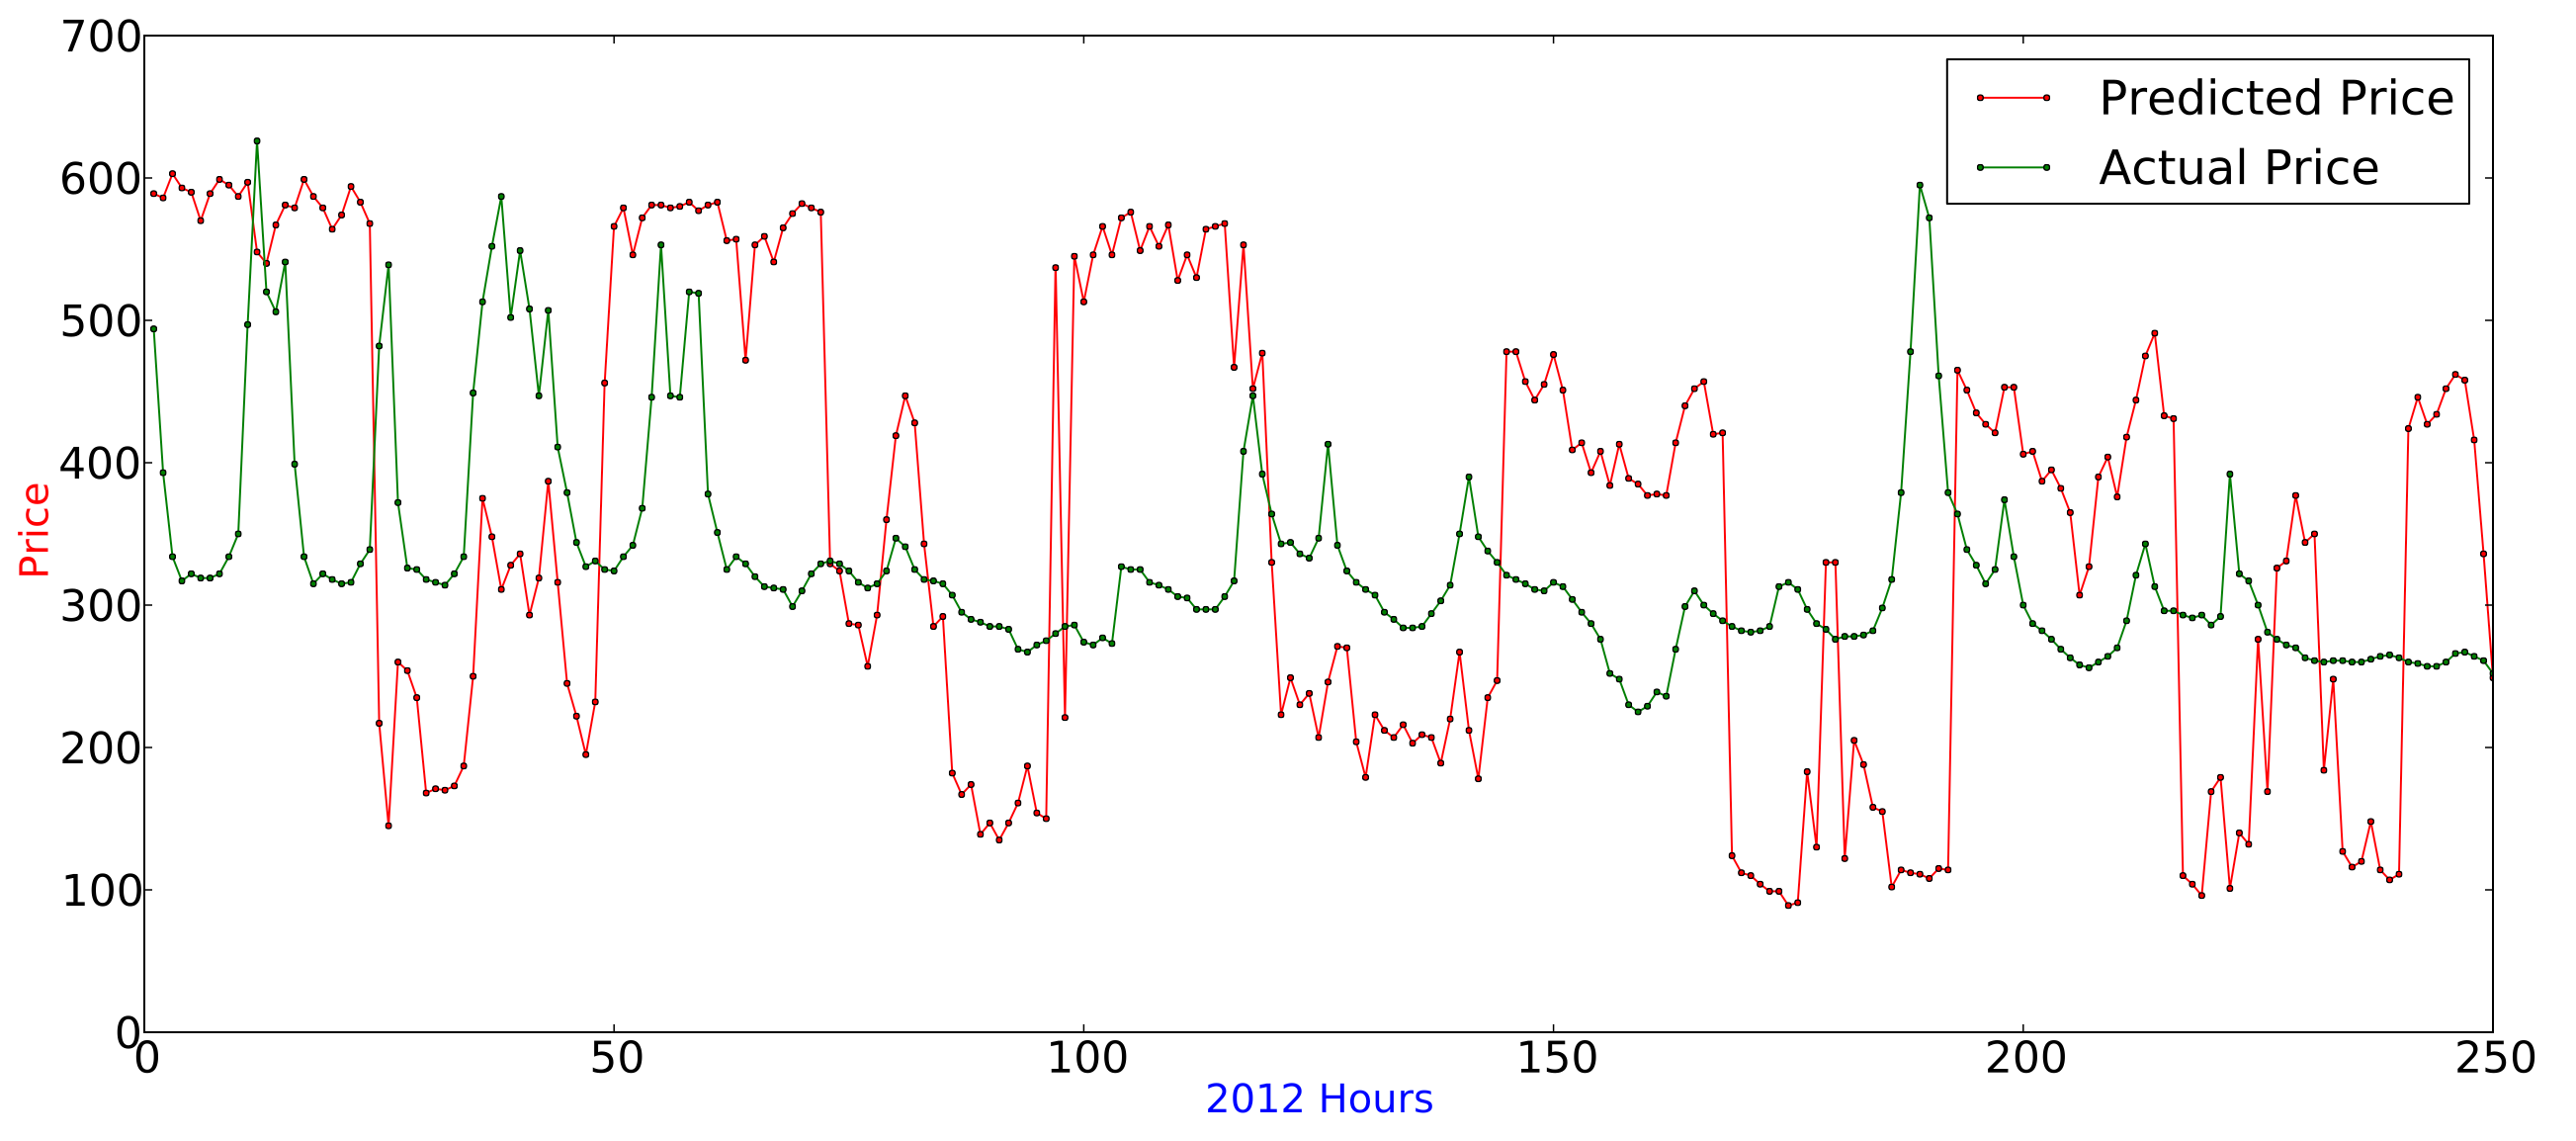
\includegraphics[width=\linewidth]{billeder/PriceExperimentalAnalysis/1EpochTraining.png}
\caption{Shows how the predictions are done when the network is trained for 1 epoch before every prediction}
\label{fig:1epoch}
\end{figure}

\begin{table}[H]
\centering  % used for centering table
\resizebox{0.8\textwidth}{!}{
	\begin{tabular}{|c|c|c|c|c|c|c|} % centered columns (7 columns)		
	\hline
	\# & Epochs & Time(seconds) & H1 & H2 & MAE & \% ranking \\ [0.5ex] % inserts table 
	\hline                  % inserts single horizontal line
	1  & 500  &450.19  & 12 & 11 & 45.17 & - \\ \hline
	2  & 600  &375.02  & 7  & 11 & 46.14 & 2.16\% \\ \hline
	3  & 900  &415.28  & 8  & 3  & 47.32 & 4.77\% \\ \hline
	4  & 1100 &566.83  & 10 & 5  & 47.40 & 4.95\% \\ \hline
	5  & 200  &264.03  & 14 & 8  & 47.92 & 6.09\% \\ \hline
	6  & 100  &213.95  & 14 & 11 & 48.13 & 6.55\% \\ \hline
	7  & 1600 &807.21  & 6  & 17 & 48.23 & 6.78\% \\ \hline
	8  & 300  &315.01  & 14 & 10 & 48.41 & 7.17\% \\ \hline
	9  & 1200 &676.83  & 10 & 9  & 48.74 & 7.91\% \\ \hline
	10 & 40   &185.18  & 17 & 8  & 49.34 & 9.24\% \\ \hline
	11 & 400  &345.01  & 12 & 8  & 49.37 & 9.3\% \\ \hline
	12 & 1800 &1496.67 & 5  & 1  & 49.80 & 10.26\% \\ \hline
	13 & 800  &518.7   & 8  & 16 & 50.15 & 11.02\% \\ \hline
	14 & 1000 &612.22  & 8  & 18 & 50.67 & 12.19\% \\ \hline
	15 & 1300 &877.29  & 13 & 13 & 50.78 & 12.42\% \\ \hline
	16 & 1500 &691.92  & 7  & 8  & 50.82 & 12.52\% \\ \hline
	17 & 2400 &2510.23 & 6  & 11 & 51.58 & 14.2\% \\ \hline
	18 & 2200 &3296.05 & 10 & 25 & 51.72 & 14.5\% \\ \hline
	19 & 3000 &3600.85 & 7  & 19 & 52.09 & 15.33\% \\ \hline
	20 & 700  &471.98  & 7  & 20 & 52.26 & 15.7\% \\ \hline
	21 & 2000 &3035.47 & 13 & 16 & 53.56 & 18.57\% \\ \hline
	22 & 20   &175.38  & 19 & 8  & 53.69 & 18.87\% \\ \hline
	23 & 1400 &978.75  & 12 & 18 & 54.41 & 20.46\% \\ \hline
	24 & 2800 &3202.93 & 7  & 15 & 55.20 & 22.2\% \\ \hline
	25 & 2600 &3286.09 & 11 & 9  & 57.69 & 27.73\% \\ \hline
	26 & 10   &177.02  & 14 & 6  & 58.75 & 30.07\% \\ \hline
	27 & 1    &168.82  & 15 & 10 & 122.50 & 171.2\% \\ \hline
	\end{tabular}
}
\caption{The results from the epochs experiment.} % title of Table
\label{table:Epochs} % is used to refer this table in the text
\end{table}

\subsubsection{Conclusion}
From this experiment we see that the optimal (for this input combination) training dataset size is half a year of data. We see an improvement of 6,46\% compared to the dataset size we have used in the prior experiments thus a better result from those experiments are expected if we use half a year of data instead of just a quarter of a year. The time consumed with this increase in the dataset would have doubled the time we used to conduct the trials. The time used to predict a full year are very close to a 1-to-1 correlation with the size of the dataset.

The epochs used to train the network shows that values in the hundreds (100-900) dominate the top 10 results in~\ref{table:Epochs}. The best result is 500 epochs and shows an improvement over 200 epochs of 6.09\% which we used in prior experiments. These results also show how the time increases when the number of epochs increases. This increase is not as apparent as it is in the dataset size experiments - this is because of the different neuron counts in the hidden layers which also influences the time it takes to conduct one experimental iteration. We still see a tendency where higher number of epochs results in more time consumed doing the experiment.

\newpage
\subsection{Experiment five: Step-ahead forecasting}
\label{sec:priceExperimentFive}
Here we did a test of how the predictions behave when we increase the hours to use in step-ahead predictions. We did a 1-hour ahead prediction and kept increasing the number until we hit 24 hours. We also conducted a test to see what the effects of shifting the starting offset are.

\subsubsection{Variables}
This test were conducted using the best combination seen in table ~\ref{table:Statistical1}. Giving us the following combination:
\begin{itemize}
	\item Price
	\item Consumption
	\item Wind Speed
	\item Temperature
	\item Time of Day (Matrix)
	\item Day of Week (Matrix)
	\item Season of Year (Matrix)
	\item Skewness
	\item EWMA
\end{itemize}

The following parameters were tested:

\begin{itemize}
	\item Hours to use in step-ahead forecasting.
\end{itemize}

\subsubsection{Hypothesis}
In this experiment we anticipate to see a decrease in MAE as we increase the number of hours the ANN has to predict. The reason for this is the elevation of the error when we add more hours to predict ahead. The elevation comes from the last known price which will be the last predicted price from hour 2 and onwards thus elevating the error. The prediction of price relies in a great extend on the last-known price and therefore it will have a significant effect on the price.

We also expect to see that the MAE will change when we shift the offsets. The offsets decide where the first and (in most cases) best prediction will start. If these first predictions hit good spots where the error margin will not rise as fast as other spots around it, then we will see a lower MAE.

\subsubsection{Results}
In table~\ref{table:XHoursAhead} we see the results from this experiment. The MAE is linear with the number of hours ahead during the first 10 predictions. From there it gets a bit more random which gives the worst result but 22, 23 and 24 again follows a linear pattern. From around 10 hours ahead the increase in MAE seems to be slowing down. This is because it is not only the last known price that dictates what the new prediction will be. The other input parameters (wind speed, time of day etc.) will also influence the price. So when we hit a certain point in the prediction (which seems to be around 10 predictions ahead) the other input parameters will prevent the elevation of errors further. This can be seen in figure~\ref{fig:24HoursAhead_elevationOfError} where the black lines denotes 24 hours. We see in the 24 hours prediction (with the black box overlay) how the error is rising but when the prices start to fall so does the prediction. If it had been the last known price that dictated the next prediction then the predictions would have kept rising and so would the MAE. This is why we see that the MAE stagnates at about 10 hours ahead and above.

\begin{figure}[H]
\centering
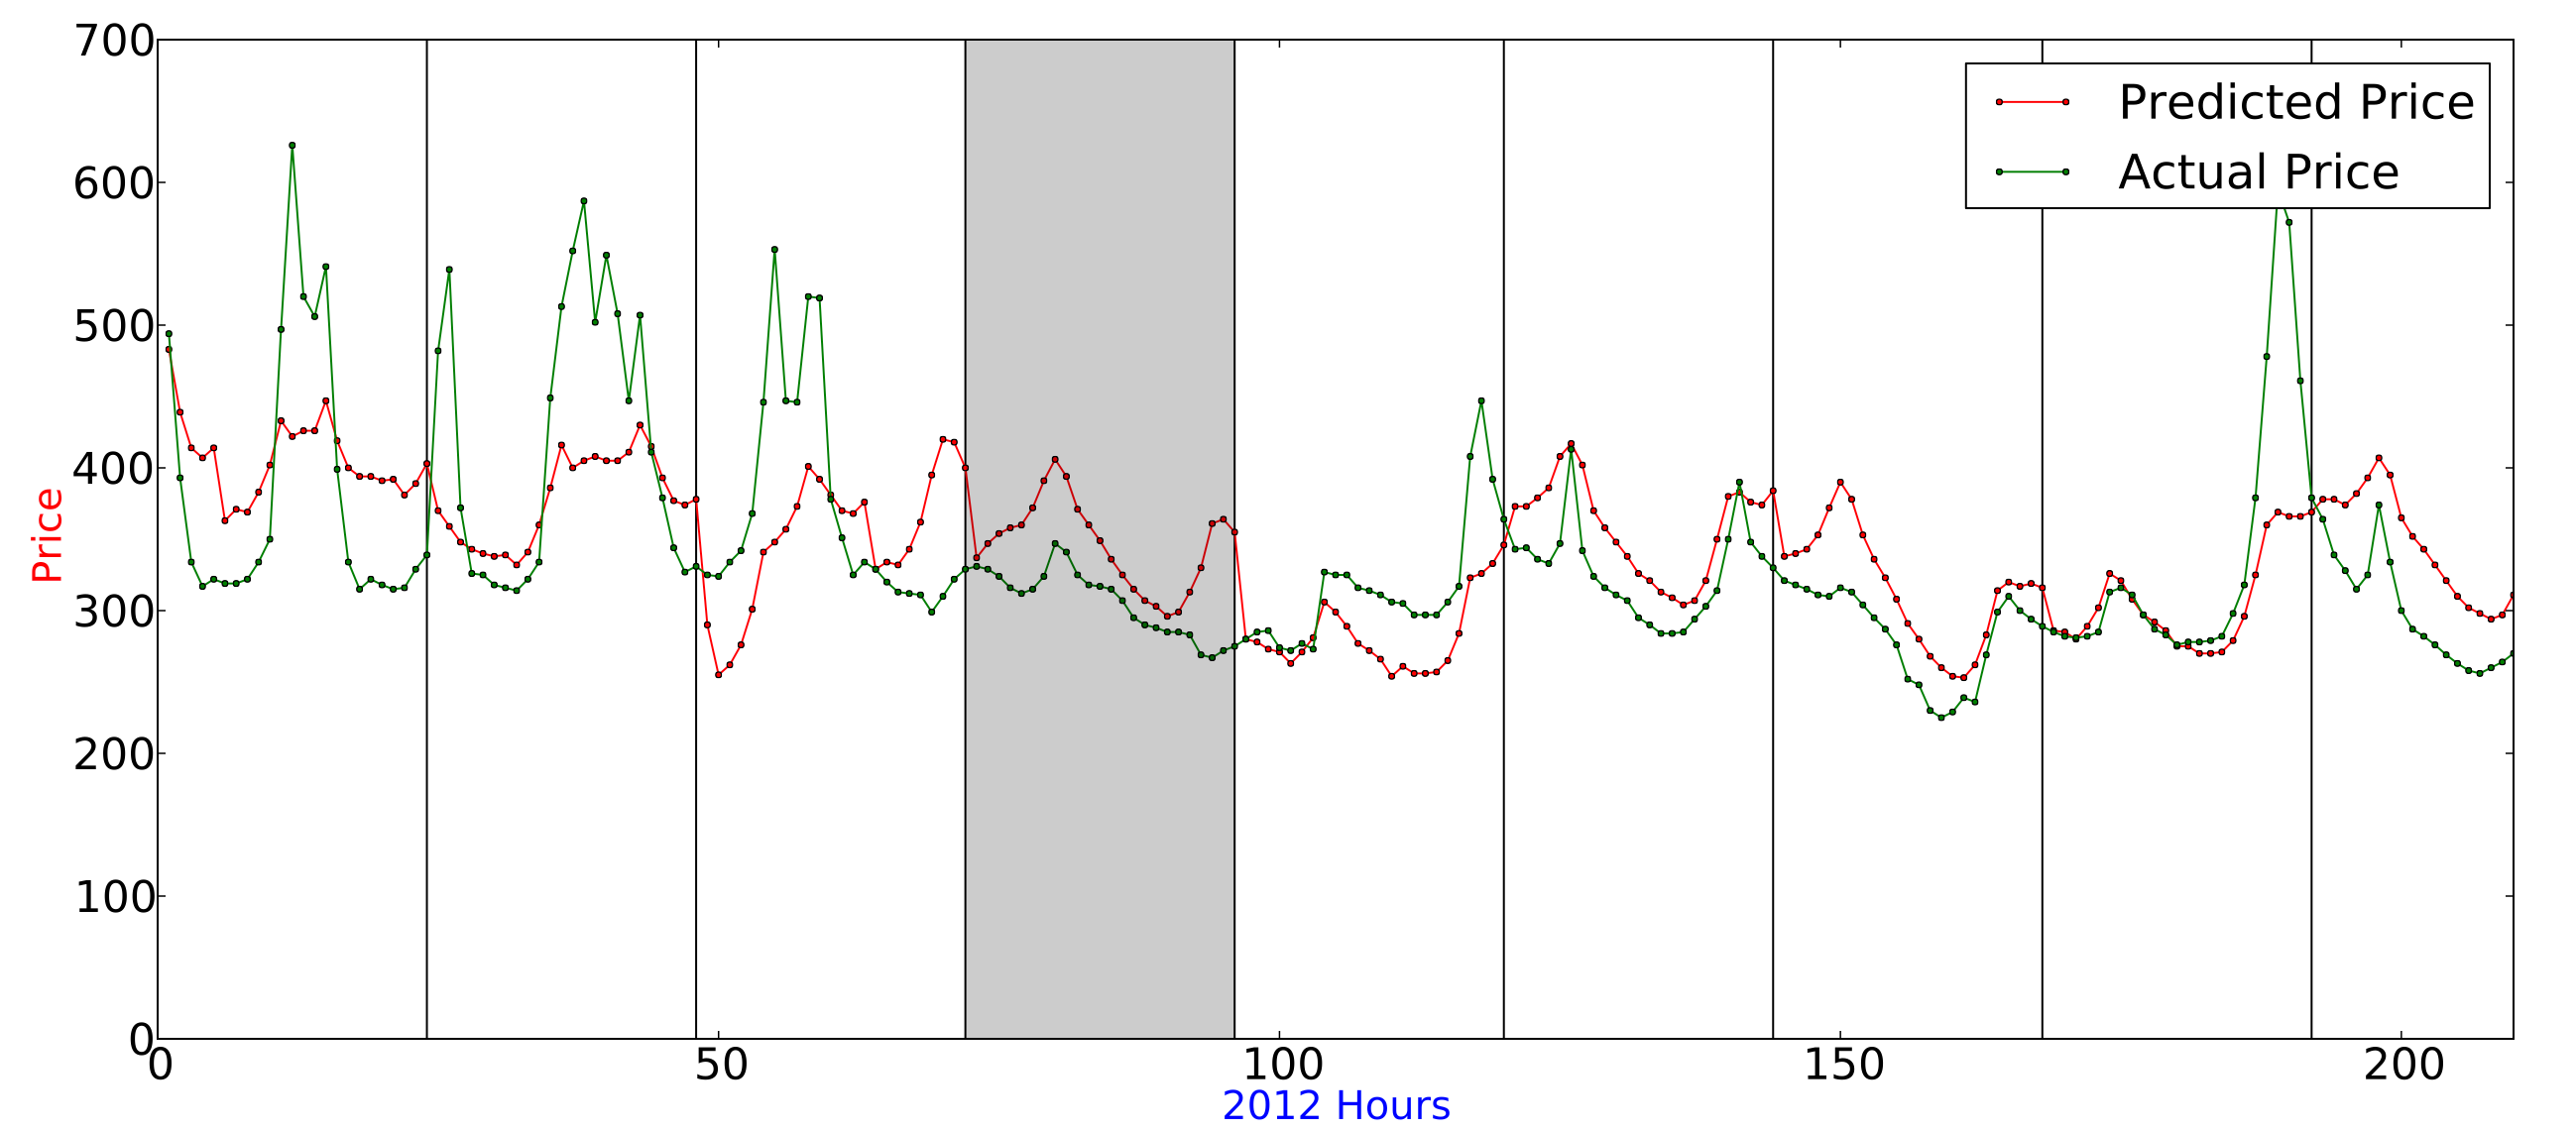
\includegraphics[width=\linewidth]{billeder/PriceExperimentalAnalysis/24HoursAhead_ElevationOfErrorExample.png}
\caption{Prediction of 24 hours ahead.}
\label{fig:24HoursAhead_elevationOfError}
\end{figure}

In the 2 hours ahead prediction seen in figure~\ref{fig:2HoursAhead} we see how well the predictions are when we only predict 2 hours ahead. This is due to the limitation of the elevation of error which happens when we only have 1 hour dependent on an earlier prediction.

\begin{figure}[H]
\centering
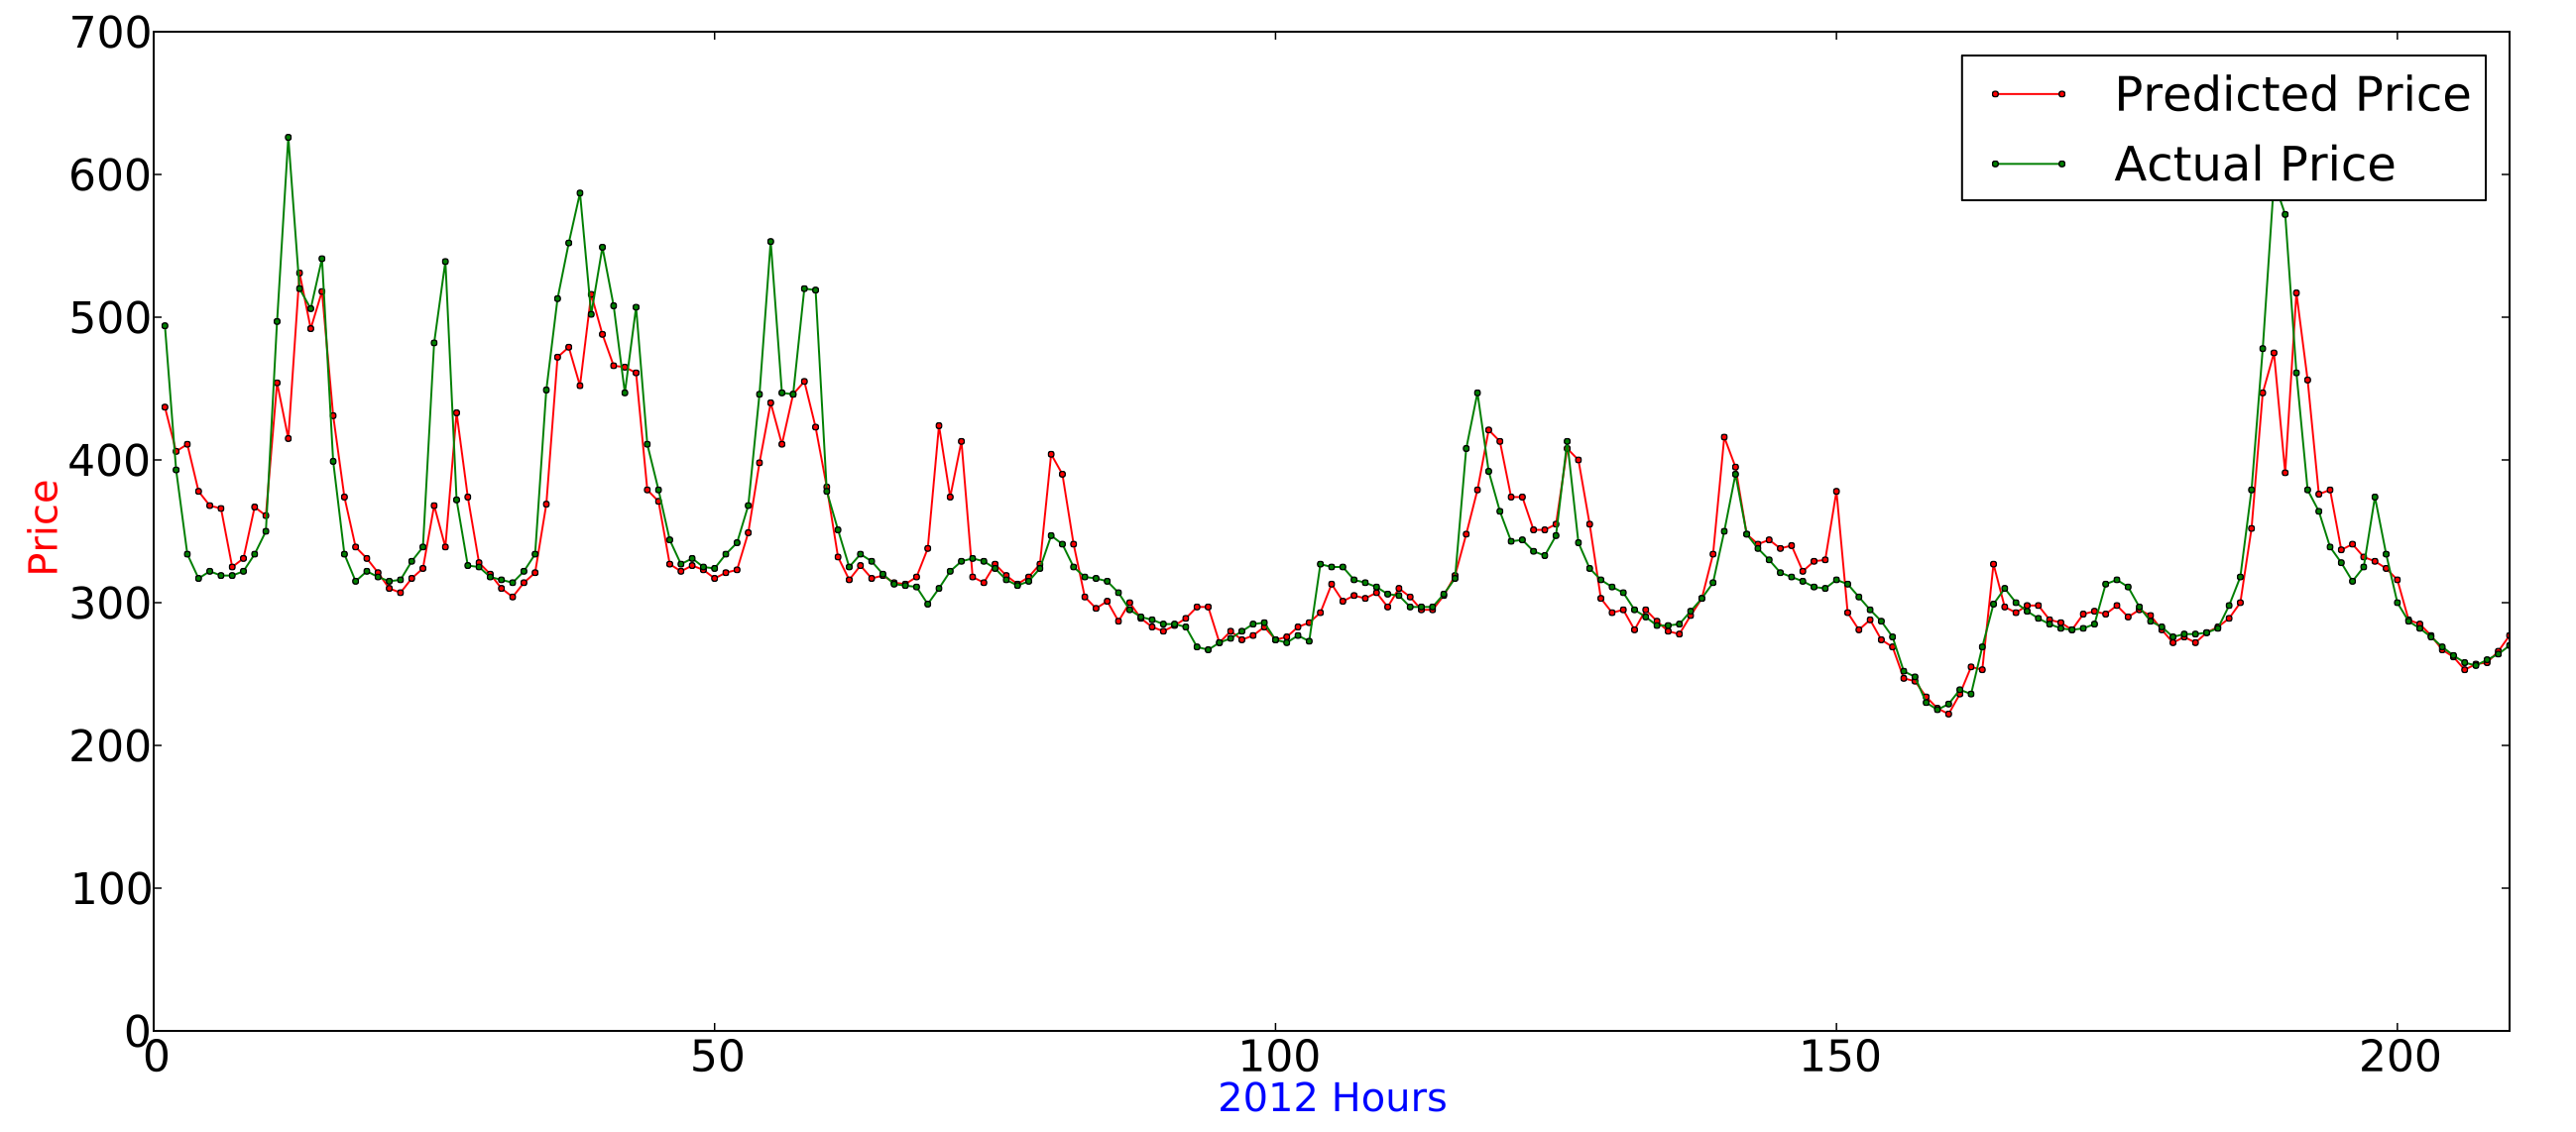
\includegraphics[width=\linewidth]{billeder/PriceExperimentalAnalysis/2HoursAheadForecast.png}
\caption{Prediction of 2 hours ahead}
\label{fig:2HoursAhead}
\end{figure}

In the 10 hours ahead predict seen in figure~\ref{fig:10HoursAhead} we again see how the elevation happens. The black lines in the figure shows when we shift from one prediction cycle of 10 hours to the next. It is very clear in the figure how the predictions are corrected to fit the curve better every time we reset the prediction. From the beginning of every prediction cycle the next result will be based on correct data thus not relying on a potentially faulty prediction done earlier in the cycle.

\begin{figure}[H]
\centering
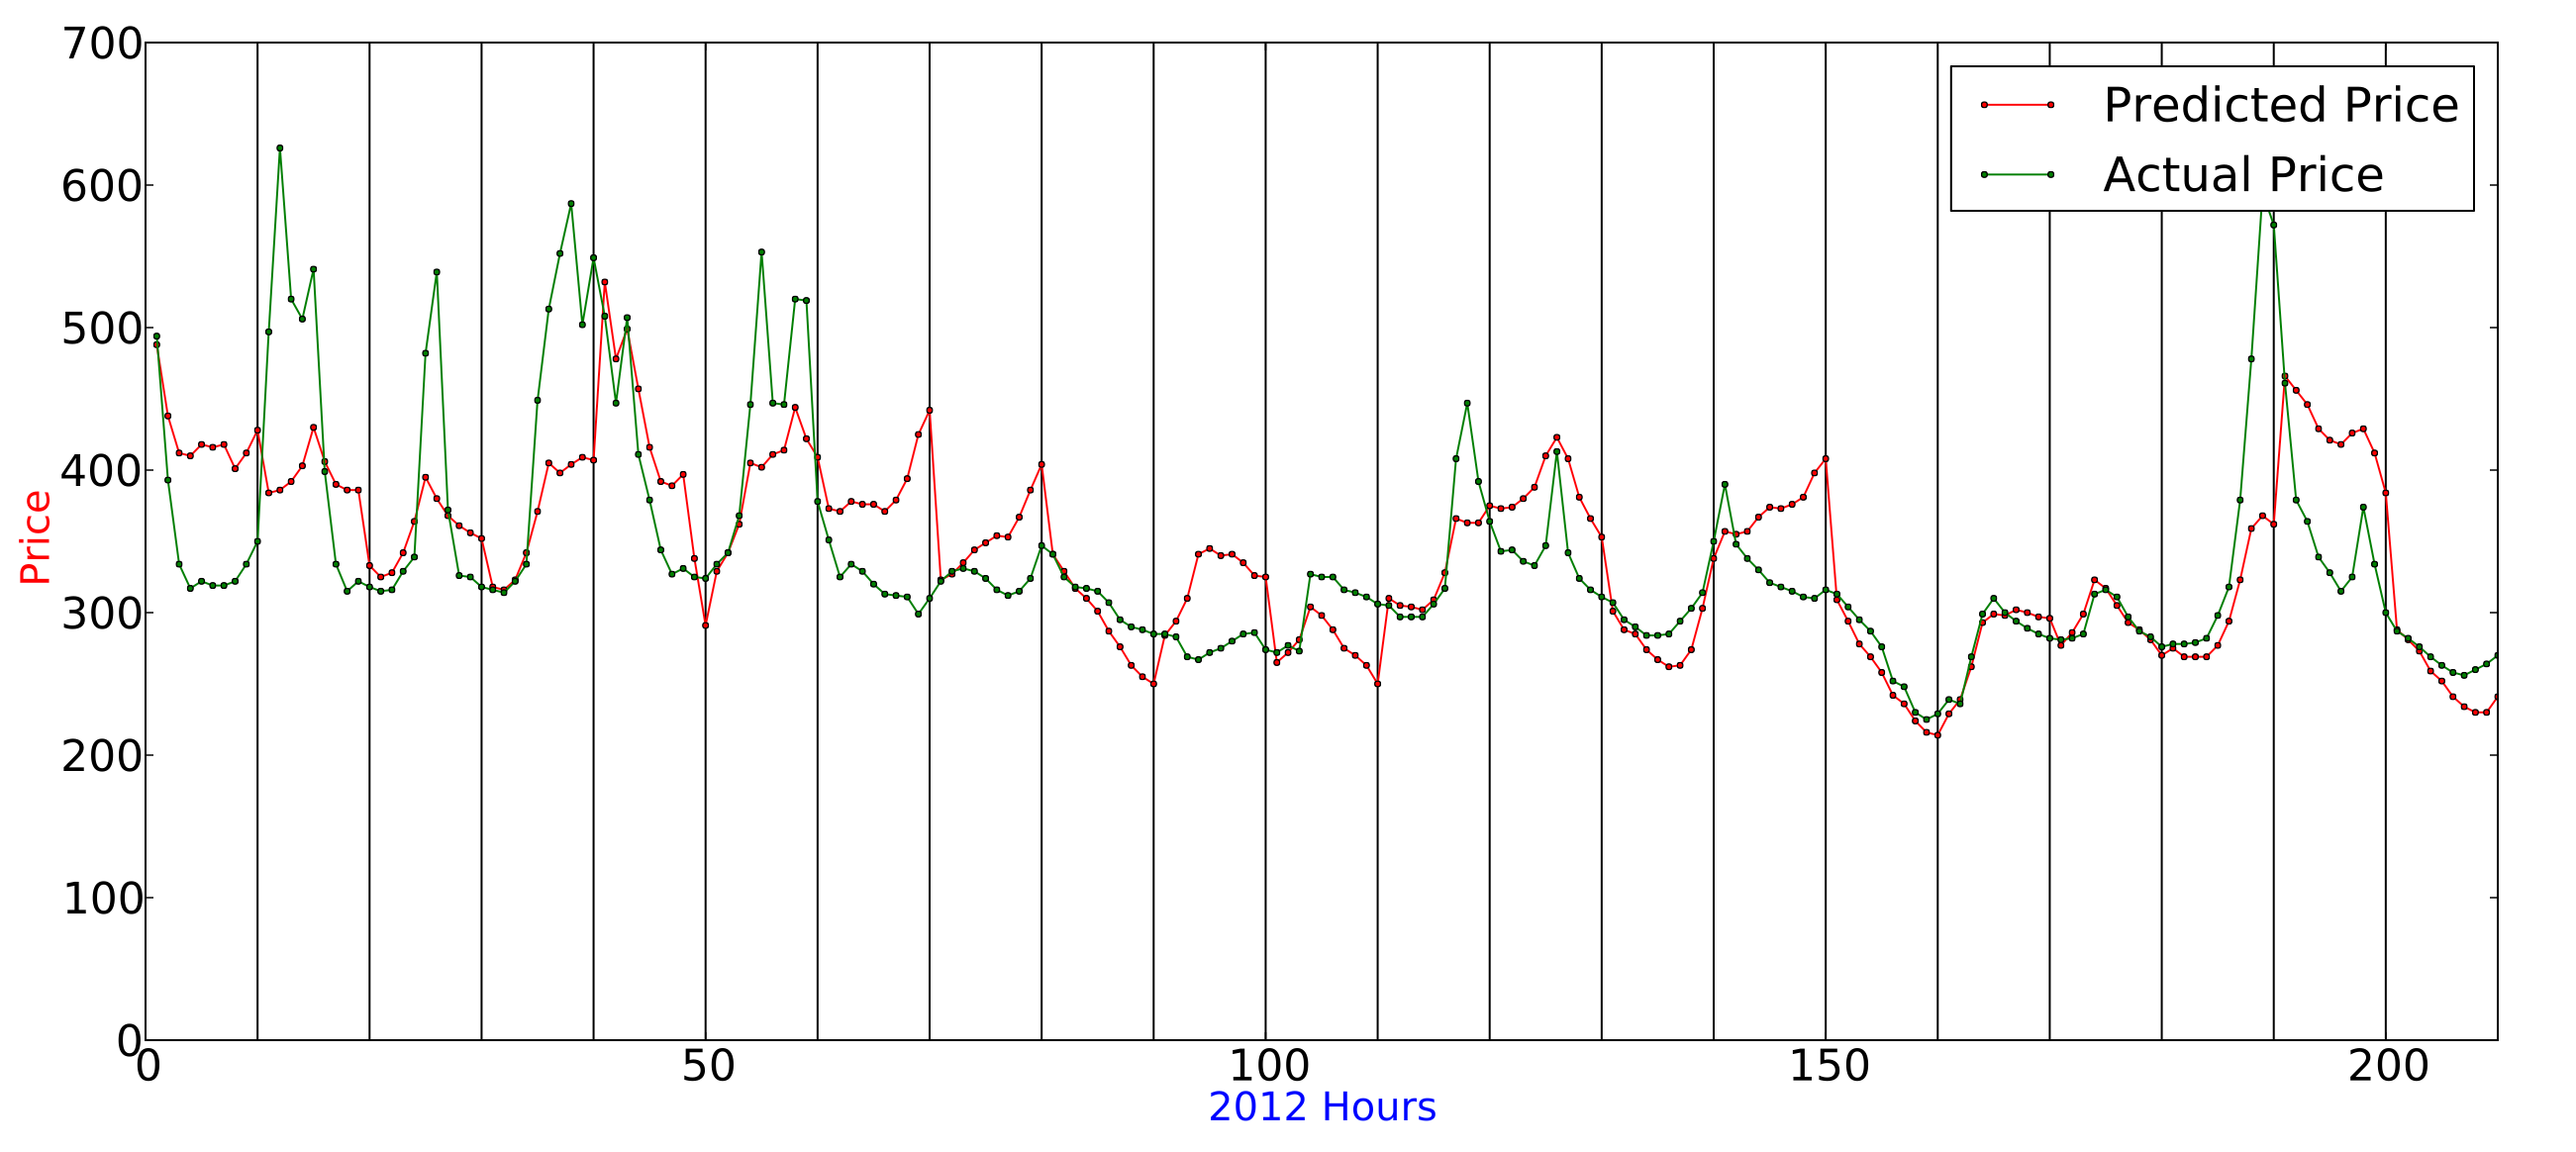
\includegraphics[width=\linewidth]{billeder/PriceExperimentalAnalysis/10HoursAhead.png}
\caption{Prediction of 10 hours ahead}
\label{fig:10HoursAhead}
\end{figure}

\begin{table}[H]
\centering  % used for centering table
\resizebox{0.8\textwidth}{!}{
	\begin{tabular}{|c|c|c|c|c|c|} % centered columns (7 columns)		
	\hline
	\# & Hours ahead & H1 & H2 & MAE & \% ranking\\ [0.5ex] % inserts table 
	\hline  
	1  & 1  & 5 & 1 & 22,17 & - \\ \hline
	2  & 2  & 5 & 1 & 28,29 & 27,64\% \\ \hline
	3  & 3  & 5 & 1 & 31,85 & 43,69\% \\ \hline
	4  & 4  & 5 & 1 & 34,68 & 56,44\% \\ \hline
	5  & 5  & 5 & 1 & 37,54 & 69,33\% \\ \hline
	6  & 6  & 5 & 1 & 39,69 & 79,08\% \\ \hline
	7  & 7  & 5 & 1 & 40,53 & 82,82\% \\ \hline
	8  & 8  & 5 & 1 & 42,23 & 90,52\% \\ \hline
	9  & 9  & 5 & 1 & 43,45 & 96,01\% \\ \hline
	10 & 10 & 5 & 1 & 44,10 & 98,94\% \\ \hline
	11 & 14 & 5 & 1 & 45,48 & 105,16\% \\ \hline
	12 & 11 & 5 & 1 & 45,73 & 106,3\% \\ \hline
	13 & 13 & 5 & 1 & 46,19 & 108,36\% \\ \hline
	14 & 12 & 5 & 1 & 46,67 & 110,52\% \\ \hline
	15 & 16 & 5 & 1 & 47,76 & 115,45\% \\ \hline
	16 & 15 & 5 & 1 & 48,05 & 116,75\% \\ \hline
	17 & 21 & 5 & 1 & 48,21 & 117,47\% \\ \hline
	18 & 19 & 5 & 1 & 48,69 & 119,64\% \\ \hline
	19 & 17 & 5 & 1 & 48,69 & 119,65\% \\ \hline
	20 & 18 & 5 & 1 & 49,00 & 121,04\% \\ \hline
	21 & 20 & 5 & 1 & 49,31 & 122,44\% \\ \hline
	22 & 22 & 5 & 1 & 49,75 & 124,45\% \\ \hline
	23 & 23 & 5 & 1 & 50,01 & 125,63\% \\ \hline
	24 & 24 & 5 & 1 & 50,87 & 129,48\% \\ \hline
	\end{tabular}
}
\caption{The results from the hours ahead predictions.} % title of Table
\label{table:XHoursAhead} % is used to refer this table in the text
\end{table}

In table~\ref{table:XHoursAhead} we see the results from the sliding window test. The entry with offset 0 is the same setup as prior experiments. The rest shows the difference in MAE when we shift where the 24 hours ahead predictions begin. We cover all possible offsets by doing 0-23 thus covering every offset from the first 24 hour prediction and onwards. From this experiment we show how much the right offset means for the total MAE in a years prediction. The biggest difference are between offset 4 and offset 7 with a difference of 15,04\%. These differences are connected to the elevation of error we talked about in the last result. If we hit the right spots where the elevation of error are not going to have a big impact this will lower the overall MAE thus giving us a better result.  

\begin{table}[H]
\centering  % used for centering table
\resizebox{0.8\textwidth}{!}{
	\begin{tabular}{|c|c|c|c|c|c|c|} % centered columns (7 columns)		
	\hline
	\# & Offset & Time(seconds) & H1 & H2 & MAE & \% ranking\\ [0.5ex] % inserts table 
	\hline 
	1  & 4  & 370,54 & 9  & 12 & 46,63 & - \\ \hline
	2  & 0  & 333,96 & 8  & 10 & 47,07 & 0,95\% \\ \hline
	3  & 8  & 364,68 & 8  & 12 & 47,29 & 1,41\% \\ \hline
	4  & 11 & 351,22 & 9  & 8  & 47,35 & 1,54\% \\ \hline
	5  & 14 & 358,79 & 8  & 11 & 47,45 & 1,75\% \\ \hline
	6  & 10 & 385,88 & 10 & 11 & 47,46 & 1,79\% \\ \hline
	7  & 21 & 339,93 & 8  & 9  & 47,58 & 2,04\% \\ \hline
	8  & 17 & 380,54 & 11 & 9  & 47,90 & 2,72\% \\ \hline
	9  & 1  & 345,99 & 7  & 15 & 48,11 & 3,18\% \\ \hline
	10 & 2  & 352,35 & 12 & 5  & 49,06 & 5,2\% \\ \hline
	11 & 12 & 406,33 & 13 & 11 & 49,09 & 5,28\% \\ \hline
	12 & 9  & 311,51 & 6  & 7  & 49,15 & 5,4\% \\ \hline
	13 & 13 & 410,08 & 13 & 11 & 49,84 & 6,87\% \\ \hline
	14 & 3  & 417,93 & 14 & 12 & 50,06 & 7,36\% \\ \hline
	15 & 19 & 404,45 & 11 & 12 & 50,87 & 9,1\% \\ \hline
	16 & 5  & 387,61 & 12 & 9  & 51,07 & 9,53\% \\ \hline
	17 & 20 & 404,6  & 7  & 24 & 51,41 & 10,25\% \\ \hline
	18 & 15 & 395,16 & 11 & 11 & 51,82 & 11,14\% \\ \hline
	19 & 16 & 409,38 & 13 & 10 & 51,91 & 11,32\% \\ \hline
	20 & 6  & 408,67 & 16 & 6  & 51,93 & 11,37\% \\ \hline
	21 & 22 & 448,74 & 17 & 9  & 52,00 & 11,52\% \\ \hline
	22 & 18 & 433,96 & 9  & 21 & 52,25 & 12,05\% \\ \hline
	23 & 23 & 349,56 & 8  & 10 & 53,02 & 13,7\% \\ \hline
	24 & 7  & 410,11 & 9  & 18 & 53,64 & 15,04\% \\ \hline
	\end{tabular}
}
\caption{The difference in MAE depending on the starting offset} % title of Table
\label{table:Offsets} % is used to refer this table in the text
\end{table}

\subsubsection{Conclusion}
In the hours ahead prediction we saw that the error margin was rising up until 10 hours ahead and from there only increasing slightly. This is because of the error margin not escalating infinitely but at some point will adapt to the changes in the other parameters pulling it in the right direction thus stopping the error from elevating further.

The offsets showed us a difference of 15,04\% from the best to the worst starting point. This difference in MAE is present because of how good a starting point the prediction will hit in general. The starting point is where the errors will start originating from; so if we can make the first prediction better the rest will in general also be better since we use the history of the curve to predict the next hourly price.

\newpage
\subsection{Concluding remarks}
We conducted a series of experiments where we tested the parameters we identified in the electricity price analysis section ~\ref{sec:ElectricityPriceAnalysis}. We have shown the results from 5 aspects of the price predicting artificial neural network we created. We presented how the different parameters and setups changes the output and accuracy of the ANN. In table~\ref{table:OverallImprovement} the best results from the experiments are presented and the overall improvement have been calculated to be 26.62\% from the initial tests to the best result in exp 3.

\begin{table}[H]
\centering  % used for centering table
\resizebox{0.8\textwidth}{!}{
	\begin{tabular}{|c|c|c|c|c|} % centered columns (7 columns)		
	\hline
	Exp 1 & Exp 2 & Exp 3 & Exp 4 & Overall improvement\\ [0.5ex] % inserts table 
	\hline 
	57.12 & 47,21 & 45,11 & 45.17 & 26.62\% \\ \hline
	\end{tabular}
}
\caption{The best results from the experiments and the overall improvement.} % title of Table
\label{table:OverallImprovement} % is used to refer this table in the text
\end{table}

\begin{enumerate}
	\item Experiment one: This experiment showed how the different input parameters influenced the accuracy of the ANN and how important it is to select the right inputs. We also experimented with the format of the inputs; which we either represented as a matrix or a single input node. The best combination from this test is what we based the rest of the tests on. The best test result gave us the combination of last known price, consumption, wind speed, temperature, the time of the day, the day of the week and the season of the year.
	\item Experiment two: We experimented with trimming and showed the benefits from trimming the dataset and the possible loss of accuracy on the upper and lower bound of the dataset. It only makes sense to trim the top and bottom of the dataset if extreme outliers are apparent in the dataset. We saw in the wind production experiment two~\ref{sec:windProdExperimentTwo} how trimming the dataset can have a negative effect on the outcome if the dataset does not contain extreme outliers. Trimming improved the price prediction by 20.99\% compared to the results from experiment one.
	\item Experiment three: This experiment shows the effect of adding calculated inputs to the ANN and how it improves the predictions. The calculated inputs improved the prediction of the results by 4.65\% and contained the EWMA and the skewness inputs. We also tested scattered prices where the ANN on its own makes the connections between the historical prices and the output these were only effective on the simplest of the datasets (price and consumption) but did not have any effect on the best combination from experiment one.
	\item Experiment four: Here we tested different black box optimizations such as number of epochs used to train the network and size of the dataset. The best result here gave us 45,17 which were 0.13\% worse than experiment three but this is probably because of the randomness factor that will always have and influence when working with predictions.
	\item Experiment five: Shows how the ANN is affected by changing the number of hours ahead it has to predict. The error margin increases quite a lot when we add more hours ahead to predict. This is because of the dependency on the last hours price; which for each hour predicted might add more error to the calculations. We also showed the influence of what offset we start the predictions from. This shows that a good starting position can improve the results by 15.04\% from the worst to the best starting offset.
\end{enumerate}

\todo{LAV TREND ANALYSE, LAV PRICE og CONSuMPTION graf}